%%%%%%%%%%%%%%%%%%%%%%%%%%%%%%%%%%%%%%%%%%%%%%%%%%%%%%%%%%%%%%%
%
%     filename  = "Dissertation Index.tex",
%     version   = "Draft 1",
%     date      = "1/16/2013",
%     authors   = "Nicholas P. Nicoletti",
%     copyright = "Nicholas P. Nicoletti",
%     address   = "Department of Political Science,
%                  516 Park Hall,
%                  University at Buffalo,
%                  Buffalo, NY 14260,
%                  USA",
%     telephone = "(585) 752-5167",
%     email     = "npn@buffalo.edu",
%
%%%%%%%%%%%%%%%%%%%%%%%%%%%%%%%%%%%%%%%%%%%%%%%%%%%%%%%%%%%%%%%
%
% Change History:
%
% Draft Version 1.0 - No Changes.
%
%%%%%%%%%%%%%%%%%%%%%%%%%%%%%%%%%%%%%%%%%%%%%%%%%%%%%%%%%%%%%%%
%
% This is a template file to help get you started using the
% psuthesis.cls for theses and dissertations at Penn State
% University. You will, of course, need to put the
% psuthesis.cls file someplace that LaTeX will find it.
%
% We have set up a directory structure that we find to be clean
% and convenient. You can readjust it to suit your tastes. In
% fact, the structure used by our students is even a little
% more involved and commands are defined to point to the
% various directories.
%
% This document has been set up to be typeset using pdflatex.
% About the only thing you will need to change if typesetting
% using latex is the \DeclareGraphicsExtensions command.
%
% The psuthesis document class uses the same options as the
% book class. In addition, it requires that you have the
% ifthen, calc, setspace, and tocloft packages.
%
% The first additional option specifies the degree type. You
% can choose from:
%     Ph.D. using class option <phd>
%     M.S. using class option <ms>
%     M.Eng. using class option <meng>
%     M.A. using class option <ma>
%     B.S. using class option <bs>
%     B.A. using class option <ba>
%     Honors Baccalaureate using the option <honors>
%
% If you specify either ba or bs in addition to honors, it will
% just use the honors option and ignore the ba or bs option.
%
% The second additional option <inlinechaptertoc> determines
% the formatting of the Chapter entries in the Table of
% Contents. The default sets them as two-line entries (try it).
% If you want them as one-line entries, issue the
% inlinechaptertoc option.
%
% The class option ``honors'' should be used for theses
% submitted to the Schreyer Honors College. This option
% changes the formatting on the Title page so that the
% signatures appear on the Title page. Be sure and comment
% out the command \psusigpage when using this option since it
% is not needed and it messes up the vertical spacing on the
% Title page.
%
% The class option ``honorsdepthead'' adds the signature of the
% department head on the Title page for those baccalaureate
% theses that require this.
%
% The class option ``secondthesissupervisor'' should be used
% for baccalaureate honors degrees if you have a second
% Thesis Supervisor.
%
% The vita is only included with the phd option and it is
% placed at the end of the thesis. The permissions page is only
% included with the ms, meng, and ma options.
%%%%%%%%%%%%%%%%%%%%%%%%%%%%%%%%%%%%%%%%%%%%%%%%%%%%%%%%%%%%%%%
% Only one of the following lines should be used at a time.
%\documentclass[draft,phd,12pt]{psuthesis}
\documentclass[draft,phd,12pt,inlinechaptertoc]{psuthesis}
%\documentclass[draft,ms]{psuthesis}
%\documentclass[draft,honorsdepthead,honors]{psuthesis}
%\documentclass[draft,honors]{psuthesis}
%\documentclass[draft,secondthesissupervisor,honors]{psuthesis}
%\documentclass[draft,bs]{psuthesis}
\renewcommand{\sfdefault}{ppl}
\renewcommand{\familydefault}{\sfdefault}

%%%%%%%%%%%%%%%%%%%%%%%%%%%%
% Packages we like to use. %
%%%%%%%%%%%%%%%%%%%%%%%%%%%%
\usepackage{amsmath}
\usepackage{amssymb}
\usepackage{amsthm}
\usepackage{exscale}
\usepackage[mathscr]{eucal}
\usepackage{bm}
\usepackage{eqlist} % Makes for a nice list of symbols.
\usepackage[final]{graphicx}
\usepackage[dvipsnames]{color}
\DeclareGraphicsExtensions{.pdf, .jpg, .png}
%\usepackage{natbib}
%\usepackage{har2nat}
\usepackage{verbatim}
\usepackage{url}
\usepackage{cite}
\usepackage{longtable}
\usepackage{mathpazo}
\usepackage{pstricks}
\usepackage{sgamevar}
\usepackage{soul}
\usepackage{egameps}
%\def\citeapos#1{\citeauthor{#1}'s \citeyear{#1}}
\newenvironment{my_enumerate}
{\begin{enumerate}
  \setlength{\itemsep}{1pt}
  \setlength{\parskip}{0pt}
  \setlength{\parsep}{0pt}}{\end{enumerate}}
\newenvironment{my_itemize}
{\begin{itemize}
  \setlength{\itemsep}{1pt}
  \setlength{\parskip}{0pt}
  \setlength{\parsep}{0pt}}{\end{itemize}}
\usepackage{geometry}
\geometry{total={210mm,297mm},left=25mm,right=25mm,top=40mm,bottom=30mm}

%%%%%%%%%%%%%%%%%%%%%%%%
% Setting for fncychap %
%%%%%%%%%%%%%%%%%%%%%%%%
% Comment out or remove the next two lines and you will get
% the standard LaTeX chapter titles. We like these A LOT
% better.
\usepackage[Lenny]{fncychap}
\ChTitleVar{\Huge\sffamily\bfseries}

%%%%%%%%%%%%%%%%%%%%%%%%%%%%%%%
% Use of the hyperref package %
%%%%%%%%%%%%%%%%%%%%%%%%%%%%%%%
%
% This is optional and is included only for those students
% who want to use it.
%
% To use the hyperref package, uncomment the following line:
\usepackage[colorlinks]{hyperref}
%
% Note that you should also uncomment the following line:
\renewcommand{\theHchapter}{\thepart.\thechapter}
%
% to work around some problem hyperref has with the fact
% the psuthesis class has unnumbered pages after which page
% counters are reset.


%%%%%%%%%%%%%%%%%%%%%%%%%%%%%%%%%%%%
% SPECIAL SYMBOLS AND NEW COMMANDS %
%%%%%%%%%%%%%%%%%%%%%%%%%%%%%%%%%%%%
% Place user-defined commands below.
\newcommand{\abInitio}[0]{\emph{ab initio} }
\newcommand{\AbInitio}[0]{\emph{Ab initio} }
\newcommand{\Schrodinger}[0]{Schr\"{o}dinger }



%%%%%%%%%%%%%%%%%%%%%%%%%%%%%%%%%%%%%%%%%
% Renewed Float Parameters              %
% (Makes floats fit better on the page) %
%%%%%%%%%%%%%%%%%%%%%%%%%%%%%%%%%%%%%%%%%
\renewcommand{\floatpagefraction}{0.85}
\renewcommand{\topfraction}      {0.85}
\renewcommand{\bottomfraction}   {0.85}
\renewcommand{\textfraction}     {0.15}

% ----------------------------------------------------------- %

%%%%%%%%%%%%%%%%
% FRONT-MATTER %
%%%%%%%%%%%%%%%%
% Title
\title{QUANTUM VIRIAL COEFFICIENTS VIA PATH INTEGRAL MONTE CARLO: THEORY AND DEVELOPMENT OF NOVEL ALGORITHMS}

% Author and Date of Degree Conferral or Defense
\author{Ramachandran Subramanian}
% the degree will be conferred on this date
\degreedate{May 9, 2016}
% year of your copyright. I have removed this from the cover page because UB's guidelines do not include it.
\copyrightyear{2016}

% This is the document type. For example, this could also be:
%     Comprehensive Document
%     Thesis Proposal
\documenttype{Disseration}
%The department where you will be submitting the document%
\dept{Department of Chemical and Biological Engineering}
% This will generally be The Graduate School, though you can
% put anything in here to suit your needs. This has also been removes from the cover page via the psuthesis.cls document because UB guidelines do not allow for it.
\submittedto{The Graduate School}


%%%%%%%%%%%%%%%%%%
% Signatory Page %
%%%%%%%%%%%%%%%%%%
% You can have up to 7 committee members, i.e., one advisor
% and up to 6 readers.
%
% Begin by specifying the number of readers.
\numberofreaders{3}


% Input reader information below. The optional argument, which
% comes first, goes on the second line before the name.
\advisor[Thesis Advisor, Chair of Committee]
        {David A. Kofke}
        {SUNY Distinguished Professor}

\readerone[Committee Member]
          {Andrew J. Schultz}
          {Research Assistant Professor}

\readertwo[Committee Member, Associate Dean for Undergraduate Education]
          {Jeffrey R. Errington}
          {Professor}

\readerthree[Committee Member]
            {Johannes Hachmann}
            {Assistant Professor}

\readerfour[Optional Title Here]
           {Reader Name}
           {Professor of SomeThing}

\readerfive[Optional Title Here]
           {Reader Name}
           {Professor of SomeThing}

% Makes use of LaTeX's include facility. Add as many chapters
% and appendices as you like.
\includeonly{%
Chapter-1/Chapter-1,%
Chapter-2/Chapter-2,%
Chapter-3/Chapter-3,%
Chapter-4/Chapter-4,%
Chapter-5/Chapter-5,%
Chapter-6/Chapter-6,%
Chapter-7/Chapter-7,%
Chapter-8/Chapter-8,%
Chapter-9/Chapter-9,%
Chapter-10/Chapter-10,%
Appendix-A/Appendix-A,%
Appendix-B/Appendix-B%
}

%%%%%%%%%%%%%%%%%
% THE BEGINNING %
%%%%%%%%%%%%%%%%%
\begin{document}
%%%%%%%%%%%%%%%%%%%%%%%%
% Preliminary Material %
%%%%%%%%%%%%%%%%%%%%%%%%
% This command is needed to properly set up the frontmatter.
\frontmatter

%%%%%%%%%%%%%%%%%%%%%%%%%%%%%%%%%%%%%%%%%%%%%%%%%%%%%%%%%%%%%%
% IMPORTANT
%
% The following commands allow you to include all the
% frontmatter in your thesis. If you don't need one or more of
% these items, you can comment it out. Most of these items are
% actually required by the Grad School -- see the Thesis Guide
% for details regarding what is and what is not required for
% your particular degree.
%%%%%%%%%%%%%%%%%%%%%%%%%%%%%%%%%%%%%%%%%%%%%%%%%%%%%%%%%%%%%%
% !!! DO NOT CHANGE THE SEQUENCE OF THESE ITEMS !!!
%%%%%%%%%%%%%%%%%%%%%%%%%%%%%%%%%%%%%%%%%%%%%%%%%%%%%%%%%%%%%%

% Generates the signature page. This is not bound with your
% thesis.
%\psusigpage

% Generates the title page based on info you have provided
% above.
\psutitlepage

%Generates Copyright Page
\copyrightpage{SupplementaryMaterial/Copyright}

\newpage
% Generates the committee page -- this is bound with your
% thesis. If this is an baccalaureate honors thesis, then
% comment out this line.
%\psucommitteepage

% Generates the Epigraph/Dedication. The first argument should
% point to the file containing your Epigraph/Dedication and
% the second argument should be the title of this page.
\thesisdedication{SupplementaryMaterial/Dedication}{Dedication}

% Generates the Acknowledgments. The argument should point to
% the file containing your Acknowledgments.
\thesisacknowledgments{SupplementaryMaterial/Acknowledgments}

% Generates the Table of Contents
\thesistableofcontents

% Generates the List of Tables
\thesislistoftables

% Generates the List of Figures
\thesislistoffigures

% Generates the List of Symbols. The argument should point to
% the file containing your List of Symbols.
%\thesislistofsymbols{SupplementaryMaterial/ListOfSymbols}

% Generates the abstract. The argument should point to the
% file containing your abstract.
\thesisabstract{SupplementaryMaterial/Abstract}


%%%%%%%%%%%%%%%%%%%%%%%%%%%%%%%%%%%%%%%%%%%%%%%%%%%%%%
% This command is needed to get the main part of the %
% document going.                                    %
%%%%%%%%%%%%%%%%%%%%%%%%%%%%%%%%%%%%%%%%%%%%%%%%%%%%%%
\thesismainmatter

%%%%%%%%%%%%%%%%%%%%%%%%%%%%%%%%%%%%%%%%%%%%%%%%%%
% This is an AMS-LaTeX command to allow breaking %
% of displayed equations across pages. Note the  %
% closing the "}" just before the bibliography.  %
%%%%%%%%%%%%%%%%%%%%%%%%%%%%%%%%%%%%%%%%%%%%%%%%%%
\allowdisplaybreaks{
%
%%%%%%%%%%%%%%%%%%%%%%
% THE ACTUAL CONTENT %
%%%%%%%%%%%%%%%%%%%%%%
% Chapters
\chapter{Background and Motivation} \label{chap:background and motivation}
    \section{Virial coefficients}
        The virial equation of state, given as:
        \begin{equation}
          \frac{p}{\rho k_\textrm{B}T} = 1 + B_2(T) \rho + B_3(T) \rho^2 + \ldots,
        \end{equation}
        expresses the pressure $p$ as a power series in the number density $\rho$ of the system; $T$ is the temperature and $k_\textrm{B}$ is the Boltzmann constant. Through this formula, the temperature-dependent virial coefficients, $B_n(T)$, can be used to estimate a variety of physical properties in addition to the pressure, such as the Joule-Thomson coefficient,  critical properties, and others. The unique feature of the virial equation of state, in comparison to other thermodynamic models, is that it represents rigorously the effect of interactions among $N$ molecules, such that if given a molecular model, the virial coefficients for its equation of state can be determined without approximation. This can be clearly seen from the analytic expressions for the virial coefficients in terms of $N$-body configurational integrals \cite{Tester} which depend only on the interaction potential between $N$ molecules as:
        \begin{equation}\label{eq: bn}
            \begin{aligned}
                B_2(T) &= - \frac{1}{2! {V}}  \Big[ Z_2^* - Z_1^{*2} \Big]\\
                B_3(T) &= - \frac{1}{3! {V}^2}  \Big[ {V}  \big( Z_3^* - 3  Z_2^*  Z_1^* + 2  Z_1^{*3} \big) - 3  {\big( Z_2^* - Z_1^{*2} \big)}^2 \Big]
            \end{aligned}
        \end{equation}
        where, $ Z_N^* \equiv N!  {\Big( \displaystyle\frac{{V}}{Q_1} \Big)}^N  Q_N ;$ is the $N$-body configurational integral, $Q_N$ is the $N$-body canonical partition function, and ${V}$ is the volume.

        The $N$-body configurational integral, which depends on the $N$-body interaction potential, becomes exponentially more difficult to compute with increasing $N$ (\hl{include the exact numbers from Hansen}). For extremely simple interaction potentials like hard spheres, up to fourth virial coefficients may be calculated analytically \cite{Masters2008}. Higher order virial coefficients using more complicated interaction potentials need to be evaluated numerically through quadrature or by using Monte Carlo (MC) simulations. Upon further simplification and assuming pairwise additivity (\hl{may be include more detailed formulae}) of the potential, we can rewrite Eq.\eqref{eq: bn} using Mayer $f$-functions as \cite{Masters2008,Hansen}
        \begin{equation} \label{eq: mayerfn}
            \begin{aligned}
                B_2(T) &= -\frac{1}{2} \displaystyle\int d1 ~ f(0,1)\\
                B_3(T) &= -\frac{1}{3} \displaystyle\int \int d1~d2~f(0,1)~f(0,2)~f(1,2)
            \end{aligned}
        \end{equation}
        where $f(0,1) = \Big( \exp \big[ -\beta U_2(\bm{r}) \big] - 1 \Big) $ and indices `1' and `2' denote the position and orientational degrees of freedom of molecules 1 and 2, respectively, with respect to molecule `0' at the origin.

        Virial coefficients can be evaluated in two ways: a) computationally, using numerical methods to evaluate the configuration integrals given an input interaction potential, and b) experimentally, typically by collecting pressure-density data and regressing its behavior at the $\rho \to 0$ limit. By comparing the values determined using the above two methods, different models of the interaction potential between $N$ molecules can be ranked for their physical accuracy.

        Empirical potentials are fit to experimental data over a broad range of conditions, and therefore they tend to describe the interaction potential as the net result of a variety of physical phenomena taking place simultaneously (including, for example, multibody interactions and nuclear quantum effects). The way that these phenomena combine to give an effective potential will depend on the state condition as well as the experimental properties being fit. Consequently, unless fit directly to them, empirical potentials often perform poorly in comparison to experimental virial coefficients \cite{Benjamin2007}, which depend purely on the interaction of a specific number of molecules.

        On the other hand, \abInitio{} potentials involve solving the \Schrodinger{} equation by using different basis functions and levels of theory and often can yield far more accurate interaction potentials as a result. Large computational resources are required to obtain coefficient with a useful level of accuracy, so the application of \abInitio{} method in this respect has been limited to low-order coefficients for small molecules. However, steady progress is being made \cite{Boothroyd2003,Hodges2004,Garberoglio2012,Shaul2012,Garberoglio2013,Hellmann2013,Garberoglio2014,Garberoglio2014mix,Hellmann2014,Schultz2015,Tat2015}. Almost all \abInitio{} potentials involve at the heart of their development, solving the electronic \Schrodinger{} equation using the Born-Oppenheimer approximation. Under this approximation, the kinetic energy of the nucleus is considered negligible when compared to the electrons, and therefore all the nuclei are assumed to be fixed at certain locations when solving the electronic structure. For the purpose of calculating really virial accurate coefficients using \abInitio{} potentials, one needs to account for nuclear quantum effects explicitly, especially at low temperatures or for light atoms, such as hydrogen. Based on the above, virial coefficients can be classified into the following three categories:

        \begin{description}
            \item[Classical virial coefficients] \hfill \\
                The virial coefficients that are calculated from an input interaction potential (empirical or \abInitio{} PES) without modification.
            \item[Semi-classical virial coefficients] \hfill \\
                The virial coefficients that are calculated using an effective potential such as the Quadratic Feynman-Hibbs (QFH) \cite{Feynman} that includes a quantum correction.
            \item[Quantum virial coefficients] \hfill \\
                The virial coefficients that are calculated using an empirical potential (quantum) or \abInitio{} PES (fully quantum) while explicitly including nuclear quantum effects.
        \end{description}
    \section{\AbInitio{} Potentials}
        In this section, different quantum chemistry methods and theories that are used in the development of the \abInitio{} \PESs{} are briefly mentioned. This will help develop an idea of the amount of computational effort involved in such calculations, which will later be called upon to serve as motivation for developing efficient algorithms in Chapter \ref{sec:novel algorithms}. Majority of what follows in this section is directly adapted from Chapter's 4, 6 and 7 of Cramer's book \cite{Cramer} (where the interested reader may also find more comprehensive and mathematically detailed explanations) and are only intended as a precursor to better understanding the rest of this dissertation work. \\
        \subsection{From \Schrodinger{} equation to Molecular Orbitals}
            We begin by considering the \Schrodinger{} equation and the Hamiltonian operator, $H$ of a generic atom:
            \begin{equation}\label{eq:Schrodinger}
                \begin{aligned}
                    H~\Psi &= E~\Psi \\
                    H &= T_e + T_N + V_{ee} + V_{eN} + V_{NN}
                    %\ham{H}      &= -\displaystyle\sum_i \frac{\hbar^2}{2 m_e} \nabla^2_i -\displaystyle\sum_k \frac{\hbar^2}{2 m_k} \nabla^2_k + \displaystyle\sum_i \displaystyle\sum_k \frac{e^2 Z_k}{r_{ik}} + \displaystyle\sum_{i<j} \frac{e^2}{r_{ij}} +\displaystyle\sum_{k<l} \frac{e^2 Z_k Z_l}{r_{kl}}
                \end{aligned}
            \end{equation}
            where $T$ and $V$ represent the kinetic and potential energy operators respectively; the subscripts $e$ and $N$ denote the elctron and the nucleus respectively.

            The eigenfunctions of Eq. \eqref{eq:Schrodinger} are known as the wavefunctions of the atom and are denoted as $\Psi_i$. For ease of explanation, we only consider wavefunctions that are orthonormal, i.e., they satisfy the following the condition:
            \begin{equation}\label{eq:orthonormality}
                \int \Psi_i\, \Psi_j\, d\, \mathbf{r} = \delta_{ij}
            \end{equation}
            where $\delta_{ij}$ is the Kronecker delta.

            Given a complete set of orthonormal wavefunctions, it is then possible to compute the expectation value of any physical property $A$, by expressing it in operator form $\hat{A}$, and evaluating:
            \begin{equation}\label{eq:expectation value}
                <\,A\,>\, =\, < \,\Psi_i\,|\,\hat{A}\,|\, \Psi_j\,>
            \end{equation}
            Knowing the wavefunction of a system exactly is therefore equivalent to possessing all information required about the system. Since there will always exist a ground state configuration of a system, the variational principle allows us to rank different sets of wavefunctions based on their energies w.r.t the ground state energy. According to the variational principle, the lower the energies, the better the set of wavefunctions. Therefore one can, in principle, devise a mechanism to construct and gradually improve the set of wavefunctions to find the best possible set of wavefunctions using various mathematical tools.

            The \Schrodinger{} equation is inherently complicated due to the correlation of interactions of many particles with one another, as expressed in Eq. \eqref{eq:Schrodinger}. However, there are certain approximations and assumptions that reduce the complexity of the equation. For instance, the Born-Oppenheimer(BO) approximation assumes that under ambient conditions, the motion of the nuclei are much slower compared to that of the electrons, owing to heavier masses. This makes it possible to separate the electronic and nuclear motions within the Hamiltionian $H$ (Eq. \eqref{eq:Schrodinger}) by setting $T_N \to 0$ and $V_N$ to some constant value. Whereas previously $H$ was dependent on the nuclear coordinates and electronic coordinates explicitly, using the BO approximation $H_{BO}$ depends explicitly only on electronic coordinates and the nuclear coordinates become parameters:
            \begin{equation}\label{eq:BO approximation}
                \begin{aligned}
                    (H_{BO} + V_N)~\Psi_{el} (\mathbf{q}_i;\mathbf{q}_k) &= E_{BO} \Psi_{el} (\mathbf{q}_i;\mathbf{q}_k)\\
                    H_{BO} &= T_e + V_{eN} + V_{ee}
                \end{aligned}
            \end{equation}

            Both the variational principle and the BO approximation have profound implications in quantum chemistry. Without the variational principle, it would not be possible to check and improve the mechanism of construction of orthonormal sets of wavefunctions. The PES, defined as $E_{BO}$ for different nuclear configurations ($\mathbf{q}_k$), would not exist if it were not for the BO approximation. Although the BO approximation significantly simplifies the \Schrodinger{} equation, the complexity due to the number of particles is still a challenge.

            The concept of constructing the set of orthonormal wavefunctions for many particle systems needs a starting point. Using the BO approximation for a system like the hydrogen atom with just one electron and one nucleus, analytical solutions can be obtained for the orthonormal set of wavefunctions or Atomic Orbitals(AOs). These then, become the perfect starting point for more complicated wavefunctions (called Molecular Orbitals(MOs)) by using what is known as the Linear Combination of Atomic Orbitals(LCAO) basis set approach. Within this approach, we use AOs as basis sets and construct linear combinations of them with different weights to give rise to MO wavefunction for many electron systems. Naturally, the more the number of basis functions in the basis set, the better the description of the resulting MO.

            Starting with $N$ wavefunctions $\{\psi_1, \psi_2, \ldots \psi_N\}$ as our basis set, we seek coefficients $a_{i}$ which will yield the minimum energy for the resulting MO wavefunction $\Psi = \displaystyle\sum_{i=1}^N a_{i} \psi_i$. The following is the procedure to obtain the MO wavefunction :
            \begin{enumerate}
                \item Determine all $N^2$ values of $H_{ij}$ and $S_{ij}$ which are also known as the 'resonance integral' and 'overlap integral' respectively.
                    \begin{equation}\label{eq:resonance and overlap}
                        \begin{aligned}
                            H_{ij} &= \displaystyle\int \psi_i\, H \,\psi_j\, d\,\mathbf{r}\\
                            S_{ij} &= \displaystyle\int \psi_i\, \psi_j\, d\,\mathbf{r}
                        \end{aligned}
                    \end{equation}
                    It should be noted that in practice, one would compute the values the matrix elements $H_{ij}$ from experimental data such as the ionization energy and rotational barriers. Also, we have assumed that the MO does not depend on the number of electrons present in the AO that form part of the basis set. Therefore, one might be tempted to say that the LCAO approach ignores the electron-electron repulsion. However, since we are deriving the matrix elements from experimental measurements, one might think of it as implicitly including the inter-electronic repulsion, albeit in a crude sense.
                \item Determine the $N$ roots $E_j$ of the secular equation given by:
                    \begin{equation}\label{eq:secular}
                        \begin{vmatrix}
                            H_{11} - E S_{11} & H_{12} - E S_{12} & \ldots & H_{1N} - E S_{1N}\\
                            H_{21} - E S_{21} & H_{22} - E S_{22} & \ldots & H_{2N} - E S_{2N}\\
                            \vdots & \vdots & \ddots & \vdots\\
                            H_{N1} - E S_{N1} & H_{N2} - E S_{N2} & \ldots & H_{NN} - E S_{NN}
                        \end{vmatrix}
                        = 0
                    \end{equation}
                \item For each of the $N$ values of $E_j$, solve the set of linear equations:
                    \begin{equation}\label{eq:linear}
                        \displaystyle\sum_{i=1}^N a_i (H_{ki} - E S_{ki}) = 0 \:\:\:\:\: \forall k
                    \end{equation}
            \end{enumerate}

            Upon careful observation Hartree noticed that if we set the term $V_{ee} \to 0$, the Hamiltonian in Eq. \eqref{eq:BO approximation} is separable into one-electron Hamiltonians which satisfy the one-electron \Schrodinger{} equation as defined below:
            \begin{equation}\label{eq:one electron H}
                \begin{aligned}
                    H &= \displaystyle\sum_i^N h_i\\
                    h_i &= -\frac{1}{2} \nabla^2_i - \frac{Z_k}{r_{ik}}\\
                    h_i\,\psi_i\, &= \epsilon_i \, \psi_i
                \end{aligned}
            \end{equation}
            where $\psi_i$ are the corresponding one-electron wavefunctions.

            Hartree then defined the many electron wavefunction as a product of these $\allowbreak$ one-electron wavefunctions. To account for the fact that one-electron Hamiltonians completely ignored the inter-electronic repulsion, Hartree approximated the net repulsion as an average potential and defined the correct Hamiltonian as shown below:
            \begin{equation}\label{eq:correct Hamiltonian}
                \begin{aligned}
                    h_i &= -\frac{1}{2} \nabla^2_i - \frac{Z_k}{r_{ik}} + V_i \{j\}\\
                    V_i \{j\} &= \displaystyle\sum_{j \ne i} \int \frac{\rho_j}{r_{ij}} d\,\mathbf{r}
                \end{aligned}
            \end{equation}
            where $V_i \{j\}$ represents the interaction potential with all the other electrons occupying orbitals $\{j\}$ and $\rho_j = |\psi_j|^2$; is the charge density associated with electron $j$.

            From Eq. \eqref{eq:correct Hamiltonian} it can be easily seen that $\psi_j$ is needed as input to obtain the correct Hamiltonian which would ultimately result in the correct wavefunction. Therefore this posed a problem of computing a quantity that required itself as an input. Hartree proposed an iterative Self Consistent Field(SCF) method as a solution to this problem. At the first step of this method, we guess the values of all $\psi_j$ and use them to construct the correct Hamiltonian operators as per Eq. \eqref{eq:correct Hamiltonian}. Using these operators, the one-electron \Schrodinger{} equation (Eq. \eqref{eq:one electron H}) is solved multiple times to obtain a new guess for all $\psi_j$. The process is then repeated until the results have converged based on some threshold value for the electronic energy.

            Since Hartree's product wavefunctions violated the property of indistinguishability of quantum particles and also ignored quantum mechanical exchange, a correlation effect unique to electrons of the same spin, Slater determinants provided an alternative route to incorporate these effects in the wavefunctions. By construction, Slater determinants accounted for the anti-symmetry and electronic spin (and hence exchange) which was crucial to MO wavefunctions. Expressed in determinant form as:
            \begin{equation}\label{eq:Slater determinant}
                \Psi_{SD} = \frac{1}{\sqrt{N!}}
                \begin{vmatrix}
                    \chi_1 (1) & \chi_2 (1) & \ldots & \chi_N (1)\\
                    \chi_1 (2) & \chi_2 (2) & \ldots & \chi_N (2)\\
                    \vdots & \vdots & \ddots & \vdots\\
                    \chi_1 (N) & \chi_2 (N) & \ldots & \chi_N (N)\\
                \end{vmatrix}
            \end{equation}
            where $N$ is the total number of electrons and $\chi$ is a spin-orbital, i.e., a product of the spatial oribital and an electron spin eigenfunction.

            Fock first proposed to extend the Hartree SCF method for Slater determinant wavefunctions giving rise to Slater Type Orbitals (STOs) and the Hartree-Fock(HF) SCF method$\allowbreak$, to which Roothaan \cite{Roothaan1951} made valuable contributions later. The 'restricted Hartree-Fock' (RHF) formalism with closed-shell systems and wavefunctions represented as a single Slater determinant is the typical form of the HF SCF method. The procedure to be followed using this approach is outlined below:
            \begin{enumerate}
                \item Choose a basis set and a molecular geometry
                \item Guess the intial density matrix $\mathbf{P}^{(0)}$ whose elements are given as:
                    \begin{equation}\label{eq:density matrix elements}
                        P_{\lambda \sigma} = 2 \displaystyle\sum_i^{occupied MO} a_{\lambda i} a_{\sigma i}
                    \end{equation}
                    where the coefficients $a_{\zeta i}$ specify the contribution of basis function $\zeta$ to the MO $i$ and the factor of two appears because with RHF theory we are considering only singlet wavefunctions in which all orbitals are doubly occupied.
                \item Construct and solve the HF secular equation which uses the Fock operator matrix elements in place of the Hamiltonian operator matrix elements in Eq. \eqref{eq:secular} as:
                    \begin{equation}\label{eq:one electron Fock matrix elements}
                        \begin{aligned}
                            f_i &= -\frac{1}{2} \nabla^2_i - \displaystyle\sum_k^{nuclei} \frac{Z_k}{r_{ik}} + V_i^{HF} \{j\}\\
                            F_{\mu \nu} &= \left< \mu \,\left| -\frac{1}{2} \nabla^2 \right|\,\nu \right> - \displaystyle\sum_k^{nuclei} Z_k \left< \mu \,\left| \frac{1}{r_k} \right| \, \nu \right> + \displaystyle\sum_{\lambda \sigma} P_{\lambda \sigma} \left[ (\mu \nu | \lambda \sigma) - \frac{1}{2} (\mu \lambda | \nu \sigma) \right]\\
                            (\mu \nu | \lambda \sigma) &= \displaystyle\int \int \phi_\mu (1) \phi_\nu(1) \frac{1}{r_{12}}\phi_\lambda (2) \phi_\sigma (2) d\,\mathbf{r}(1)\,d\,\mathbf{r}(2)
                        \end{aligned}                    
                    \end{equation}
                    where $\phi_\mu$ and $\phi_\nu$ represent the probability density of one electron and $\phi_\lambda$ and $\phi_\sigma$ the other. The exchange integrals $(\mu \nu | \lambda \sigma)$ are also known as the 'four index integrals' and are preceeded by a factor of 1/2 because they are limited to electrons of the same spin while Coulomb interactions are present in any combination of spins.
                \item Obtain new density matrix $\mathbf{P}^{(1)}$.
                \item Repeat steps 3. and 4. until convergence.
            \end{enumerate}
            
        \subsection{Basis Sets and Molecular Orbital Theory}
       
            HF SCF theory approximated the electron correlation effects as an average repulsive potential that each electron experiences and involved the use of different basis sets. The HF limit is defined as the case when the number of basis functions used in the basis set $\to \infty$. The amount of computational resources required for a practical calculation at the HF limit is extremely large. Therefore the choice of the basis set becomes important and there are three main guidelines to follow:
            \begin{enumerate}
               \item Computational complexity increases with increase in the number of basis functions and so, ideally this number should be as low as possible.
               \item The type of functions used should be in such a way that they facilitate easy evaluation of the four index integrals (Eq. \eqref{eq:one electron Fock matrix elements}). Hence, a large number of easily integrable basis functions might be preferred over a small number of difficult-to-integrate basis functions.
               \item The shape of the functions chosen should make some chemical sense, i.e., the amplitude of the function should be high in places where the probability density of finding the electron would be high and vice-versa.
            \end{enumerate}


            Considering the above mentioned factors, the STOs are rather unfavorable because they lead to four index integrals that are not easily integrable. To overcome this computational problem, Gaussian Type Orbitals(GTOs) were introduced that comprised of a quicker radial decay component than their STO counterparts. Although computationally convenient, because of the alterations to the shape brought about by using a different radial decay function, GTOs were seldom used directly as the basis functions in calculations. Also, since GTOs don't exhibit radial nodal behavior, using them one would not be able to mimic, for instance, the 2s orbital which should be negative near the origin and positive beyond a certain distance. To solve these problems, a linear combination of the GTOs were used to obtain basis functions that resembled the STOs as closely as possible. Such basis sets were known as 'contracted' basis sets and the original Gaussians used were known as the 'primitive' Gaussians. For instance:
            \begin{equation}\label{eq:contracted}
               \varphi(x, y, z; {\alpha}, i, j, k) = \displaystyle\sum_{a = 1}^M c_a \phi(x, y, z; \alpha_a, i , j, k)
            \end{equation}
            where $M$ is the number of Gaussians used in the linear combination, and the coefficients $c$ are chosen to optimize the shape of the basis function sum and ensure normalization.
            
            After performing various calculations, Hehre et al. \cite{Hehre1969} observed that using $M = 3$ primitive Gaussians was the optimum choice in terms of speed and accuracy when comparing to calculations using STOs. Since this is very small as compared to the HF limit, one way to add more flexibility to the basis set would be 'decontract' the basis functions. In other words, keeping the basis set same, we now construct more basis functions for each AO which would result in an increase in size of the secular equation (Eq. \eqref{eq:secular}). Accordingly, using only one basis function per AO is known as 'single-$\zeta$' basis, using two basis functions per AO is known as 'double-$\zeta$' basis and so on. The advantage of this scheme is that using larger and larger basis sets leads us to the HF limit. Since core orbitals tend to be less affected than the valence orbitals during chemical bonding, the 'decontracting' scheme is done more to the valence orbitals than to the core giving rise to 'split-valence' or 'valence-multiple-$\zeta$' basis sets.

            All basis sets considered until now, have been comprised of functions that are centered on the atoms. The use of such atom centered AOs to describe a molecule with multiple nuclei located at different positions could lead to erroneous results calculated even at near HF limit (for instance, HF calculations predict that a planar structure for NH$_3$ has the lowest energy). To avoid this behavior and to allow more flexibility to the MOs, polarization functions were introduced in the basis sets. It was also observed that there is a rough equality between each decontraction step for the valence electrons and adding one new set of polarization functions, including a new set of higher angular momentum.

            In addition to using polarization functions, diffuse functions are also used leading to what are known as 'augmented' basis sets. This is done so as to let the highest energy MOs, weakly bonded atoms and similar cases be more flexible. In practice, the names of basis sets contains information on what kinds of functions were used in their construction. For instance, the 'aug-cc-pVnZ' (read as 'augmented-coupled cluster- polarizable Valence n-$\zeta$') basis set uses diffuse functions on all atoms, uses coupled cluster theory (see Sec. \ref{sec:electron correlation} for more details) for electron correlation, uses polarizable functions with valence-multiple-$\zeta$ basis with Single(n = 1)-/Double(n = 2)-/Triple(n = 3)-/Qudaruple(n = 4)-/5-/6-$\zeta$ basis functions per AO. As it accounts for a variety of phenomena, one can confidently say that using such a basis set with increasing n would lead to the most accurate value at the HF limit for any desired property. To compute this value, one would simply evaluate the desired property for different n values and extrapolate it to the HF limit (n $\to \infty$).

            The procedure of extrapolation, practical implementation issues, the convergence of the HF SCF method and various other computational issues are discussed in much more detail in Chapter 6 of Cramer's book \cite{Cramer} and so, we continue on to the next important topic of 'Electron Correlation' in the following section.

        \subsection{Electron Correlation}\label{sec:electron correlation}


            \iffalse
            \begin{figure}
                \centering
                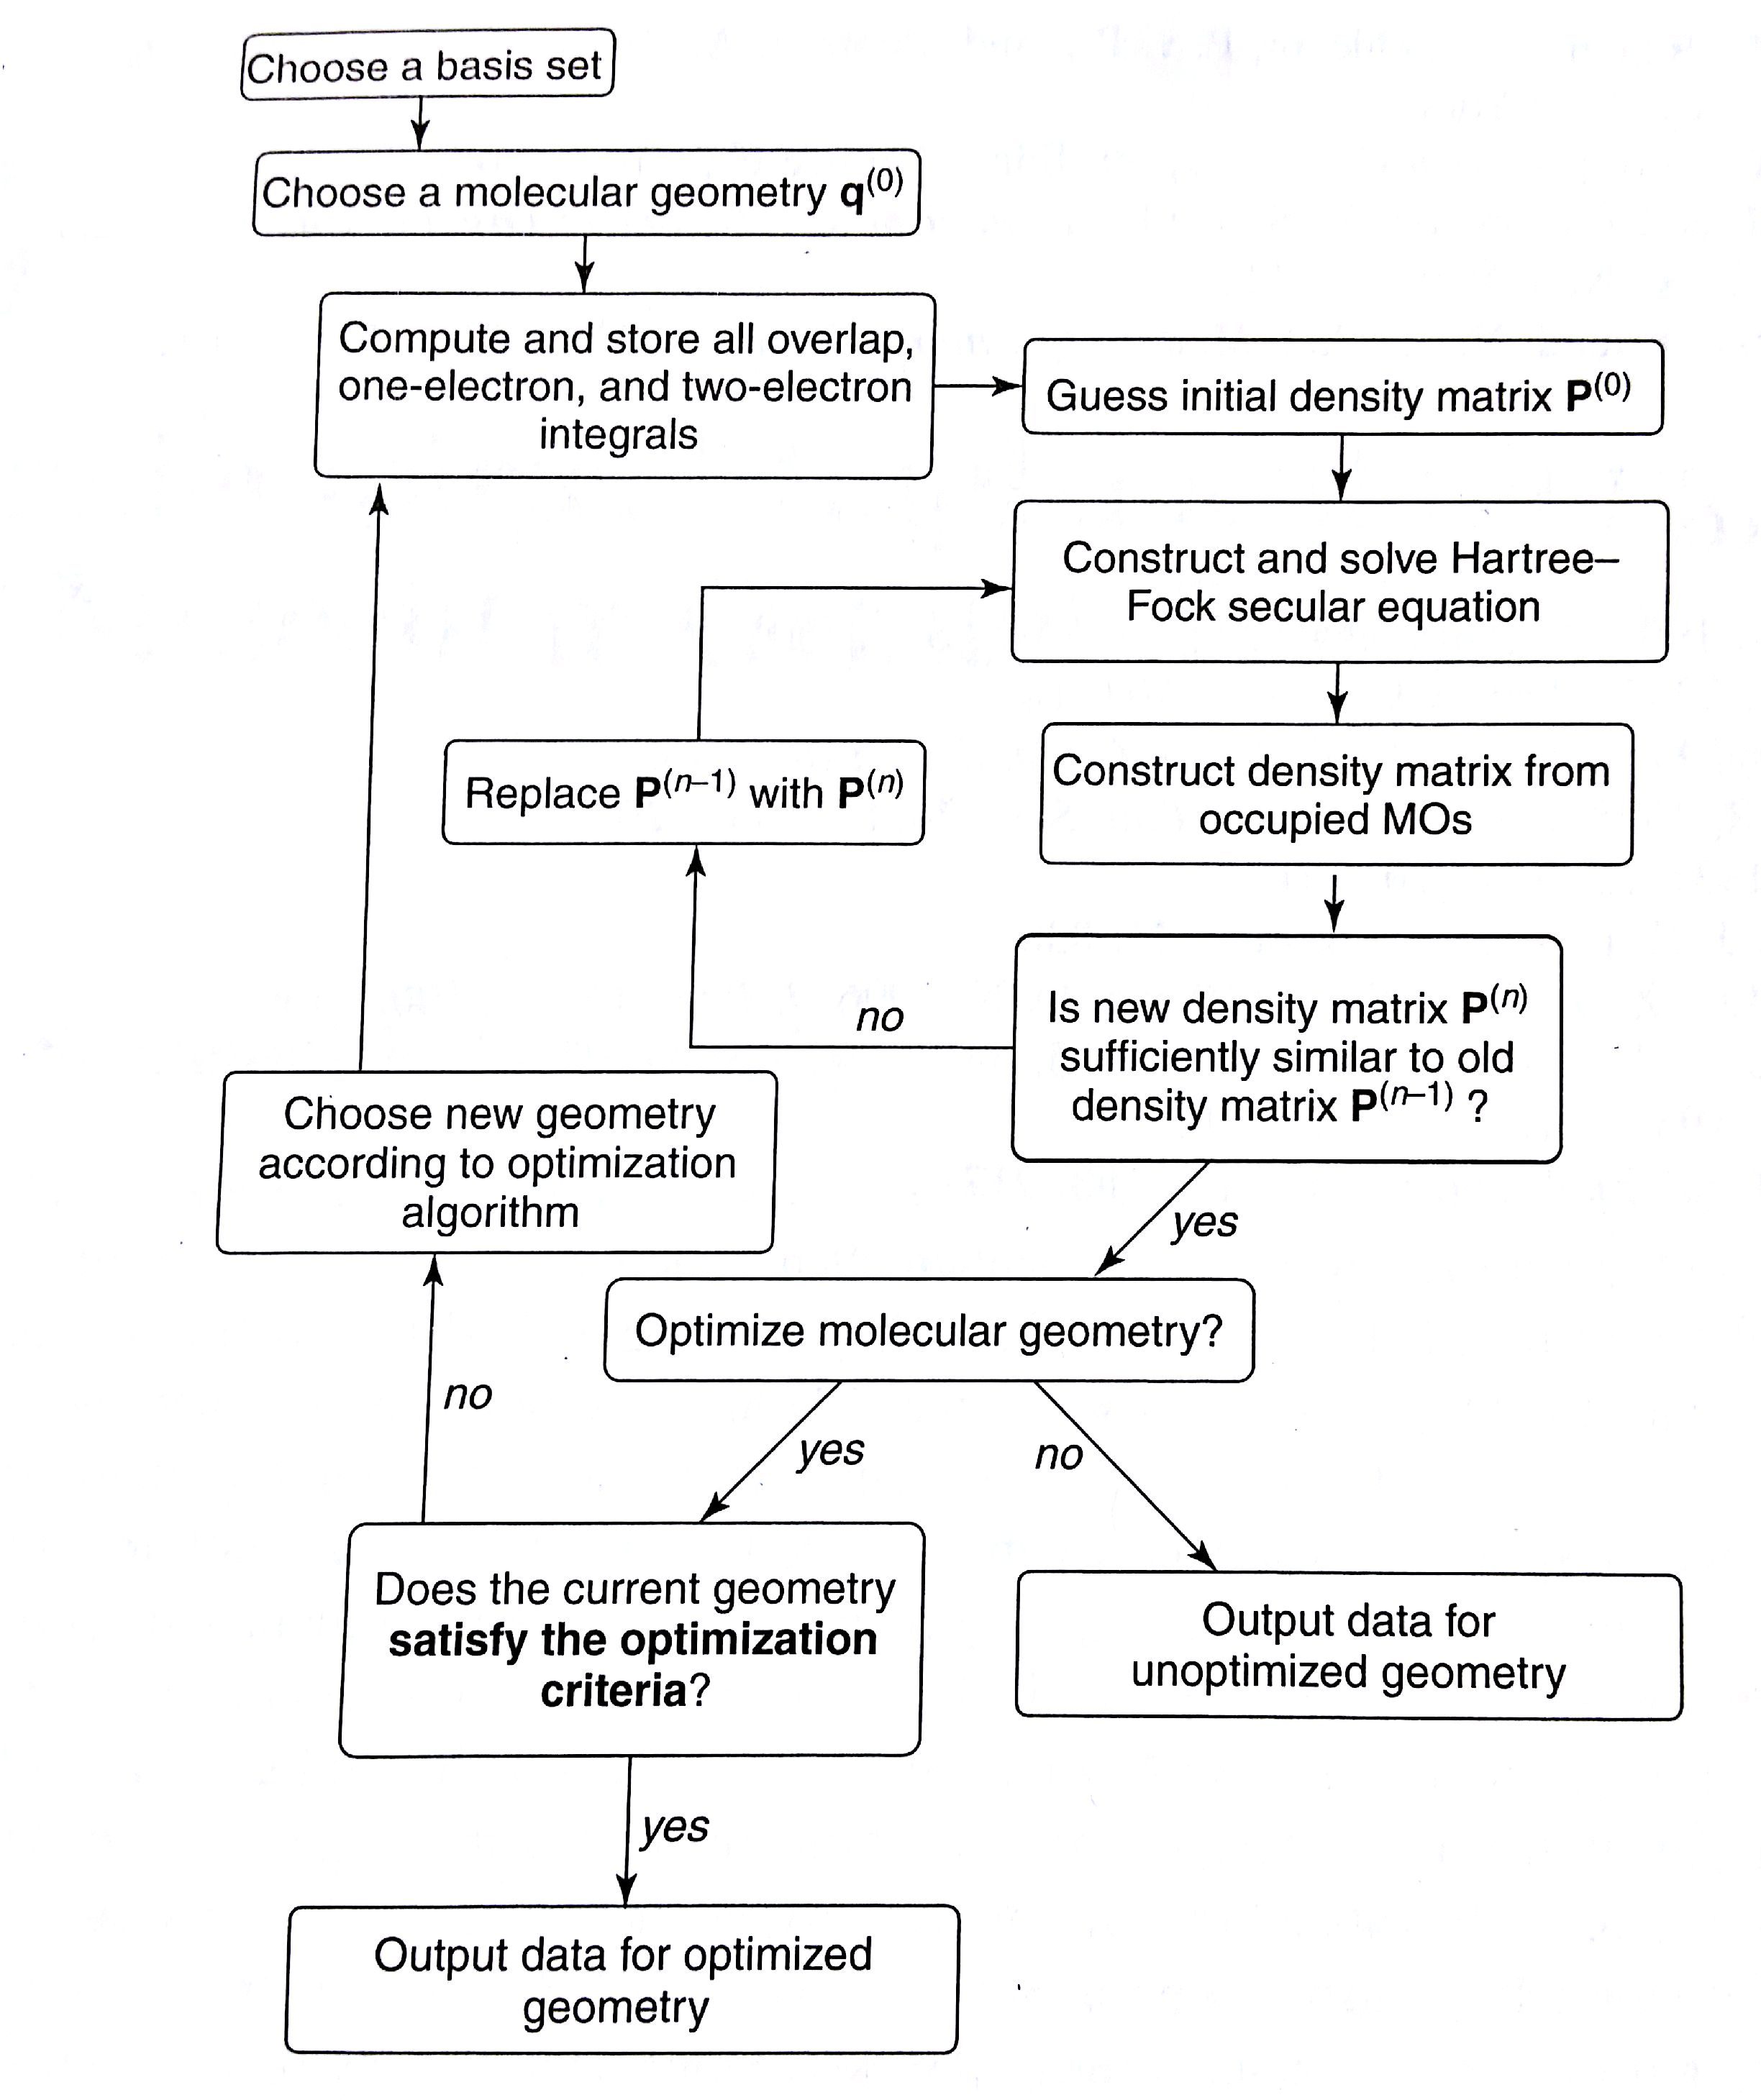
\includegraphics[scale=0.1,keepaspectratio]{Chapter-1/Figures/HFSCF.jpg}
                \caption{Flow chart of the HF SCF procedure}\label{fig:HF SCF flow chart}
            \end{figure}
            \fi

        The rest of this dissertation is organized as follows: Chapter 2 provides detailed information of the existing as well as novel methods, algorithms and techniques to compute quantum virial coefficients; Chapters 3 through 7 are each dedicated for a particular system (helium, hydrogen, nitrogen, oxygen and water respectively) and include motivation, recent developments, computational details, quantum virial coefficient results and discussion; Chapter 8 contains concluding remarks and future direction of work including some of the interesting challenges that are yet to be tackled.

\chapter{Methods}
\label{chap:methods}
\khExplicitPfalse
\graphicspath{{/home/ram/Desktop/Acads/Phd/dissertation/psuThesis/Chapter-2/Figures/}{/usr/users/rsubrama/Desktop/Acads/Phd/dissertation/psuThesis/Chapter-2/Figures/}}
    As mentioned in Sec. \ref{sec:chap1VirialCoefficients} the number of configuration integrals to be evaluated increases exponentially with the order of virial coefficient. In addition to that, the use of \abinitio{} potentials for quantum virial coefficient calculations involve siginificantly more computational effort than simple potential models. The need for such high quality virial coefficients, in order to predict accurate theromdynamic properties, should not be underestimated. Therefore efficient techniques are required in order to perform virial coefficient calculations. Graph theoretical methods were needed to represent the integrals as diagrams with a weight associated to it, especially for higher order coefficients, where writing out the integral would prove to be cumbersome. On the one hand, there have been theoretical methods \cite{Ree1964,Hellmann2011} developed to either reduce the number of these diagrams or combine them in a concise manner so as to improve the computational efficiency. On the other, computational techniques such as the VEGAS algorithm \cite{Lepage1972}, Mayer Sampling Monte Carlo (MSMC) \cite{Singh2004} and Wheatley's algorithm \cite{Wheatley2013} have also been developed to evaluate a given set of diagrams efficiently. The different theoretical methods and computational techniques complement each other very well and have made possible, for instance, the calculation of 16$^{\text{th}}$-order virial coefficents for the Lennard Jones model \cite{Feng2015}. Since the main aim of this work was to develop efficient methods, we shall restrict our attention to MSMC algorithm and the evaluation of second and third quantum virial coefficients for different systems. In that spirit, we present a brief summary of the MSMC algorithm in the following section.

\section{Mayer Sampling Monte Carlo}
    \label{sec:MSMC}
    \subsection{Introduction}
    \label{subsec:MSMCintro}
    MSMC is a free-energy perturbation technique which was developed by Singh and Kofke \cite{Singh2004} that involves avoiding the direct calculation of any desired integral (denoted as the `target') by computing its ratio to a known reference integral. The method uses importance sampling where the weight of a configuration is taken to be the absolute value of the integrand. Although it was developed originally using an umbrella-sampling \cite{Singh2004,Frenkel,Schultz2009} method, in its most recent form, the working equations of MSMC are cast using overlap-sampling method as:
    \begin{equation}
        \label{eq:MSMCworking}
        \begin{aligned}
            \Gamma (T) &= \Gamma_o \frac{{<\gamma/\pi>}_\pi / {<\gamma_{os}/\pi>}_\pi}{{<\gamma_o/\pi>}_{\pi_o} / {<\gamma_{os}/\pi_o>}_{\pi_o}}\\
            \gamma_{os} &= \frac{|\gamma_o||\gamma|}{\alpha |\gamma_o| + |\gamma|}
        \end{aligned}
    \end{equation}
    where $\Gamma (T)$ is the target integral, $\gamma$ is the target integrand, $\pi$ is the sampling weight of the target integrand, the subscript `$o$' denotes the corresponding quantities for the reference integral and integrands respectively, $\alpha$ is Bennett's \cite{Bennett1976} optimization parameter, and angular brackets $<\ldots>$ represent ensemble-averages.

    If computed directly, the target integral involves averaging lots of really large positive and negative numbers which could lead to imprecise results, especially for virial coefficient calculations \cite{Singh2004}. However, using MSMC this calculation is reduced to averaging the sign of the integrand because of the use of importance sampling, where we set $\pi = |\gamma|$. Thus, MSMC results in a more precise value than direct evaluation using numerical techniques. Additionally it is also computationally efficient than numerical techniques for higher order integrals. The versatility of the MSMC approach lies in the fact that it can be applicable to the evaluating of any integral irrespective of the its functional form (with a few caveats, for details see Ref. \cite{Singh2004}) with a whole variety of choices for the reference. For virial coefficient calculation purposes, $\Gamma$ is taken to be the configuration integral or sum of integrals. Singh and Kofke \cite{Singh2004} analyzed different options wih respect to calculating virial coefficents and suggested the use of hard-spheres as the reference for two reasons: 1) virial coefficients of hard spheres are temperature independent and 2) have been already evaluated precisely in literature. Highly precise and accurate virial coefficients of many systems including mixtures \hl{cite group papers here} have been successfully computed using MSMC, thus establishing a track-record of its performance. Hence, in all the computations performed related to this work, we have employed MSMC to compute virial coefficients efficiently.

    \subsection{Implementation}
    \label{subsec:MSMCimplementation}
        The idea behind this section is to outline some of the key features of a typical MSMC simulation that are common to all the systems, at the beginning, so that we need not repeat these for each type of system in later chapters. We may then focus on system-specific parameters within the `Computational details' section for each chapter. We provide details of how we collect data and our procedure to estimate the uncertainty as well.

        A typical MSMC simulation consists of two types of systems `target' and `reference'. Configurations are generated via MC trials for each system and are accepted/rejected with a probability $P_{\text{acc}}$:
        \begin{equation}
            \label{eq:MCacceptance}
            P_{\text{acc}} = \text{Min} \left(1, \displaystyle\frac{\pi^{\text{new}}}{\pi^{\text{old}}} \right)
        \end{equation}
        where $\pi$ is the sampling weight for that particular system, superscripts old and new are used to denote the old and new configurations respectively.

        Note that in Eq. \eqref{eq:MSMCworking}, ${<\gamma/\pi>}_\pi$ and ${<\gamma_{os}/\pi>}_\pi$ are called the target average and target-overlap average respctively. The corresponding terms for the reference system are called the reference average and the reference-overlap average respectively. In all MSMC simulations and for each system, molecule 0 always remains fixed at the origin and all MC trials generate configurations of the other molecules present in the system. A short equilibration simulation is performed at the beginning to determine $\alpha$ (Eq. \eqref{eq:MSMCworking}) and to adjust MC move step sizes so that the acceptance of all the MC moves is 50\%. Irrespective of their number, all MC moves are chosen with equal probability for both the systems within the simulation. After the equilibration period, we start collecting values of the reference, target, reference-overlap and target-overlap averages. The total number of configuration samples is divided into blocks of 1000 samples each. We compute averages of these four quantities and their standard deviation for each block. We then combine the averages across all blocks and use standard error formulas to estimate the overall value along with its standard deviations. The final values of virial coefficients and their standard deviations reported throughout this work are then obtained by using the reference, target, reference-overlap and target-overlap averages computed as mentioned above, Eq. \eqref{eq:MSMCworking} and simple error propagation formulas.

\section{Path Integrals}
    \subsection{Introduction}
        In this section we introduce the formalism developed by Richard Feynman \cite{Feynman} which provides guidelines for accounting nuclear quantum effects in quantum mechanical calculations. We do not attempt a fully rigorous mathematical re-derivation here but rather highlight some of they key aspects and formulas (from Feynman's book \cite{Feynman}) which are useful for the purpose of quantum virial coefficient calculations. For further details, the interested reader may refer Refs. \hl{PI references}. Primarily, the purpose of this section is to establish a relationship between the thermal density matrix which is derived from statistical mechanics and the kernel of the wave function derived from the \Schrodinger{} equation. Thus creating the important link between microscopic states and macroscopic observables.

        The advent of quantum mechanics in the 1920s brought about a fundamentally new way of thinking about relativistic particles. The classical definitions of probability due to Laplace could no longer be applicable for systems of extremely small sizes. Note that what had changed was not the idea or concept of probability but rather the prescribed way of computing it. Different physicists proposed different hypotheses for computing the probability according to quantum mechanics.

        Feynman's Path Integral (PI) formalism has at its beginning stages, simple probability definitions associated with events for a relativistic particle such as the electron. One important idea was to associate a complex amplitude ($\phi(x)$) with the probability of an event $P$ depending on some variable $x$, such that $P = |\phi(x)|^2$. Since there could be many possible ways for the event to happen, we associate an amplitude to each such alternative and compute the overall probability as $P = |\Phi(x)|^2; \Phi(x) = \phi_1(x) + \phi_2(x) + \cdots$. Similarly, expressions for events occuring in succession, mutually exclusive events and various other definitions corresponding to classical probability, can be obtained. Starting with these basic definitions, for each path or trajectory associated with the movement of a particle, a contribution to the probability amplitude was associated. Therefore, we could define a quantity called `kernel' that represented the sum of contributions from each possible path. The action $S$ associated with a particle of mass $m$ traveling in a potential $V(x,t)$ is given in terms of its Lagrangian $L$ as:
        \begin{equation}
        \label{eq:action}
            \begin{aligned}
                S &= \displaystyle \int_{t_a}^{t_b} L(\dot{x},x,t) dt,\\
                L(\dot{x},x,t) &= \frac{m{\dot{x}}^2}{2} - V(x,t).
            \end{aligned}
        \end{equation}

        Whereas only the path with the least action contributes to the classical trajectory, all paths contribute equally to the quantum trajectory and do so in different phases. This was another important idea that was employed in the development of PI formalism. Based on the above definitions, we can calculate the probability associated with the movement of a particle from point $a$ to $b$:
        \begin{equation}
        \label{eq:quantum probability}
            \begin{aligned}
                \phi(x,t) &= \text{const.} e^{iS[x(t)]/\hbar},\\
                \Rightarrow K[b,a] &= \displaystyle\sum\limits_{\text{all paths}} \phi[x(t)],\\
                P(b,a) &= {|K[b,a]|}^2.
            \end{aligned}
        \end{equation}
        where $K[b,a]$ is the kernel.

        Consider a particle of mass $m$ traveling in a potential $V(x,t)$, with action defined as in Eq. \eqref{eq:action}. We can construct the ``path integral'' analogous to the Riemann integral:
        \begin{equation}
            \begin{aligned}
                K[b,a] &= \displaystyle\lim_{\epsilon\,\to\ 0} \frac{1}{A}\int_{-\infty}^\infty\,\int_{-\infty}^\infty\,\cdots\,\int_{-\infty}^\infty e^{\frac{iS[b,a]}{\hbar}}\,\frac{dx_1}{A}\,\frac{dx_2}{A}\ldots\,\frac{dx_{N-1}}{A},\\
                A &= {\left( \displaystyle\frac{2\pi i \hbar \epsilon}{m} \right)}^{\frac{1}{2}}.
            \end{aligned}
        \end{equation}
        More compactly, it can be written in terms of the new path integral notation $\mc{D} x(t)$ as:
        \begin{equation}
        \label{eq:PI compact kernel}
            K[b,a] = \displaystyle \int_{a}^b e^{\frac{iS[b,a]}{\hbar}} \mc{D} x(t).
        \end{equation}
        For a more general case of having $N-1$ intermediate points between $a$ and $b$, the kernel is given as:
        \begin{equation}
            \begin{aligned}
                K[b,a] = \int_{x_{N-1}}\,\cdots\,\int_{x_2}\,\int_{x_1} &K[b,N-1]K[N-1,N-2]\,\ldots\\
                & \qquad K[i+1,i] \ldots K[1,a]\,dx_1\,dx_2\ldots dx_{N-1}
            \end{aligned}
        \end{equation}
        
        \subsubsection{Kernel of the Wave Function}
            Assume that the amplitude to arrive at any point $b = (x,t)$ irrespective of the starting point $a$, to be given by $\psi (x,t)$. It can be shown that $\psi (x,t)$ also has the same probability charecteristics as the kernel, i.e., $P = |\psi (x,t)|^2$ and we call $\psi (x,t)$ the wave function. Based on this definition, we could compute the wavefunction exactly at any future point if we know its exact value at any time $t$.

            The \Schrodinger{} equation is solvable by separation of variables in the speical case where we use a time-indpendent Hamiltonian:
            \begin{equation}
                \label{eq:psi}
                \begin{aligned}
                    \psi(x,t) &= \phi(x)e^{(-i/\hbar)Et},\\
                    \mc{H} \phi(x) &= E \phi(x).
                \end{aligned}
            \end{equation}

            Using orthonormal basis functions to represent $\psi(x,t)$ and given $t_b > t_a$, the kernel is given by:
            \begin{equation}
                \label{eq:kpsi}
                K[x_b,t_b;x_a,t_a] = \displaystyle\sum\limits_{n = 1}^\infty \phi_n(x_b){\phi^*_n(x_a)} e^{(-i/\hbar)E_n(t_b - t_a)}
            \end{equation}
            where $\phi^*(x)$ denotes the complex conjugate of the $\phi(x)$ and $E_n$ are the eigenvalues of Eq. \eqref{eq:psi}. It can be shown that the kernal in Eq. \eqref{eq:kpsi} also satisfies the \Schrodinger{} equation.

        \subsubsection{Thermal Density Matrix}
            From statistical mechanics, we know that at thermal equilibrium at a temperature $T$, the probability that a system exists in a state with energy $E$ is proportional to the Boltzmann factor $e^{-\beta E}$. Here $\beta = 1/k_\text{B} T$ and $k_\text{B}$ is the Boltzmann constant. Assuming non-degenerate states, the normalized probability distribution is given by:
            \begin{equation}
                \begin{aligned}
                    p_n &= \frac{1}{Z}e^{-\beta E_n}, \\
                    Z &= \displaystyle\sum\limits_n e^{-\beta E_n}.
                \end{aligned}
            \end{equation}
            
            Suppose 'A' is some property of interest, its mean value in the $n^{th}$ energy state and the corresponding statistical average for the whole system are computed as:
            \begin{equation}
                \begin{aligned}
                    A_n &= \displaystyle\int \phi_n^* A \phi_n d\Gamma,\\
                    \bar{A} &= \displaystyle\sum\limits_n p_n A_n = \frac{1}{Z} \displaystyle\sum\limits_n A_n e^{-\beta E_n}.
                \end{aligned}
            \end{equation}
            where $\Gamma$ denotes the configuration space and integral over $\Gamma$, the configurational integral.

            If the system exists in a single state defined by the wavefunction $\phi_n(x)$, the probability of observing it and the expectation value can be calculated as: 
            \begin{equation}
                \label{eq:prob stat mech}
                \begin{aligned}
                    P(x) &= \displaystyle\sum\limits_n \phi_n^*(x) \phi_n(x) e^{-\beta E_n}\\
                    \bar{A} &= \displaystyle \frac{1}{Z} \displaystyle\sum\limits_n A_n e^{-\beta E_n} = \frac{1}{Z} \displaystyle\sum\limits_n \int \phi_n^*(x) A \phi_n(x)\: e^{-\beta E_n} dx
                \end{aligned}
            \end{equation}

            We can calculate the expected value of any quantity A using if we know the function:
            \begin{equation}
                \label{eq:rho stat mech}
                \rho(x',x) = \displaystyle \sum\limits_n \phi_n(x') \phi_n^*(x) e^{-\beta E_n}
            \end{equation}
            
            From Eqs. \eqref{eq:prob stat mech} and \eqref{eq:rho stat mech}, we can write down the expression for the partition function $Z$ as:
            \begin{equation}
                \begin{aligned}
                    P(x) &= \frac{1}{Z} \rho(x,x),\\
                    Z &= \int \rho(x,x) dx \equiv \text{trace} \{\rho\}.
                \end{aligned}
            \end{equation}
            where $\rho(x',x)$ is called the statistical thermal density matrix at temperature T.
            
            Comparing the expressions for the kernel (Eq. \eqref{eq:kpsi}) and the density matrix (Eq. \eqref{eq:rho stat mech}), we see that if we replace `$t_b - t_a$' of Eq. \eqref{eq:kpsi} with `$-i \beta \hbar$' , the resulting expressions are identical. Therefore we can write:
            \begin{equation}
                \rho (x_b, x_a; \tau) = \displaystyle \int exp \left\{ - \frac{1}{\hbar} \: \int_0^{\tau} \left[ \frac{m}{2} {\dot{x}(u)}^2 + V(x(u)) \right] du \right\} \mc{D}x(u)
            \end{equation}
            where $\tau = \beta \hbar$, has units of time and this led to the often used expression `imaginary-time' path integrals. 
            
    \subsection{Path Integral Monte Carlo}
        The thermal density matrix $\rho$ plays a key role in Feynman's imaginary-time PI formalism and its application in Monte Carlo (MC) algorithms to compute physical properties of interest. In position space, it is given by \cite{Feynman,Ceperley1995,Cui1997}:
        \begin{equation}\label{eq:rho}
            \rho (R , R' ; \beta) = < R | e^{- \beta \ham{H} } | R' >
        \end{equation}
        where $R = \{\bm{r}_1, \bm{r}_2, \ldots \bm{r}_n\}$ and $\beta = 1/k_{\rm B}T$, with $k_{\rm B}$ Boltzmann's constant and $T$ the temperature. A key property of the density matrix is that the product of two density matrices is also a density matrix:
        \begin{equation}\label{eq:dmProduct}
            \rho (R, R'; \beta_1) \times \rho (R, R'; \beta_2) = \rho (R, R'; \beta_1 + \beta_2)
        \end{equation}
        This is because any operator (specifically the Hamiltonian operator \ham{H} here) is commutative with any scalar multiple of itself. This exact property allows us to write down the following $(P-1)$-fold convolution:
        \begin{equation}\label{eq:convolution}
            \rho (R_0, R_P; \beta) = \displaystyle\int \cdots \int dR_1 \, dR_2 \, \ldots \, dR_{P-1} \: \rho (R_0, R_1; \tau) \rho (R_1, R_2; \tau) \ldots \rho (R_{P-1}, R_P; \tau)
        \end{equation}
        where $\tau = \beta/P$. Note that even though the above expression is exact, one needs to make approximations to the thermal density matrix in order to compute the convolution efficiently. The simplest of the approximations is to assume that the kinetic-energy operator (\ham{T}) and the potential-energy operator (\ham{V}) in the Hamiltonian commute with each other. As $\tau \to 0$ or equivalently as $PT \to \infty$, the ``primitive approximation'' is given by:
        \begin{equation}\label{eq:primitiveApprox}
            e^{- \tau (\ham{T} + \ham{V})} \approx e^{- \tau \ham{T}} e^{- \tau \ham{V}}
        \end{equation}
        The Trotter formula proves that this approximation does converge to the right result in the $P \to \infty$ limit and is given by:
        \begin{equation}\label{eq:trotter}
            e^{- \beta (\ham{T} + \ham{V})} = \lim_{P \to \infty} \Big[ e^{- \tau \ham{T}} e^{- \tau \ham{V}} \Big]^P
        \end{equation}

        \subsubsection{Fully Quantum Second Virial Coefficients}
            In this section we provide expressions (without going into too much mathematical detail, for further information see Refs. \cite{Cui1997,Patkowski2008,Garberoglio2009,Garberoglio2014}) for the fully quantum virial coefficients, first for the case of a diatomic rigid rotor. The expression for the monatomic molecule can then be obtained simply by ignoring the terms related to the orientational degrees of freedom in it.

            Let $m$ and $I$ denote the mass of the atom and moment of interia of the rigid rotor respectively with $\Lambda_m = h/\sqrt{2\pi m k_B T}$. Its Hamiltonian is given by:
            \begin{equation}
            \label{eq:hDiatomic}
                \hat{h}_2 = \displaystyle\frac{\hat{\mbf{p}}^2}{2m} + \frac{\hat{\mbf{J}}_1^2}{2I} + \frac{\hat{\mbf{J}}_2^2}{2I} + \hat{U}(r,\Omega_1,\Omega_2)
            \end{equation}
            where $\hat{\mbf{p}}$ is the momentum operator conjugated to the COM separation, $\hat{\mbf{J}}_1$ and $\hat{\mbf{J}}_2$ are the angular momentum operators, $\hat{U}(r,\Omega_1,\Omega_2)$ is the intermolecular potential function in terms of the COM distance $r$ and the orientation vectors $\Omega_1$ and $\Omega_2$.

            Note that because the momentum operator is conjugated to the COM separation, we can use the set of vectors $\mbf{x}^i,\mbf{\Omega}_1^i, \mbf{\Omega}_2^i$ to denote the configuration of the two $i^\text{th}$ rigid rotors. Employing the primitive approximation (Eq. \eqref{eq:primitiveApprox}) to the diatomic Hamiltonian and using the Trotter formula \ref{eq:trotter}, we get \cite{Cui1997}:
            \begin{equation}
                \begin{aligned}
                    \left< \mbf{x}^i \left| \exp \left(-\displaystyle\frac{\beta \hat{\mbf{p}}^2}{2 m P} \right) \right| \mbf{x}^{i+1} \right> &= \displaystyle\frac{P^{3/2}}{\Lambda^3} \exp \left(-\displaystyle\frac{\pi P (\mbf{x}^i - \mbf{x}^{i+1})^2}{\Lambda_m^2}\right)\\
                    \left< \Omega^i \left| \exp \left(-\displaystyle\frac{\beta \hat{\mbf{J}}^2}{2IP} \right) \right| \Omega^{i+1} \right> &= \displaystyle\sum_{j=0}^\infty \frac{2j+1}{4 \pi} \mc{P}_j (cos (\theta_{i,i+1}))\nonumber \exp \left[-\beta j(j+1) \Upsilon/ P \right]
                \end{aligned}
            \end{equation}
            where $j$ is the angular quantum number, $\theta_{i,i+1}$ is the angle between bead orientation vectors $\Omega_i, \Omega_{i+1}$ and $\mc{P}_j$ is the Legendre polynomial of order $j$.

            Defining $\mbf{r} \equiv \mbf{x}^{(1)}, \mbf{\Delta}^{(i)} \equiv \mbf{x}^{(i+1)} - \mbf{x}^{(i)}$ and $\bar{U}$ as:
            \begin{equation}
                \label{eq:uBarDiatomic}
                \exp [-\beta \bar{U} (|\mbf{r}|) = \left< \exp \left[ -\displaystyle\frac{\beta}{P} \sum_{i=1}^P U (|\mbf{x}^i|,\Omega_1^i,\Omega_2^i) \right] \right>_{F,\varrho}
            \end{equation}
            where $<\cdots>_{F,\varrho}$ denotes the ensemble average over ring polymer conformations $\mbf{\Delta}$ and rotor orientations $\mbf{\Omega}_1$ and $\mbf{\Omega}_2$ sampled according to the distributions $F$ and $\varrho$ defined below:
            \begin{subequations}
                \begin{align}
                    F(\mbf{\Delta}) &= \Lambda_m^3 { \left( \frac{P^{3/2}}{\Lambda_m^3} \right)}^P \exp \left( - \frac{\pi P}{\Lambda_m^2} \displaystyle\sum\limits_{i=1}^P {|\mbf{\Delta}^{(i)}|}^2 \right)\label{eq:fRingDiatomic}\\
                    \varrho(\mbf{\Omega}) &= \frac{1}{q_{rot}} \displaystyle\prod_{i=1}^P \sum_{j=0}^\infty \frac{2j+1}{4 \pi} \mc{P}_j (cos (\theta_{i,i+1})) \exp \left[-\beta j(j+1) \Upsilon/ P \right],\label{eq:rhoDiatomic}\\
                    q_{rot} &= \displaystyle\sum_{l} (2l + 1) \exp \left[-\beta \Upsilon l (l+1) \right],\nonumber\\
                    \Upsilon &= \displaystyle\frac{\hbar^2}{2I}\nonumber.
                \end{align}
            \end{subequations}

            The fully quantum second virial coefficient based on $\bar{U} (r)$ (Eq. \eqref{eq:uBarDiatomic}), for a diatomic molecule is given by:
            \begin{equation}
            \label{eq:b2Diatomic}
                B_2 (T) = -2 \pi \displaystyle\int dr~ r^2 (e^{-\beta \bar{U} (r)} - 1)
            \end{equation}

            To obtain the the expression for the case of the monatomic molecule, we simply ignore all the orientation related terms to obtain:
            \begin{equation}
                \label{eq:uBarMonatomic}
                \exp [-\beta \bar{U} (|\mbf{r}|) = \left< \exp \left[ -\displaystyle\frac{\beta}{P} \sum_{i=1}^P U (|\mbf{x}^i|) \right] \right>_F
            \end{equation}
            where $<\cdots>_F$ denotes the ensemble average over ring polymer conformations $\mbf{\Delta}$ sampled according to the distribution $F$ (Eq. \eqref{eq:fRingDiatomic}).
            
            The fully quantum second virial coefficient based on $\bar{U} (r)$ (Eq. \eqref{eq:uBarMonatomic}), for a monatomic molecule is given by:
            \begin{equation}
            \label{eq:b2Monatomic}
                B_2 (T) = -2 \pi \displaystyle\int dr~ r^2 (e^{-\beta \bar{U} (r)} - 1)
            \end{equation}

            Note that the distribution $F$ (Eq. \eqref{eq:fRingDiatomic}) for sampling $\mbf{\Delta}$ conformations or equivalently the internal bead positions, is the same for both the diatomic as well as the monatomic cases.

    \subsection{PIMC With Semi-classical Beads}
    \label{chap:methods:subsec:PI SCB}

        It is worth noting that within the PI implementation, we are mainly interested in evaluating the trace of the density matrix, as it is directly related to the partition function. Also when using the primitive approximation, we neglect terms that are of the order $\tau^2$. To improve the precision of results in MC simulations and to achieve faster convergence as $P$ increases, higher order corrections (or propagators of the density matrix) have been developed. The Takahashi-Imada (TI) propagator \cite{Takahashi1984} with error of the order $\tau^4$ uses:
        \begin{equation}\label{eq:TI}
            \begin{aligned}
                Tr \Big[ e^{- \beta ( \ham{T} + \ham{V} )} \Big] &= Tr \Big[ e^{ -\frac{\beta}{P} \ham{T}} e^{-\frac{\beta}{P} \mc{V'}} \Big]^P + O (\beta^5 P^{-4}),\\
                \mc{V'} &= \ham{V} + \frac{1}{24} \bigg( \frac{\beta}{P} \bigg)^2 [\ham{V}, [\ham{T}, \ham{V}]].
            \end{aligned}
        \end{equation}
        Given a system with Hamiltonian \ham{H} as:
        \begin{equation}\label{eq:h}
            \begin{aligned}
                \ham{H} &= \ham{T} + \ham{V},\\
                \ham{T} &= -\displaystyle\frac{\hbar^2}{2m} \sum\limits_{i=1}^N \frac{\partial^2}{\partial \bm{r}_i^2},\\
                \ham{V} &= V (\bm{r}_1, \ldots , \bm{r}_N),
            \end{aligned}
        \end{equation}
        it can be easily shown that from Eqs. \eqref{eq:TI} and \eqref{eq:h}, we get the following:
        \begin{equation}\label{eq:TIworking}
            \mc{V'} = V (\bm{r}_1, \ldots ,\bm{r}_N) + \frac{\hbar^2}{24m} \bigg(\frac{\beta}{P} \bigg)^2 \displaystyle\sum\limits_{i=1}^N \big|\pmb{\nabla}_i V (\bm{r}_1, \ldots ,\bm{r}_N) \big|^2,
        \end{equation}
        where $\hbar$ is the reduced Planck's constant and $\pmb{\nabla}_i$ denotes the gradient with respect to coordinates of the $i^{th}$ atom. Equations \eqref{eq:TI} and \eqref{eq:TIworking} constitute the working equations of the the TI propagator. Schenter \cite{Schenter2002} computed fully quantum virial coefficients using three different interaction potentials for water and found that using the semi-classical TI approximation (Eq. \eqref{eq:TIworking} with $P = 1$) gave the best agreement to fully quantum statistical mechanical calculations, especially at low temperatures where conventional expressions (based on the primitive approximation) including first order quantum corrections failed.

        Janke and Sauer~\cite{Janke1992} showed that by adopting a slightly modified version of the Trotter formula (Eq.~\eqref{eq:trotter}), they could systematically decrease the variance of the propagator. By decomposing the Hamiltonian to include more and more components of the kinetic- and potential-energy operators, they observed that the variance of the propagator improved.

        Suzuki \cite{Suzuki1995} suggested new schemes for the exponential product formulae along with a basic theorem for a generalized decomposition that results in the propagator having error of the order $O(1/P^4)$. Yamamoto \cite{Yamamoto2005} showed that using a finite-difference based approach (instead of computing derivatives involved with the use of TI and Suzuki propagators) helped improve the variance further.
        
        Apart from the propagators mentioned above, statistical estimators of the total energy with low variances have also been developed. We mention them here in passing without going into too much detail. The Barker or the thermodynamic estimator\cite{Barker1979} ($\epsilon_T$) is obtained by the direct differentiation of the partition function with temperature. It can be easily derived starting from a Hamiltonian of the form given in Eq. \eqref{eq:h} and is given as:
        \begin{equation}\label{eT}
            \begin{aligned}
                E(\beta) &= - \displaystyle\frac{1}{Z(\beta)} \frac{\partial Z(\beta)}{\partial \beta} \approx <\epsilon_T>\\
                \epsilon_T &= \displaystyle\frac{3P}{2\beta} - \frac{mP}{2\hbar^2 \beta^2} \sum\limits_{s=1}^P (x_s - x_{s-1})^2 + \frac{1}{P} \sum\limits_{s=1}^P V(x_s)
            \end{aligned}
        \end{equation}

        The Berne virial estimator\cite{Cao1989} ($\epsilon_V$) is a modification of the Barker estimator that eliminates ill-behaved terms  as $P \to \infty$. $\epsilon_V$ is given as:
        \begin{equation}\label{eV}
            \begin{aligned}
                \epsilon_V &= \displaystyle\frac{3g}{2\beta} + \frac{1}{P} \sum\limits_{s=1}^P \bigg[ V(x_s) + \frac{1}{2} (x_s - x^*) \frac{\partial V(x_s)}{\partial x_s} \bigg]\\
                x^* &= 0\: \: \text{or}\:\: x_P \: \:\text{or} \:\: x_C\\
                g &= 0 ~\text{if}~ x^* = 0~ \text{else}~ g = 1
            \end{aligned}
        \end{equation}
        where $\epsilon_V$ is called the origin-, bead- and centroid-reference virial estimator for $x^* = 0, x_P$ and $x_C$ respectively.

        The variance of the centroid virial estimator is weakly dependent on $P$ whereas the variance of the Barker estimator is directly proportional to $P$\cite{Cao1989}. This leads to faster convergence and lower uncertainties as $P \to \infty$ and therefore the centroid virial estimator is generally considered better than the Barker estimator. Berne and Cao\cite{Cao1989} showed that the variance of the virial estimator is also affected by the MC algorithm that was being used, comparing the performance of the virial estimator for four different MC algorithms. Glaesemann and Fried\cite{Glaesemann2002} reported an improved thermodynamic estimator based on a free particle projection with variance similar to that of the virial estimator. One of the advantages of this estimator is that it requires one fewer derivative compared to its virial counterpart.

        The kinetic-energy operator in the Hamiltonian gives rise to the weight of the ring configuration, which depends on the harmonic energy of the system with $P$ beads. The potential-energy operator (and hence, the \abinitio{} PES leads to the effective potential $\bar{U} (r)$ in the expressions for the quantum second virial coefficient (Eqs. \eqref{eq:b2Monatomic} and \eqref{eq:b2Diatomic} for the monatomic and diatomic cases respectively). Recall that we used the primitive approximation where the potential-energy operator was a simple function of the PES. If instead, we were to include higher order terms in the primitive approximation using the TI propagator, we would expect it to affect only $\bar{U} (r)$ (Eq. \eqref{eq:uBarMonatomic} and \eqref{eq:uBarDiatomic} for the monatomic and diatomic cases respectively). Thus using the TI propagator is equivalent to computing $\bar{U} (r)$ (Eq. \eqref{eq:uBarMonatomic} and \eqref{eq:uBarDiatomic} for the monatomic and diatomic cases respectively) using $\mc{V'}$ (Eq. \eqref{eq:TIworking}).

        We can see that the argument within the sum on the right-hand side of the expression for $\bar{U} (r)$ (Eqs. \eqref{eq:uBarMonatomic} and \eqref{eq:uBarDiatomic}) goes from being a quantity completely independent of $P$ and $\hbar$ while using the primitive approximation, to a quantity that is dependent on both $P$ and $\hbar$ while using the TI propagator and Eq. \eqref{eq:TIworking}. The inter-molecular potential experienced by the beads of the ring changes from being classical to semi-classical (dependent on $P$ and $\hbar$). Therefore, the phrase `PIMC with \textbf{semi-classical beads}' along with Fig. \ref{quantumness} is an apt description of such a PIMC simulation. For a fixed $P$, we would expect to capture more quantum effects with the use of semi-classical beads than classical beads, that is, by using the primitive approximation with higher order terms than just the primitive approximation by itself.
        \begin{figure}
            \centering
            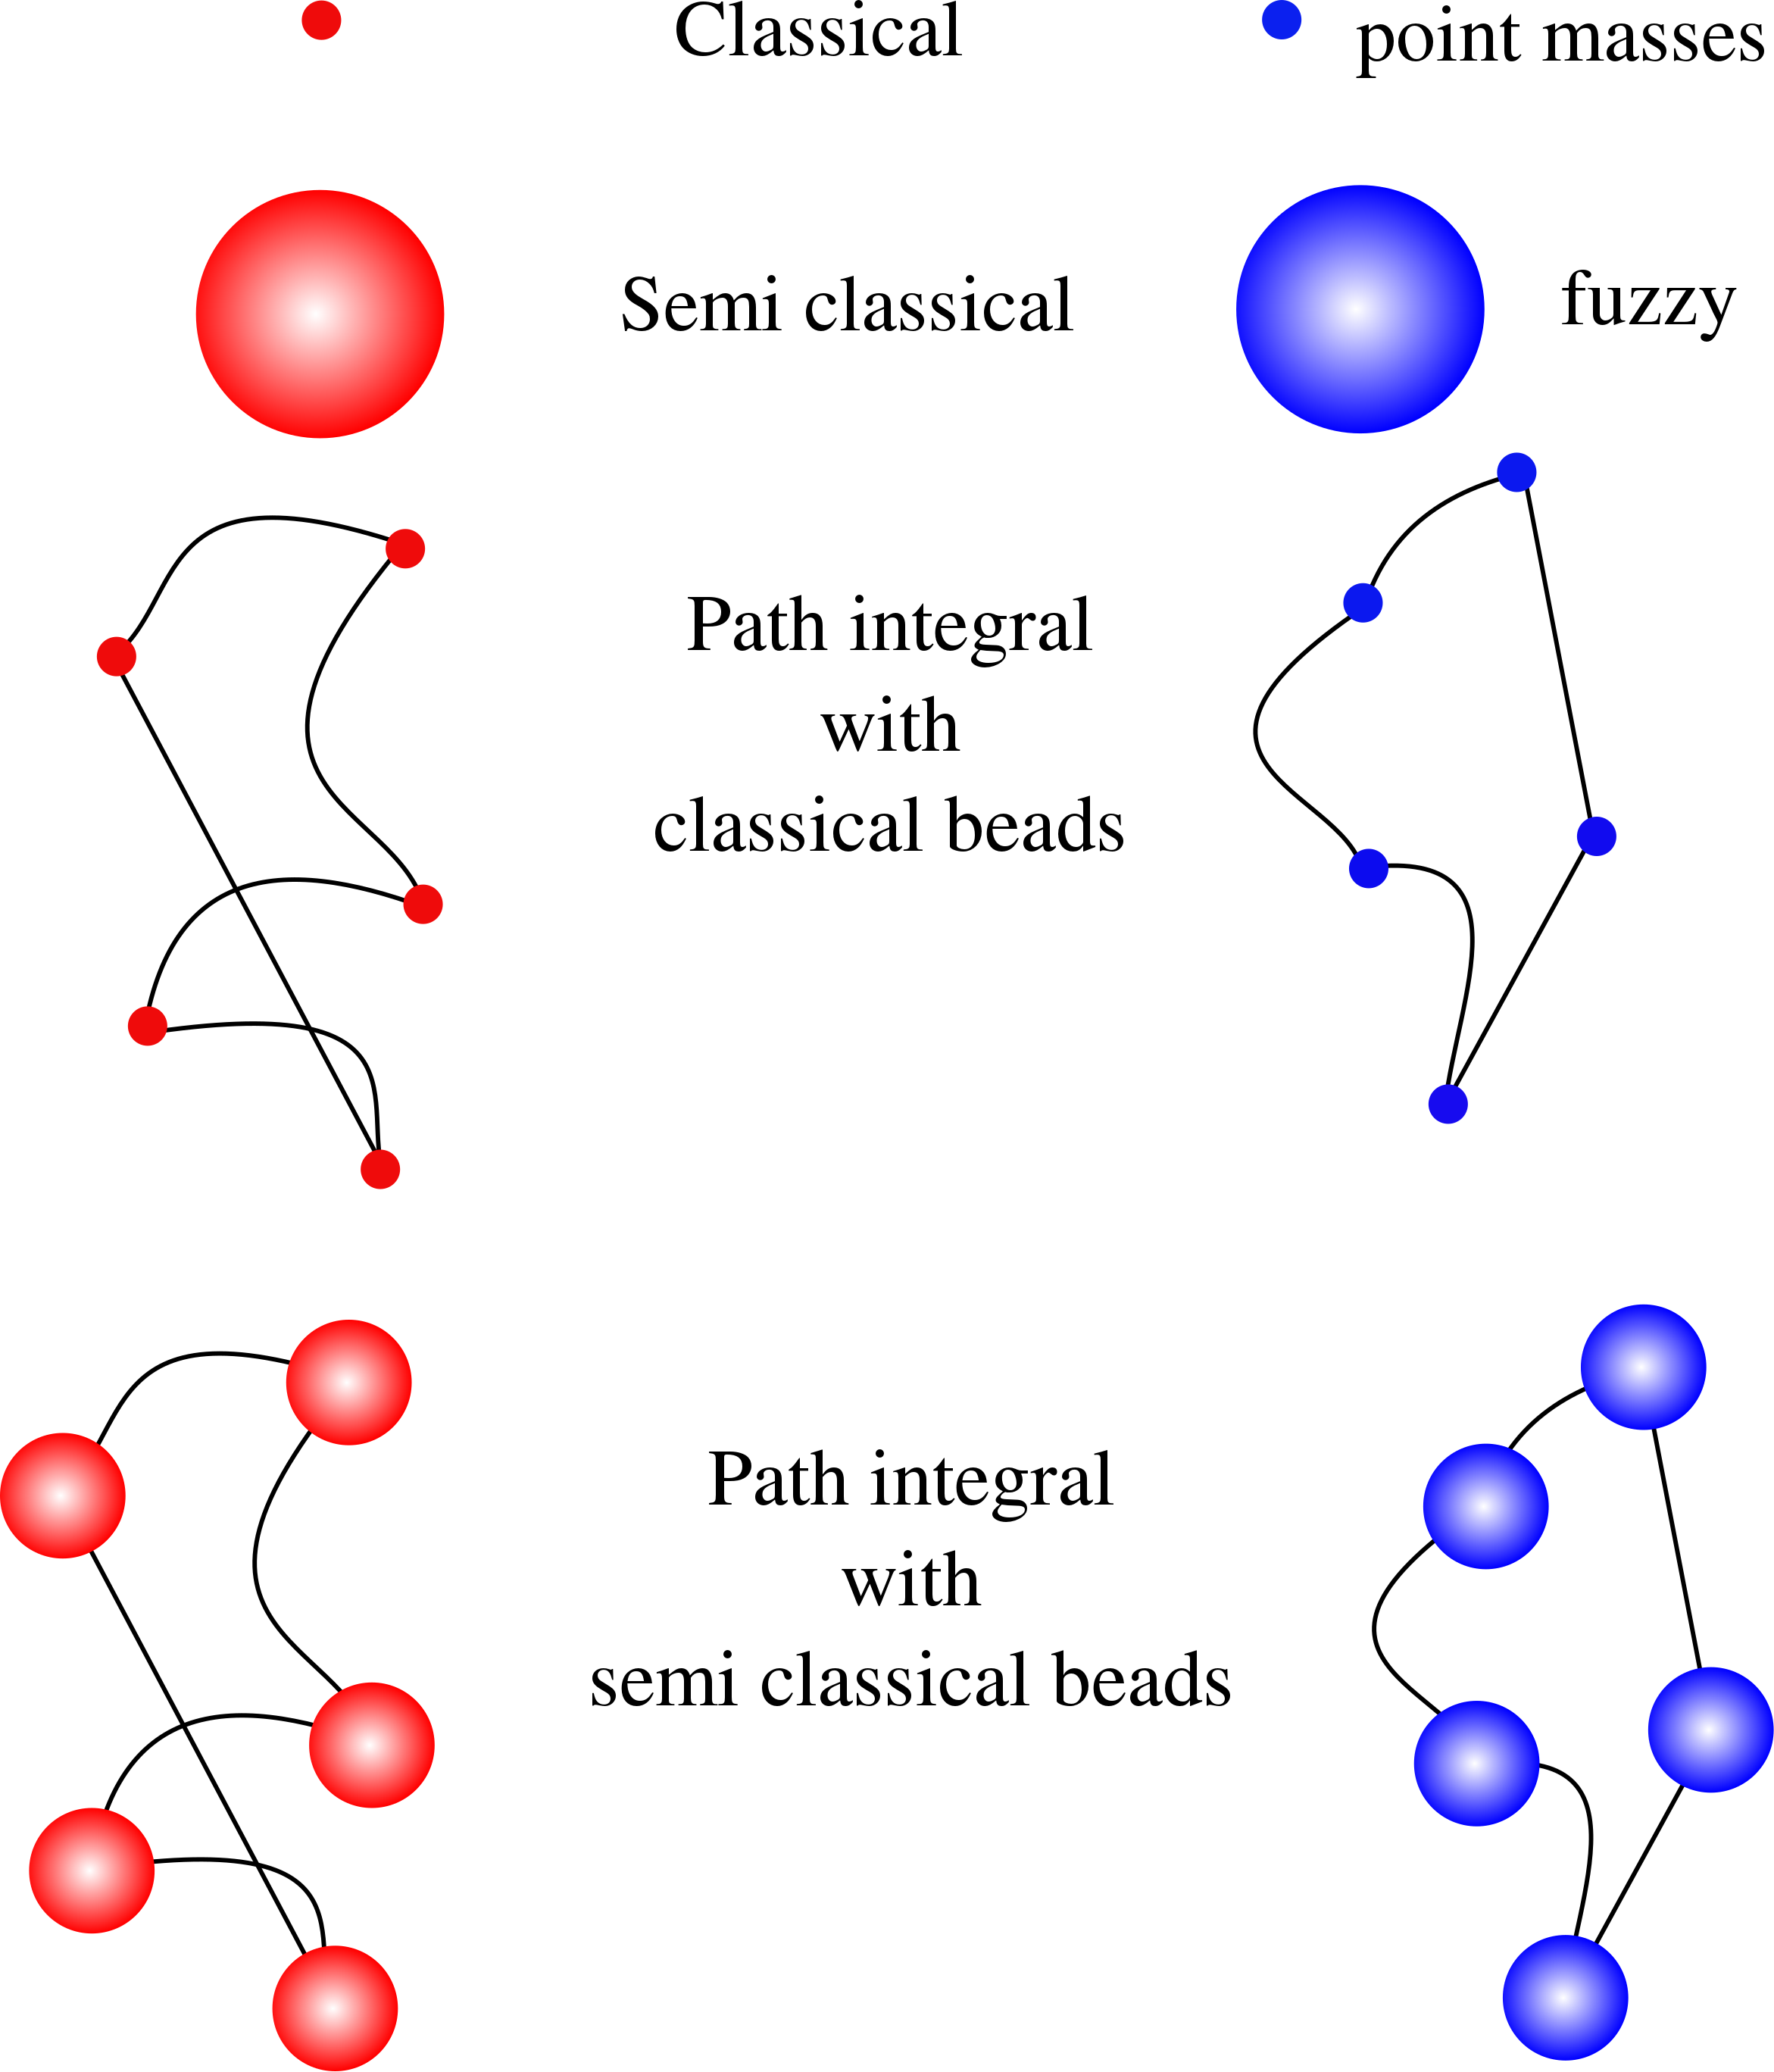
\includegraphics[scale=0.087,keepaspectratio]{quantumLevels.png}
            \caption{Different levels of ``quantumness'' of a $B_2$ calculation going from classical virial coefficients that are calculated assuming point masses to fully quantum virial coefficients with semi-classical beads. The different sphere sizes here are for illustrative purposes only and no quantitative inference should be made.} \label{quantumness}
        \end{figure}
        
        We summarize here the equations pertaining to PIMC calculations with semi-classical beads (SCB) based approach using the TI propagator.
        The fully quantum second virial coefficient expression using SCB-TI approach is given by:
        \begin{equation}
        \label{eq:b2SCBTI}
            B_2 (T) = -2 \pi \displaystyle\int dr~ r^2 (e^{-\beta \bar{U} (r)} - 1)
        \end{equation}
        where $\bar {U} (r)$ is defined for the monatomic case as:
        \begin{equation}
            \label{eq:uBarMonatomicSCBTI}
            \exp [-\beta \bar{U} (|\mbf{r}|) = \left< \exp \left[ -\displaystyle\frac{\beta}{P} \sum_{i=1}^P \mc{V'} (|\mbf{x}^i|) \right] \right>_F
        \end{equation}
        and for the diatomic case as:
        \begin{equation}
            \label{eq:uBarDiatomicSCBTI}
            \exp [-\beta \bar{U} (|\mbf{r}|) = \left< \exp \left[ -\displaystyle\frac{\beta}{P} \sum_{i=1}^P \mc{V'} (|\mbf{x}^i|,\Omega_1^i,\Omega_2^i) \right] \right>_{F,\varrho}
        \end{equation}
        where
        \begin{equation}
        \tag{\eqref{eq:TIworking} revisited}
            \mc{V'} = V (\bm{r}_1, \ldots ,\bm{r}_N) + \frac{\hbar^2}{24m} \bigg(\frac{\beta}{P} \bigg)^2 \displaystyle\sum\limits_{i=1}^N \big|\pmb{\nabla}_i V (\bm{r}_1, \ldots ,\bm{r}_N) \big|^2,
        \end{equation}

    \section{Development of Novel Algorithms}
    \label{sec:novel algorithms}
        Sampling of configurations in PIMC is made difficult by the different range of motions needed for rearrangements of the ring of beads, versus its translation as a whole. This can be alleviated by using Monte Carlo trials having different step sizes or collective moves, but still, the amount of sampling needed for ring arrangements to decorrelate limits the capabilities of these methods. Consequently, special methods have been introduced to speed up this sampling process. For monatomic molecules (e.g., He) only molecular positions are required to be sampled, and the algorithm \cite{Fosdick:1966vh,Patkowski2008,Shaul2012} to accomplish this efficiently is established. It is possible to solve analytically for the probability distribution of the location of each bead in a chain or ring of harmonically interacting beads, and this probability can be used to regrow the ring, or part of it, directly. The acceptance of proposed rearrangement generated this way depends only on the interaction of the beads with other bead-rings in the system. Each accepted trial then yields a new internal arrangement that is uncorrelated from the one that preceded it.

        Going from monatomic to diatomic molecules, rotational and vibrational degrees of freedom add more complexity to the computation and the sampling problem. To start, one can treat the molecule as a quantum-mechanical rigid rotor. Within this approximation there are multiple ways to still accommodate the vibrational degree of freedom (if using a potential model that includes it), and how it is affected by temperature \cite{Garberoglio2012,Garberoglio2014}. Regardless, the monatomic path-integral framework is extended for the rigid rotor by adding an orientational degree of freedom to each bead, coupled to the orientations of adjacent beads in the chain in the manner first described by Cui et al. \cite{Cui1997}. Sampling of positions of the beads can be decoupled from their orientations, so extension of PIMC to the diatomic can focus on finding an efficient way to sample the chain of rotors.  The interactions are not harmonic, so the probability distribution of the chain cannot be determined exactly. Garberoglio and Johnson \cite{Garberoglio2010} introduced a method to sample the path-integral degrees of freedom, based on a hybrid MC method for path integrals that uses molecular dynamics with large time steps \cite{Tuckerman:1993hu}.  This method is used to generate a reservoir of ideal-gas configurations to be used as trials in a larger MC calculation of virial coefficients (or other quantities).

        It is difficult to advance to a full path-integral treatment of rotation and vibration while remaining in the framework of rovibrational quantum states for the diatomic, and even if this were tractable, it does not provide a viable route to extending to multiatomic (more than 2-atom) molecules. A step toward overcoming this problem was made by Garberoglio et al. \cite{Garberoglio2014} in their path-integral treatment of the flexible diatomic. They describe the diatomic molecule by using two independent (albeit bonded) atoms instead of one quantum rigid rotor. This eliminates the need for evaluation of rotational and/or vibrational energy levels, and replaces it with a straightforward path-integral treatment of monatomic entities. In the case of $^4$He \cite{Shaul2012}, it was found that completely regrowing the ring for each MC move was more efficient than applying random displacements to each of the beads. One should expect this to be so \emph{a foritori} for the case of multiatomics. Garberoglio et al. \cite{Garberoglio2014} use the ideal-gas hybrid MC method to generate configurations for sampling in the MC calculation of the second virial coefficient.

        We begin by listing the key equations used for the calculation of the second virial coefficient. We assume throughout a homonuclear dimer, with each atom of mass $m$. The formulas presented here parallel those given by Garberoglio et al. \cite{Garberoglio2014}, who provide a much more detailed development than attempted here. While we follow closely the notation given in Ref. \cite{Garberoglio2014}, there are small differences in some of the definitions, resulting from our choice of a different coordinate system.

        The path-integral formulation represents each atom with $P$ beads, arranged in a closed chain such that each bead interacts with the two beads adjacent to it in the chain, according to a harmonic potential that results from discretizing the kinetic energy term in the action \cite{Feynman}. We shall use the term `image' to denote the set of two beads that make up the diatomic molecule at any point in this chain. The beads may be joined in a Boltzmann (one $P$-bead ring for each atom) or exchange (one $2P$-bead ring encompassing both atoms) conformation.

        The expression we evaluate for the second virial coefficient is \cite{Garberoglio2014}:
        \begin{equation}
        \label{eq:B2}
            B_2(T) =  - \frac{1}{2}\sum\limits_{\sigma ,\sigma '} \int \,d \mbf{Z}^{(1)} d\,\mbf{Z}^{(2)} \Pi _\sigma (\mbf{Z}^{(1)}) \Pi _{\sigma '}(\mbf{Z}^{(2)}) \left( e^{ - \beta \bar U(\mbf{Z}^{(1)} , \mbf{Z}^{(2)}) - 1} \right).
        \end{equation}
        In this formula, $\mbf{Z}^{(i)}$ represents the coordinates of the path-integral beads for the two atoms in molecule $i$, and
        $\Pi_\sigma(\mbf{Z}^{(i)})$ is the ideal-gas weight for molecule $i$ in configuration $\mbf{Z}^{(i)}$:
        \begin{equation}
        \label{eq:weight}
            \Pi _\sigma (\mbf{Z}) = \frac{\delta _{\sigma ,{\rm B}} Q_1^{({\rm B})} P_B (\mbf{Z}) + \delta _{\sigma ,{\rm xc}} Q_1^{({\rm xc})} P_{\rm xc} (\mbf{Z})} { Q_1^{({\rm B})} + Q_1^{({\rm xc})}}
        \end{equation}
        The subscript $\sigma$ indicates whether the beads are in a Boltzmann (``B'') or exchange (``xc'') conformation; intermolecular exchange is neglected. Whereas in Ref. \citenum{Garberoglio2014} the atom positions were represented by their respective Cartesian coordinates, in the present work we represent them in terms of their $P$ molecule centers $\mbf{R}$ and $P$ atom-separation vectors $\mbf{b}$, such that the positions of the two atoms on molecule $i$ are $\mbf{R}_i+\mbf{b}_i/2$ and $\mbf{R}_i-\mbf{b}_i/2$, respectively; thus, $\mbf{Z} = (\mbf{R},\mbf{b})$.

        The images are labeled sequentially from 0 to $P$, and we distinguish the Boltzmann versus exchange cases via the interpretation of the orientation of image $P$: for the Boltzmann case, $\mbf{b}_P = \mbf{b}_0$, while in the exchange case $\mbf{b}_P = -\mbf{b}_0$. By applying this interpretation throughout the development, we can present both cases using a common set of formulas and algorithms. We will use the notation $\mbf{b}^{(\sigma)}$ to represent the set of $\mbf{b}$ vectors where the distinction between Boltzmann and exchange is relevant; otherwise we will represent the set simply as $\mbf{b}$.

        In Eq.~\ref{eq:weight}, ${P_\sigma}(\mbf{Z})$ is the probability of configuration $\mbf{Z}$ given that the ring is in a Boltzmann or exchange arrangement, respectively:
        \begin{equation}
        \label{eq:PIProb}
            P_\sigma (\mbf{Z}) = \frac{1}{Q_1^{{\rm (\sigma)}}} F(\mbf{R};2m) F(\mbf{b}^{(\sigma)};m/2) e^{ - \beta \bar u(\mbf{b})}
        \end{equation}
        where $F$ is the path-integral weight, and $\bar u$ is the intramolecular potential energy averaged over all images:
        \begin{equation}
            \begin{aligned}
                F(\mbf{x};m) &= \left( \frac{P^{3/2}} {\Lambda _m^3} \right)^P \exp \left[ - \frac{\pi P}{\Lambda _m^2}\sum\limits_{i = 0}^{P-1} \left| \mbf{x}_{i + 1} - \mbf{x}_i \right|^2 \right]\\
                &\bar u(\mbf{b}) = \frac{1}{P}\sum\limits_{i=0}^{P-1} {u\left(b_i \right)} \nonumber\\
                &\Lambda_m=\frac{h}{\sqrt{2\pi m k_{\rm B}T}}\nonumber
            \end{aligned}
        \end{equation}
        where $b_i \equiv \left| \mbf{b}_i \right|$. We also have in Eqs. \ref{eq:weight} and \ref{eq:PIProb} the 1-molecule partition function for the Boltzmann and exchange cases:
        \begin{equation}
        \label{eq:Q1}
            \begin{aligned}
                Q_1^{({\rm \sigma})} &= \int d\mbf{Z} F(\mbf{R};2m)F(\mbf{b}^{(\sigma)};m/2) e^{ - \beta \bar u(\mbf{b})}\nonumber\\
                &=\frac{1}{\Lambda_{2m}^3}\int d\mbf{b}F(\mbf{b}^{(\sigma)};m/2) e^{ - \beta \bar u(\mbf{b})}
            \end{aligned}
        \end{equation}
        As discussed in \cite{Garberoglio2014}, the integrals defining $Q_1$ are taken over all $2P$ atom bead coordinates except one, which is fixed at the origin. Likewise, the coordinates of one of the $4P$ atom bead coordinates in the integral for $B_2$ in Eq.~\ref{eq:B2} is fixed, and defines the origin. With these stipulations, terms proportional to the system volume $V$ cancel each other (assuming $V$ is large), and the coefficient $B_2$ is volume-independent.

        Finally, in Eq.~\ref{eq:B2} there is $\bar U$, the intermolecular potential energy averaged over all $P$ interacting images:
        \begin{equation}
            \bar U\left( \mbf{Z}^{(1)}, \mbf{Z}^{(2)} \right) = \frac{1}{P}\sum\limits_{i = 0}^{P-1} U\left( \mbf{Z}_i^{(1)},\mbf{Z}_i^{(2)} \right)
        \end{equation}

        The general approach taken to the calculation of $B_2$ is to sample the position of molecule 2 using a Mayer-sampling scheme \cite{Singh2004}, while sampling of orientations and internal conformations of the path-integral rings of both molecules is accomplished through direct sampling of each dimer independently. With knowledge of the ratio $Q_1^{\rm (xc)}/Q_1^{\rm (B)}$ it is a simple matter to sample the exchange-versus-Boltzmann coordinate $\sigma$. For each case, the target distribution for the ring conformation, $P_\sigma(\mbf{Z})$, factors cleanly into a component that depends on only the molecule-center coordinates $\mbf{R}$, and another depending only on the intramolecular coordinates $\mbf{b}$. The molecule-center distribution is just a ring of Gaussians in 3D space, and these can be sampled directly. Specifically, with $\mbf{R}_1$ at the origin, each image coordinate $\mbf{R}_i$ is sampled in sequence from a Gaussian of standard deviation $\sigma_i$ in each dimension centered at a position $\mbf{R}_i'$, such that \cite{Shaul2012}
        \begin{equation}
            \begin{aligned}
                \sigma _i &= \left( \frac{\Lambda _{2m}^2}{2\pi P}\;\frac{P + 1 - i}{P + 2 - i} \right)^{1/2},\\
                \mbf{R}_i'  &= \frac{P + 1 - i}{P + 2 - i}{\mbf{R}_{i - 1}};
            \end{aligned}
        \end{equation}
        for molecule 2, the ring constructed in this manner is then translated to its position specified by the larger Mayer-sampling process.

        This leaves sampling of the intramolecular coordinates $\mbf{b}$. These coordinates are also distributed as a ring (for Boltzmann) or chain (for exchange) of Gaussians, but constrained by the intramolecular potential $\bar u(\mbf{b})$, which makes the problem of exact direct sampling intractable in general. For a target distribution $\pi_\sigma(\mbf{b})$, defined as the $\mbf{b}$-dependent terms in Eq.~\ref{eq:PIProb} for $P_\sigma$, we can instead sample according to an approximate distribution $\tilde \pi_\sigma(\mbf{b})$, constructed so it can be sampled directly. We use a configuration sampled on this distribution to generate a Monte Carlo trial, which we accept or reject based on the acceptance probability $P_{\rm acc}$ as:
        \begin{equation}
        \label{eq:Pacc}
            P_{\rm acc} = \frac{\pi^{\rm new}/\pi^{\rm old}}{\tilde \pi^{\rm new}/\tilde \pi^{\rm old}}
        \end{equation}
        where the superscripts denote the old and new configurations respectively.

        We next describe an algorithm to generate configurations according to an approximate distribution $\tilde\pi(\mbf{b}^{(\sigma)})$. We do this first for the case of a rigid diatomic, with atoms separated by a fixed bond length, and then develop the approach for the case of a fully flexible diatomic.
    \subsection{Orientation Sampling Algorithm}
    \label{subsec:orMove}
        We employ a bisection approach to generate a chain or ring of image orientations with a probability distribution that approximates $\pi(\mbf{b}^{(\sigma)})$. At each step in the process, we are given orientations of two images, $\mbf{b}_i$ and $\mbf{b}_k$, and we aim to generate an orientation for another image $\mbf{b}_j$, $j = (i+k)/2$, that is approximately consistent with $\pi(\mbf{b}^{(\sigma)})$ for the given image orientations. Then in the subsequent step we generate an orientation for an image halfway between $i$ and the new $j$ image, and again between $j$ and $k$. This process repeats until all images are assigned orientations. For the end case, where $j = i+1 = k-1$, we are able to select a $\mbf{b}_j$ that is exactly as prescribed by $\pi(\mbf{b}^{(\sigma)})$ given the previously-assigned orientations. For the steps preceding this one, in which other images are to be subsequently inserted between $j$ and $i$ and between $j$ and $k$, we can do this only approximately. To facilitate this process, we work with numbers of images $P = 2^n$, where $n$ is an integer; then in this scheme, half of the images ($2^{n-1}$) are oriented to follow $\pi(\mbf{b}^{(\sigma)})$ exactly, and the other half are placed to follow it approximately.

        Let us first examine the end case, in which an image orientation is selected, given the orientation of its two adjacent neighbors in the chain. Consider a sphere of \emph{diameter} equal to the molecule bond length $b$ (assumed to be the same for all images). One may think of the orientation vector $\mbf{b}_j/2$ as locating an orientation bead on the surface of the sphere, which interacts with adjacent orientation beads---also on the sphere---with a harmonic potential defined in terms of their Euclidean distance, such that they contribute to the configuration weight by a factor
        \ifkhExplicitP
            \begin{equation}
            \label{eq:piRigid}
                \begin{aligned}
                    \pi(\mbf{b}_i,\mbf{b}_j) &= \exp\left(-k_h |\mbf{b}_i - \mbf{b}_j|^2/b^2\right)\\
                    k_h &=\frac{\pi P b^2}{\Lambda^2_{m/2}}\nonumber
                \end{aligned}
            \end{equation}
        \else
            \begin{equation}
            \label{eq:piRigid}
                \begin{aligned}
                    \pi(\mbf{b}_i,\mbf{b}_j) &= \exp\left(-k_h |\mbf{b}_i - \mbf{b}_j|^2\right)\\
                    k_h &=\frac{\pi P}{\Lambda^2_{m/2}}\nonumber
                \end{aligned}
            \end{equation}
        \fi
        so that, in accord with Eq.~\ref{eq:PIProb} with the rigid bond constraint imposed in lieu of the intramolecular energy term,
        \begin{equation}
        \label{eq:piTotal}
            \pi(\mbf{b}^{(\sigma)}) = \prod_{i=0}^{P-1}\pi(\mbf{b}_i,\mbf{b}_{i+1}).
        \end{equation}
        \ifkhExplicitP
            We note that $k_h$ is dimensionless, and for H$_2$ is about xxx.
        \else
            We note that the unit of $k_h$ is \AA$^{-2}$.
        \fi

        In order to express $b^2_{ij} \equiv |\mbf{b}_i - \mbf{b}_{j}|^2$ in terms of angles, consider the orientations of image $i$ and image $k$ as indicated by A and B respectively in Fig. \ref{fig:simple}, with $\angle AOB = \psi$. Let $\mathbf a$ be the vector bisecting $\mbf{b}_i$ and  $\mbf{b}_k$. By $\tilde \pi(\mbf{b}_j: \mathbf{a}, \alpha, \beta)$ we denote the probability distribution centered around $\mathbf a$, of generating a configuration for orientation image $j$ (indicated by C, and the angles $\alpha$ and $\beta$ in Fig. \ref{fig:simple}).
        \begin{figure}[!htbp]
            \centering
            \def\svgwidth{0.25\columnwidth}
            \input{Chapter-2/Figures/distanceNew1.pdf_tex}
            \caption{Simplified picture}
            \label{fig:simple}
        \end{figure}
        Using basic coordinate geometry and trigonometric relations, the following expressions for the various distances can be easily obtained (see Appendix \ref{Appendix A} for complete mathematical details):
        \begin{equation}
        \label{eq:deltax}
            \begin{aligned}
                d_{AC}^2 &= \frac{b^2}{2} [1 - \cos(\psi/2) \cos(\alpha) + \sin(\psi/2) \sin(\alpha) \cos(\beta)]\\
                d_{BC}^2 &= \frac{b^2}{2} [1 - \cos(\psi/2) \cos(\alpha) - \sin(\psi/2) \sin(\alpha) \cos(\beta)]
            \end{aligned}
        \end{equation}

        The total weight for the orientation $j$ is then calculated as \footnote{Note that in Eq. \eqref{eq:Uh} $|\mbf{b}_i - \mbf{b}_j|^2 + |\mbf{b}_j - \mbf{b}_k|^2 = 4 (d_{AC}^2 + d_{BC}^2)$}:
        \ifkhExplicitP
            \begin{equation}
            \label{eq:Uh}
                \begin{aligned}
                    \tilde \pi(\mbf{b}_j: \mathbf{a}, \alpha, \beta)  &= \pi(\mbf{b}_i,\mbf{b}_j)\pi(\mbf{b}_j,\mbf{b}_k)\\
                    &= \exp\left(-4 k_h [d_{AC}^2 + d_{BC}^2]/b^2\right)\\
                    &= \exp\left(-4 k_h [1 - \cos(\psi/2) \cos(\alpha)]\right)
                \end{aligned}
            \end{equation}
        \else
            \begin{equation}
            \label{eq:Uh}
                \begin{aligned}
                    \tilde \pi(\mbf{b}_j: \mathbf{a}, \alpha, \beta)  &= \pi(\mbf{b}_i,\mbf{b}_j)\pi(\mbf{b}_j,\mbf{b}_k)\\
                    &= \exp\left(-4 k_h [d_{AC}^2 + d_{BC}^2]\right)\\
                    &= \exp\left(-4k_h~b^2 [1 - \cos(\psi/2) \cos(\alpha)]\right)
                \end{aligned}
            \end{equation}
        \fi

        This expression is independent of $\beta$, so we can choose it at random, uniformly on $[0, 2\pi]$. For the special case of $\psi = \pi$ since the r.h.s. of Eq. \eqref{eq:Uh} becomes independent of $\alpha$, we can choose it just like $\beta$, i.e., at random, uniformly on $[0, 2\pi]$. To choose $\alpha$ for all other cases, we first normalize $\tilde \pi(\mbf{b}_j: \mathbf{a}, \alpha, \beta) $ and evaluate a cumulative distribution function $C(\alpha)$ (Eq. \eqref{eq:cdf}), which we then invert to obtain an expression for $\alpha$ (see Appendix \ref{Appendix C} for mathematical details). Selection of $\alpha$ is then made by evaluating this expression with $C$ chosen at random, uniformly on [0,1] as :
        \ifkhExplicitP
            \begin{equation}
            \label{eq:alpha}
                \begin{aligned}
                    \alpha &= \cos^{-1} \left[1 +  (1/\kappa)\ln\left(1 - C (1-\exp[-2\kappa]) \right) \right],\\
                    \text{where}\:\:\: \kappa &= 4 \cos(\psi/2) k_h
                \end{aligned}
            \end{equation}
        \else
            \begin{equation}
            \label{eq:alpha}
                \begin{aligned}
                    \alpha &= \cos^{-1} \left[1 +  (1/\kappa)\ln\left(1 - C (1-\exp[-2\kappa]) \right) \right],\\
                    \text{where}\:\:\: \kappa &= 4 \cos(\psi/2) k_h~b^2
                \end{aligned}
            \end{equation}
        \fi

        We just explained how to choose an orientation for any image $j$ that is adjacent to images $i$ and $k$ (Note: $\tilde \pi (\mbf{b})$ is always equal to $\pi (\mbf{b})$ for this case). Before this step can be taken, $i$ and $k$ must have been placed in a similar fashion. These orientation images do not interact directly, but instead have an effective interaction that can be defined by integration over the $j$ orientation:
        \ifkhExplicitP
            \begin{equation}
            \label{eq:piEff}
                \begin{aligned}
                    \pi^{\rm eff}(\mbf{b}_i,\mbf{b}_k)&= \sin(\psi)\int d\mbf{b}_j \: \: \tilde \pi(\mbf{b}_j: \mathbf{a}, \alpha, \beta) \nonumber \\
                    &=\frac{\pi b}{k_h}\left( e^{ - 8 k_h \sin^2 \left( \frac{\psi}{4}\right)} - e^{ - 8 k_h \cos^2 \left( \frac{\psi}{4} \right)} \right) \sin \left(\psi /2 \right)
                \end{aligned}
            \end{equation}
        \else
            \begin{equation}
            \label{eq:piEff}
                \begin{aligned}
                    \pi^{\rm eff}(\mbf{b}_i,\mbf{b}_k)&= \sin(\psi)\int d\mbf{b}_j \: \: \tilde \pi(\mbf{b}_j: \mathbf{a}, \alpha, \beta) \nonumber \\
                    &=\frac{\pi}{k_h~b}\left( e^{ - 8 k_h~b^2 \sin^2 \left( \frac{\psi}{4}\right)} - e^{ - 8 k_h~b^2 \cos^2 \left( \frac{\psi}{4} \right)} \right) \sin \left(\psi /2 \right)
                \end{aligned}
            \end{equation}
        \fi
        This effective interaction (as manifest via $\psi$) obviously is not a simple harmonic, so  it is difficult to proceed in an exact analytic manner as we did for the adjacent-image case. However, we can perform a second-order series expansion of $\ln \pi^{\rm eff}$ in terms of the $ik$ distance $d_{ik} = 2b\sin(\psi/2)$, to identify an effective harmonic interaction:
        \begin{equation}
            \begin{aligned}
                k_h^{\rm eff} &= \frac{1}{2}k_h\coth(4 k_h)\\
                &\approx \frac{k_h}{2} \qquad (P \gg 1)\nonumber
            \end{aligned}
        \end{equation}
        The approximate value here is the spring constant for the case where $P$ is half of the value used in placing $j$. Equivalently, this is the spring constant used if the number of images were such that $i$ and $k$ were actually the end cases in the process. We can repeat this prescription all the way back through the bisection process. We summarize the bisection algorithm for choosing the image orientations as follows: (1) orient the first image by selecting a point randomly on a sphere; for the Boltzmann case, this represents the first and last image in the ring; for exchange, the last image would be directed opposite to this one; (2) using a value of $k_h$ for $P = 2$, place the next image by sampling as described by Eq.~\ref{eq:alpha} with $\psi = 0$ (Boltzmann) or $\psi = \pi$ (exchange); (3) double $k_h$ and place two more images between the ones set by steps (1) and (2), sampling according to Eq.~\ref{eq:alpha}; (4) repeat the process of doubling $k_h$ and inserting image orientations between the ones placed in the previous steps, until all image orientations are set. The resulting configuration is generated with probability density (see sec. \ref{Appendix C} for further details):
        \begin{equation}
        \label{eq:piTilde}
            \begin{aligned}
                \tilde \pi(\mbf{b}) &= \displaystyle\prod_{j=1}^{P-1} \tilde \pi(\mbf{b}_j: \mbf{a}) \\
                \tilde \pi(\mbf{b}_j: \mbf{a})  &=
                \begin{cases}
                    \displaystyle\frac{\kappa \times \exp[\kappa \cos (\alpha)]}{\exp[\kappa] - \exp[-\kappa]} & \text{if} \qquad \psi \ne \pi\\
                    \displaystyle\frac{1}{2 \pi b} & \text{if} \qquad \psi = \pi\\
                \end{cases}
            \end{aligned}
        \end{equation}
        It is straightforward to see that the ratio of the approximate and actual probability distribution of $\alpha$ will differ from unity the most for the first step, and gradually improve until the last step, where the two probabilities are equal (given the placement of the other orientations) . The overall percentage of moves accepted will be related to the product of such ratios. Hence, it can be clearly seen that the performance of the algorithm will decrease with increasing $P$ (the accuracy of the result is however unaffected by this).
    \subsection{Bond Length Sampling Algorithm}
    \label{subsec:blMove}
        The method we use to generate configurations for flexible diatomics builds on the scheme described above for rigid molecules. In one type of MC trial, we generate the orientations of the images using the algorithm described above, leaving the bond lengths unchanged. However, that orientation-sampling method is developed assuming all bond lengths are equal, but in the case of flexible molecules, they of course differ. We examined different schemes to handle flexibility within the orientation move. The method we use is to average the bond lengths of images $i$ through $k$ before each orientation move and use this value for image $j$ when setting the new orientation. Although we generate orientations assuming a common bond length for images $i$ through $k$, none of the image bond-lengths are changed by the trial.

        A separate MC trial is used to change the bond lengths, which is performed all at once for all images. With the orientations set, the distribution of bond lengths can be written
        \begin{equation}
            \begin{aligned}
                \pi(\mathbf{b}) &= \displaystyle\prod\limits_{i=0}^{P-1} b_i^2 e^{-\beta u(b_i)/P} \pi(b_i,b_{i+1},\theta_{i,i+1}) \\
                \pi(b_i,b_j,\theta_{i,j}) &= \exp\left(-\frac{1}{2}  k_h  \left( b_i^2 + b_j^2 - 2  b_i  b_j  \cos (\theta_{ij}) \right)\right)\\
            \end{aligned}
        \end{equation}
        where $\theta_{i,j}$ is the angle between orientations of images $i$ and $j$, with $\theta_{P-1,P}$ defined using the convention described above for Boltzmann versus exchange configurations.
        We can clearly see that $\pi(\mathbf{b})$ is not Gaussian, and the $P$ $b$-values are coupled and hence not easy to sample directly. We formulate an approximate sampling scheme by introducing a Gaussian approximation, which through a normal-mode calculation we can sample directly (see Appendix \ref{Appendix B} for mathematical details). However, it would be unnecessarily expensive computationally to perform the normal-mode analysis before each bond length move, so instead we define the normal modes for a given $P$ using a single representative angle $\hat \theta$ for all $ij$ pairs. Then the normal-mode analysis need be performed only once, at the beginning of the simulation.

        Let $\pi(\mathbf{b}) = $~$ \exp (-y)$, where $y$ can be defined as follows:-
        \begin{equation}
        \label{eq:y}
            \begin{aligned}
                y &= -\ln \pi(\mathbf{b})\\
                y &= \displaystyle\sum\limits_{i=0}^{P-1} \Bigg\{ \frac{1}{2}  k_h  \Big( b_i^2 + b_j^2 - 2  b_i  b_j  \cos (\theta_{ij}) \Big) - 2  \log b_i + \frac{ \beta  u (b_i)}{P} \Bigg\}\\
                &= \displaystyle\sum\limits_{i=0}^{P-1} \Bigg\{ k_h  \Big( b_i^2 - b_i  b_j  \cos (\theta_{ij}) \Big) - 2  \log b_i + \frac{ \beta  u (b_i)}{P} \Bigg\}
            \end{aligned}
        \end{equation}

        To compute a nominal value for this angle, we first assume that the orientations of all images are the same or in other words $\theta_{ij} = 0$. From eq. \eqref{eq:y}, we can see that there are two terms that are negative, the term containing $\cos (\theta_{ij})$ and the term containing $\log b_i$. Assuming we take the common negative sign out, since we are setting $\cos (\theta_{ij})$ to its maximum value 1 thereby increasing the first term, we need to reduce the second term to balance out this effect. In other words, the effect of different images having different orientations is accounted for, by using the term $b_i^{2/P}$ instead of $b_i^2$ in the expression for $y$. This gives us a new definition for $\tilde y$ as:
        \begin{equation}
        \label{eq:ytilde}
            \begin{aligned}
                \tilde y &\approx y\\
                \tilde y &= \displaystyle\sum\limits_{i=0}^{P-1} \Bigg\{ k_h  \Big( b_i^2 - b_i  b_j \Big) - \frac{2  \log b_i}{P} + \frac{ \beta  u (b_i)}{P} \Bigg\}
            \end{aligned}
        \end{equation}

        It should be noted that the term $b_i^{2/P}$ has no physical meaning whatsoever and it was artificially introduced solely to account for different images having different orientations (see sec. \ref{sec:blPerformance} for justification of this approach). We solve for the nominal $\cos (\hat \theta)$ value by setting the first derivatives of $y$ and $\tilde y$ equal and get:
        \begin{equation}
        \label{eq:thetaHat}
            \cos (\hat \theta) = 1 - \frac{P-1}{P~k_h~b_i^2}
        \end{equation}

        Using this nominal value in Eq. \eqref{eq:y}, we find $b_m$ such that:
        \begin{equation}
        \label{eq:bm}
            \displaystyle\frac{\partial y}{\partial b_i} \bigg|_{b_i = b_m} = 0 \qquad \forall i
        \end{equation}

        We employ Newton-Raphson method to compute $b_m$ and use it to perform the normal mode analysis only once for a simulation. It is worth noting that here too, like the orientation move, we have used an approximate distribution function to choose the different bond lengths. Therefore, much like the orientation move, the performance of the algorithm is expected to decrease with increasing $P$.

\chapter{Helium}
\label{chap:he}
\section{Recent Developments}
    Calculation of very precise physical properties of helium is of interest in the field of metrology to develop accurate calibration and pressure standards, to accurately compute the Boltzmann constant, and to improve acoustic gas thermometry  \cite{Garberoglio2009,Fellmuth2006,Schmidt2007,Pitre2006,Moldover2010,Aziz1995}. Semi-classical virial coefficients up to fifth order have been computed for helium-4 by Shaul et al. \cite{Shaul2012SC}, and showed that first-principles properties could be evaluated with precision and accuracy that exceeds experiment. Garberoglio and Harvey \cite{Garberoglio2009,Garberoglio2011,Garberoglio2011b} reported fully quantum second and third virial coefficients for helium-3 and helium-4 including exchange effects where needed, for temperatures as low as 2.6K. Shaul et al. \cite{Shaul2012} reported fully quantum virial coefficients of helium-4 (but without exchange) up to fourth order for temperatures of T = 2.6~K -- 1000~K.
\section{Computational Details}
    In Sec. \ref{chap:methods:subsec:PI SCB} we noted that using different propagators brought about changes only in the effective potential used. While a given propagator will correspond to some effective potential, the converse might not necessarily be true -- selection of an \emph{ad hoc} effective potential might not map back to an appropriate propagator. Still, it may be interesting to examine other choices of semi-classical potential for use in a PIMC framework, without deriving it from a propagator. Once the accuracy of such an \emph{ad hoc} potential is established empirically, we can then compare its efficiency against the TI propagator. We have in mind in particular the QFH effective potential \cite{Feynman, Schenter2002},
    modified slightly for this purpose. We denote this as QFH* and it is given as:
    \begin{equation}\label{eq:QFHCh3}
        \begin{aligned}
            U_2^{\rm QFH^*} (\bm{r}_{1,i}, \bm{r}_{2,i}) &= U_2 (\bm{r}_{1,i}, \bm{r}_{2,i}) + \displaystyle\frac{\hbar^2 \beta}{24 m P^2} \Big[ \frac{\partial^2 U_2 (\bm{r}_{1,i}, \bm{r}_{2,i})}{\partial r_{12,i}^2} + \frac{2}{r_{12,i}}~\frac{\partial U_2 (\bm{r}_{1,i}, \bm{r}_{2,i})}{\partial r_{12,i}}  \Big],\\
            |r_{12,i}|^2 &= |\bm{r}_{1,i} - \bm{r}_{2,i}|^2
        \end{aligned}
    \end{equation}
    where $m$ is the mass of the atom. We use the $1/P^2$ prefactor for the second term as it closely resembles the TI propagator and also gives the best results of those we examined. The standard QFH semi-classical potential is obtained for $P = 1$.

    The \abinitio{} helium pair potential that we used is due to Przybytek et al. \cite{Przybytek2010} (denoted as $u$) and a simplified, approximate version of the same (denoted as $u^{\rm simple}$) was obtained from supplementary material of Shaul et al. \cite{Shaul2012}. We investigated a total of 8 temperatures ranging from $T$ = 2.5 K to 500 K. Mayer Sampling Monte Carlo (MSMC) \cite{Singh2004,Schultz2009}, which uses importance sampling to compute virial coefficients efficiently for any given interaction potential, was employed in our calculations.

    Since this work is aimed at extending the work of Shaul et al.~\cite{Shaul2012}, we shall be comparing the performance of the TI propagator and the QFH* effective potential against their results. In order to make a fair and consistent comparison, we employ the same decomposition algorithms as Shaul et al. \cite{Shaul2012}. These schemes were developed to improve the efficiency of the virial coefficient calculation, doing so by computing the full quantum virial coefficients through a series of stages of increasing accuracy in the quantum treatment and adherence to the target PES. We have the same three choices for the preliminary approximation: (1) semi-classical, $[\Gamma^{\rm SCL}(u)]$, (2) the $u^{\rm simple}$ approximation to the semi-classical treatment, $[\Gamma^{\rm SCL}(u^{\rm simple})]$ and (3) the $u^{\rm simple}$ approximation to $u$ for a finite $P$, $[\Gamma (P,u^{\rm simple})]$. Here $\Gamma$ represents the configurational integral of the associated potential, the square brackets indicate an independent simulation, and the superscript SCL denotes a QFH semi-classical approximation (Eq. \eqref{eq:QFH}) to $u$ or $u^{\rm simple}$. Since we are interested only in $B_2$, the Percus-Yevick compressibility route approximation\cite{Percus1958,Hansen,Shaul2011} to the semi-classical approximation is ignored.

    Any computational details regarding the inter-molecular potentials, decomposition strategies and MSMC parameters that are not included here may be found in Sec. B of Shaul et al. \cite{Shaul2012} and the supplementary material therein.
\section{Results and Discussion}
    For ease of reference and use, we note and define the following:
    \begin{itemize}
        \item All the simulations involved the same set of inter-molecular potentials, $u$ or $u^{\rm simple}$ or their semi-classical approximations.
        \item We denote quantum virial coefficient results from Shaul et al. \cite{Shaul2012} as $B_2^{\rm cl}$, those using the QFH* effective potential as $B_2^{\rm sc,QFH^*}$, and those using the TI propagator as $B_2^{\rm sc,TI}$; the first part of the superscript denotes which type of beads (classical (cl) or semi-classical (sc)) were used in the PIMC calculations. Note this is not to be confused with the preliminary approximations $[\Gamma^{\rm SCL} (u)]$ or $[\Gamma^{\rm SCL} (u^{\rm simple})]$ which denote the semi-classical calculations using the QFH approximations to $u$ and $u^{\rm simple}$ respectively.
        \item In the same spirit, we refer to the algorithm for computing $B_2^{\rm cl}$ as the Classical Beads approach denoted as CB; $B_2^{\rm sc,QFH^*}$ as the Semi-Classical Beads QFH* approach denoted as SCB-QFH*; $B_2^{\rm sc,TI}$ as the Semi-Classical Beads TI approach denoted as SCB-TI.
        \item It is possible to use a semi-classical TI approximation ($P = 1$ in Eq. \eqref{eq:TIworking}) instead of the QFH (Eq. \eqref{eq:QFH}) approximation while using the TI propagator. However, after performing several calculations, we observed that using semi-classical TI approximations as preliminary approximations always led to inefficient decompositions, which resulted in larger uncertainties in $B_2^{\rm sc,TI}$ than $B_2^{\rm cl}$ or $B_2^{\rm sc,QFH^*}$. This is because the uncertainty of the quantity $y = [\Gamma (P, u^{\rm simple}) - \Gamma^{\rm SCL} (u^{\rm simple})]$, was significantly higher when using the semi-classical TI approximation than its QFH counterpart. Hence, we decided to use the semi-classical QFH approximation while using both the TI propagator as well as QFH* effective potential.
    \end{itemize}

    We know that all propagators yield results that converge to the correct value in the $P \to \infty$ limit, irrespective of the choice of the potential. So, as a first step, we verified that the $B_2^{\rm sc,QFH^*}$ did agree within statistical uncertainties with $B_2^{\rm cl}$. In the next step, we break down our $B_2^{\rm sc,QFH^*}$ and $B_2^{\rm sc,TI}$ simulations into smaller, more precise ones using the decomposition algorithm. We observed a similar trend for $B_2^{\rm sc,QFH^*}$ and $B_2^{\rm sc,TI}$ decompositions as was observed  \cite{Shaul2012} for $B_2^{\rm cl}$, i.e. for $T > 63.15 K ~~ [\Gamma^{\rm SCL}(u)]$ is always chosen as the preliminary approximation, for $4 K \le T \le 63.15 K ~~ [\Gamma^{\rm SCL}(u^{\rm simple})]$ is chosen as the preliminary approximation and for $T < 4 K ~~ [\Gamma(P,u^{\rm simple})]$ is chosen as the preliminary approximation.

    To assess the performance of SCB-QFH* and SCB-TI approaches against the CB approach in terms of achieving faster convergence as $P$ increases, in Fig. \ref{shMag}, we plot the magnitude of $y = [\Gamma(P,u) - \Gamma(P/2,u)]$ as a function of $P$. For convergence to be achieved, as $P$ increases $|y|$ decreases and as $P \to \infty, |y| \to 0$; the smaller the value of $|y|$, the faster the convergence. In Fig. \ref{shMag} we see that the SCB-TI values are consistently lower than values of the other two approaches for all temperatures except $T$ = 10.0 K and 50.0 K for $P$ = 4 beads, where the SCB-QFH* has lower $|y|$ values than SCB-TI. This condition is not particularly relevant, because at lower temperatures we almost always use a value of $P > 4$ and the convergence is more dependent on $|y|$ values for higher $P$ (128 say), where SCB-TI has much lower $|y|$ values. From Fig. \ref{shMag} we also notice that as temperature increases, $|y|$ decreases for each case. This is to be expected, because as we increase temperature the system approaches classical behavior, requiring fewer and fewer beads to converge.
    \begin{figure}
        \centering
        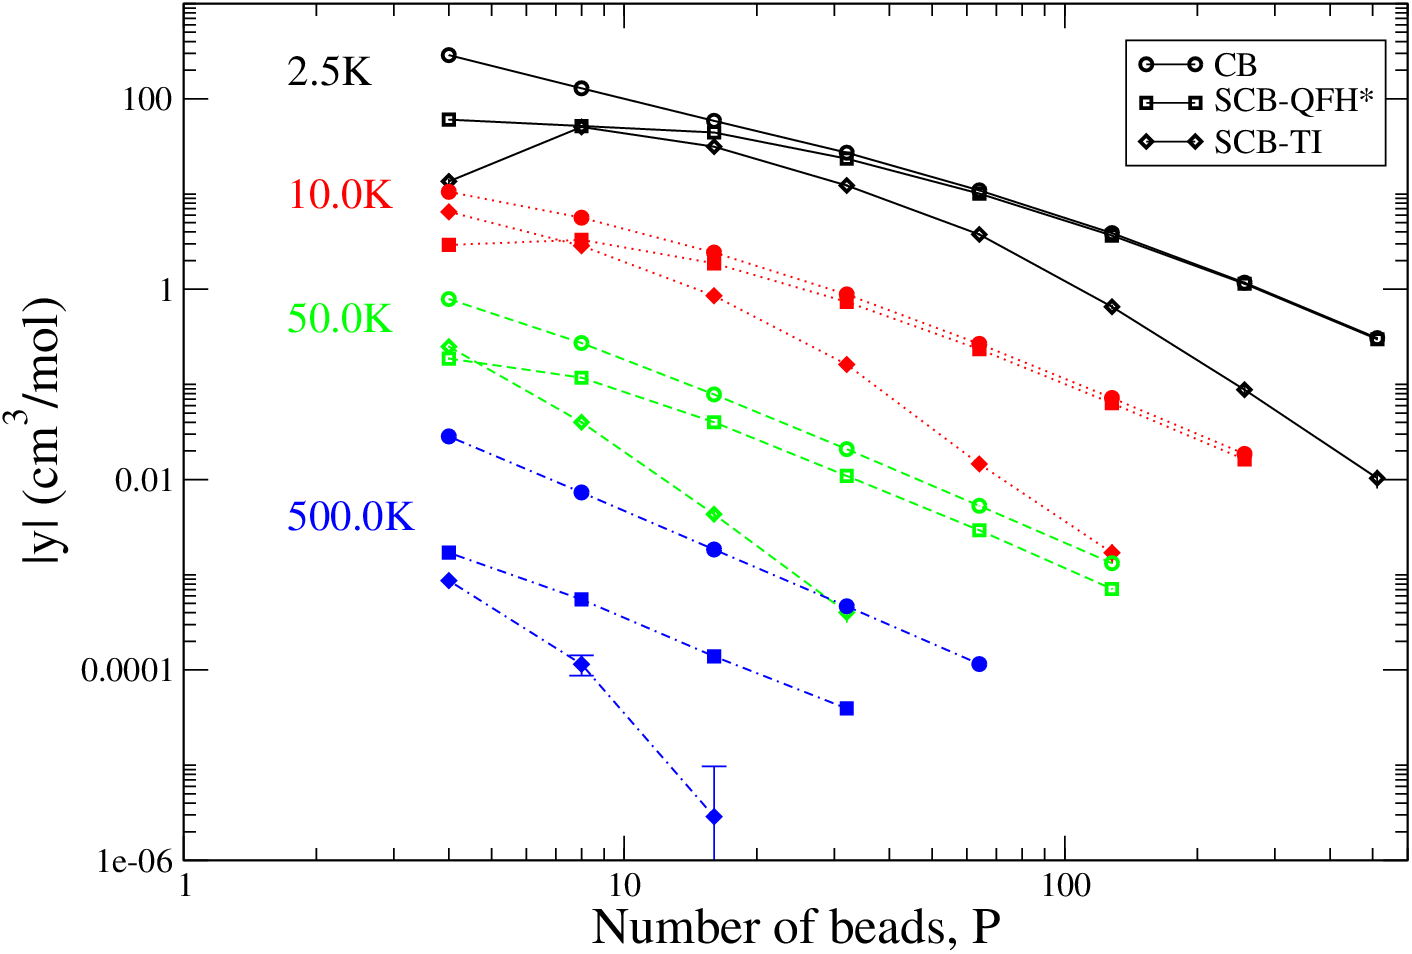
\includegraphics[scale=0.3,keepaspectratio]{Chapter-3/Figures/shMagVsP.png}
        \caption{Convergence factor, $y = [\Gamma(P,u) - \Gamma(P/2,u)]$ as a function of number of beads $P$. Symbols alternate filled or open with each temperature and indicate: classical-beads (CB) approach (circles); SCB-QFH* (squares); SCB-TI (diamonds). Temperatures are $T = 2.5~K$ (black open symbols connected by solid lines); $T = 10.0~K$ (red filled symbols connected by dotted lines); $T = 50.0~K$ (green open symbols connected by dashed lines); $T = 500.0~K$ (blue filled symbols connected by dash-dot lines). Confidence limits (68\%) are smaller than the symbol sizes except where shown.} \label{shMag}
    \end{figure}

    To assess the performance of SCB-QFH* and SCB-TI approaches against the CB approach in terms of achieving better precision, we plot the ratios of uncertainty of the quantity $y = [\Gamma(P,u) - \Gamma(P/2,u)]$, i.e. we plot $\sigma_y$(SCB-QFH*)/$\sigma_y$(CB) and $\sigma_y$(SCB-TI)/$\sigma_y$(CB) in Fig. \ref{uncRatios}. In order to make a fair comparison, we use the uncertainties due to the same number of MC steps ($1\times10^6$) for each case. In Fig. \ref{uncRatios} we observe that SCB-TI has a consistently lower uncertainty ratio than SCB-QFH*  for all $P$ except for $P$ = 4, where the $T$ = 2.5 and 5.0 K results for SCB-QFH* have slightly lower values. At these low temperatures, since $P > 4$ almost always, we do not worry too much about SCB-QFH* having lower uncertainty ratios because it does not affect the uncertainty of the overall result that much, and also because the values are only slightly lower. The ratio for SCB-QFH* is almost always greater than 1, suggesting that it is not expected to give better precision when compared to CB for most cases. For the cases where the SCB-QFH* ratio is less than 1, i.e. $T$ = 2.5 K and $P \le$ 128, we expect it to give better precision. The ratio for SCB-TI is almost always less than 1, suggesting that it is expected to give better precision when compared to CB for most cases. For the cases where the SCB-TI ratio is greater than 1, i.e. $T$ = 10.0 K and $P \le 8$, the magnitude is only marginally greater; as explained earlier, usually $P > 8$ is needed for accurate results when $T$ = 10.0 K.
    \begin{figure}
        \centering
        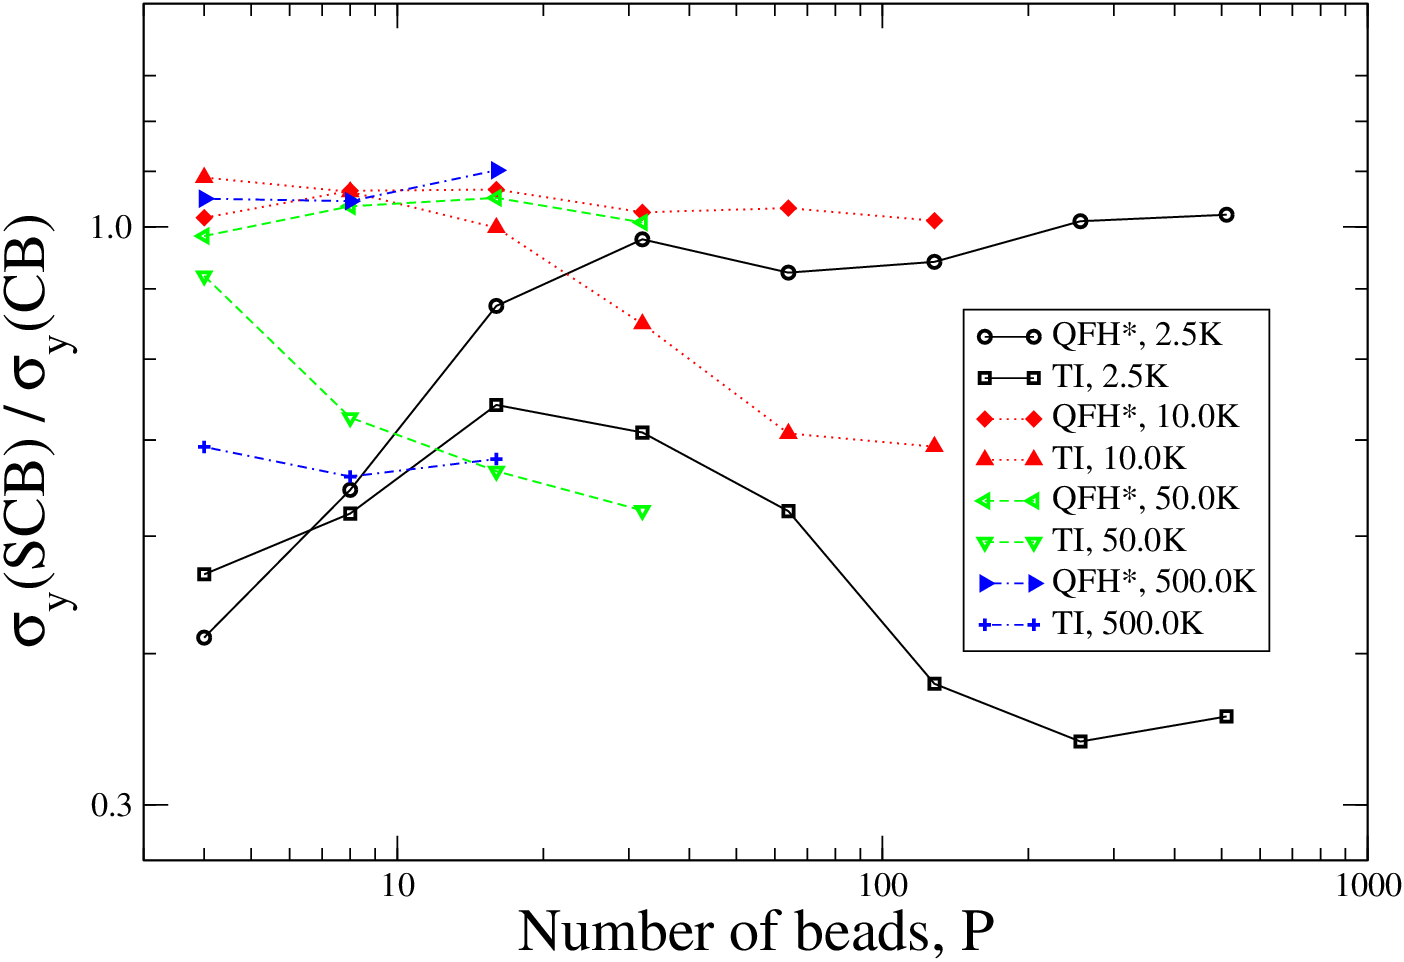
\includegraphics[scale=0.3,keepaspectratio]{Chapter-3/Figures/uncRatiosOct19.png}
        \caption{Uncertainty ratio of the convergence factor $\sigma_y(\rm{SCB})/\sigma_y (\rm{CB})$, where $y = [\Gamma(P,u) - \Gamma(P/2,u)]$, as a function of number of beads $P$.} \label{uncRatios}
    \end{figure}

    To assess the performance of SCB-QFH* and SCB-TI approaches against the CB approach in terms of the uncertainty achieved for a given period of time, in Fig. \ref{uncB21Hr}we plot the ratios of best-case uncertainties of the quantum second virial coefficient values, i.e., $\sigma B_2 (\text{SCB-QFH*})/\sigma B_2 (\text{CB})$ and $\sigma B_2 (\text{SCB-QFH*} )/\sigma B_2 (\text{CB})$ that would result if we used the best possible decompositions of each of the approaches and were only allowed a total simulation time of 1h per approach. Such an estimation of the best-case uncertainty for a total simulation time of 1 h is possible as a result of performing longer simulations of each of the fragments that form the decomposition (see Shaul et al. \cite{Shaul2012} for more details). We again observe that in Fig. \ref{uncB21Hr}, the SCB-TI approach has a lower uncertainty ratio than SCB-QFH* for all temperatures considered. Also, the ratio of SCB-TI is slightly less than 1 for most cases while that of SCB-QFH* is always greater than 1. This suggests that decomposition for the SCB-QFH* approach is expected to yield larger uncertainties for the quantum virial coefficient, compared to that of CB and SCB-TI approaches. The decomposition for the SCB-TI approach seems to be performing better than the SCB-QFH* approach, especially at lower temperatures, which is desirable because we normally tend to use large $P$ at these temperatures. Even in the cases where the SCB-TI ratio is greater than 1, it is only marginally greater and therefore it may be considered acceptable.
    \begin{figure}
        \centering
        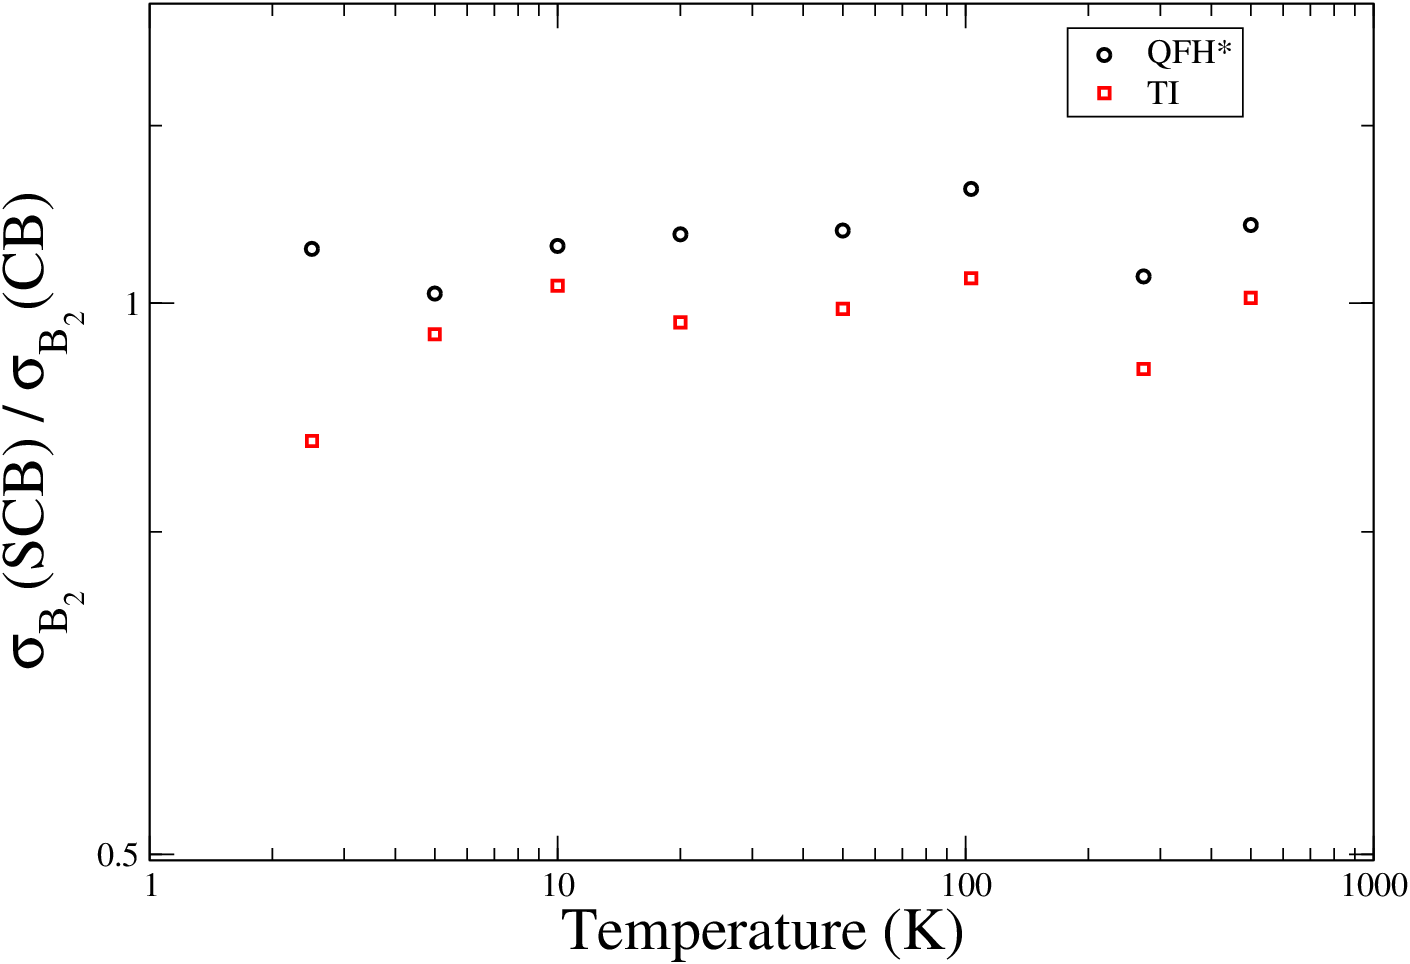
\includegraphics[scale=0.3,keepaspectratio]{Chapter-3/Figures/uncB21Hr.png}
        \caption{Uncertainty ratio $\sigma_{B_2}{\rm(SCB)}/\sigma_{B_2}{\rm{(CB)}}$ as a function of temperature, for a fixed total computation time of 1 CPU-hour.} \label{uncB21Hr}
    \end{figure}

    \section{Conclusions}
    \label{sec:heConclusion}
        We have implemented the PIMC method with two approaches based on semi-classical beads (SCB-QFH*,SCB-TI) and MSMC to compute more precise quantum virial coefficients for helium-4. The SCB results agree well with CB results as they are within statistical uncertainties of each other. The decomposition algorithm of Shaul et al.~\cite{Shaul2012} was implemented to achieve better efficiency of quantum virial coefficient calculations. We observed similar trends in decompositions of simulations in our SCB based approaches as was the case for the CB approach. For lower temperatures, the approximation $u^{\rm simple}$ to $u$ for finite $P$ is chosen as the preliminary approximation. As the temperature increases, the preliminary approximation preferred is the semi-classical approximation to $u^{\rm simple}$, and for high temperatures the semi-classical approximation to $u$ is preferred. Having chosen the preliminary approximation, the decomposition algorithm spends maximum time in the first step and the amount of time spent per step gradually decreases for subsequent steps. This is because the subsequent steps involve more computationally expensive calculations (either by shifting to $u$ from its semi-classical approximation, or by doubling $P$ from the previous step, or by shifting to the full potential $u$ from $u^{\rm simple}$) and by design, these steps also yield better and better precision. The decomposition algorithm was designed to allocate computational effort proportional to the difficulty of the computation, which is defined as (error~$\times$~uncertainty). The SCB-QFH* and SCB-TI approaches have comparable and better uncertainties respectively, for the steps that involve computing $[\Gamma(P,u) - \Gamma(P/2,u)]$ or $[\Gamma(P,u^{\rm simple}) - \Gamma(P/2,u^{\rm simple})]$. Since these steps involve significant computational costs and relatively low uncertainties, the amount of effort dedicated for them is lower, attenuating the effect of any efficiency brought to their calculation. As a result, the improvement of the precision of the resulting virial coefficient is only marginal. We note that if the decomposition algorithm is not being used, either because it is non-trivial to apply, or because virial coefficients are not being computed, the SCB-TI approach performs much better than both SCB-QFH* and CB approaches, which is what we would expect anyway from the use of a higher order propagator.

        In summary, we found the following order for the rate of convergence with respect to number of beads $P$: SCB-TI $>$ SCB-QFH* $>$ CB. We expect a similar trend for the rate of convergence with respect to $P$ for higher order coefficients as well, because of the use of the higher order TI propagator. The order for precision was found to be: SCB-TI $>$ SCB-QFH*. Compared to CB, QFH* is always worse but only marginally so; TI is almost always better and only marginally worse for a few temperatures. We expected a trend similar to the rate of convergence with $P$ for the precision as well, even for $B_2$ calculations. Since this was not what we observed, partially due to the decomposition algorithm, an understanding of the order of precision for higher order coefficients for the SCB based approaches compared to CB approach would require further investigation. However, we do expect the order between SCB based approaches to remain the same, i.e., SCB-TI $>$ SCB-QFH*.

\chapter{Hydrogen}
    \section{Motivation}
        Hydrogen is an extremely important ingredient in many industries including fertilizers, petroleum, aerospace as rocket fuel and energy as an alternative fuel source \cite{Jacobsen2007}. Additionally, the properties of mixtures of hydrogen and other gases are also important in several other fields ranging from metrology (H$_{\rm 2}$ + H$_{\rm 2}$O) \cite{Hodges2004} to astrophysics (H$_{\rm 2}$ + He) \cite{Boothroyd2002,Boothroyd2003} to superfluidics \cite{Patkowski2008,Grebenev2000}. Therefore, computing really precise and accurate physical properties of hydrgoen is vital to several industries as well as research institutions.

        Historically, hydrogen has been, and still is, one of the most studied compounds in quantum chemistry owing to its extemely simple electronic structure comprising of just one electron. Molecular hydrogen exists in two forms with significantly different physical properties \cite{Jacobsen2007}: 1) parahydrogen with anti-parallel nuclear spins and 2) orthohydrogen with parallel nuclear spins. Hydrogen also has two isotopes Deuterium (D) and Tritium (T) with 1 and 2 neutrons respectively. Several studies \cite{Goodwin1963,Kolos1986,Schwenke1988,Mielke2002,Manzhos2010,Garberoglio2010,Garberoglio2012,Sakoda2012,Garberoglio2013,Garberoglio2014} (both computational as well as experimental) of different combinations of the hydrogen molecule and its isotopes ($\allowbreak {\rm H_2, H_3, (H_2)_2, (H_2)_3, HD, HT, D_2, T_2}$ etc.) have been performed to gain further insight into the nature of interactions of these systems. However, for the purpose of evaluating fully quantum virial coefficients using \abinitio{} potentials, we restrict our attention primarily to the hydrogen dimer ${\rm (H_2)_2}$ and consider both the rigid as well as flexible monomer cases.

    \section{Recent Developments}
        In this section, we give an overview of some the \abinitio{} \PESs{} that have been developed for studing the hydrogen dimer and in the interest of brevity, we restrict our discussion to the \PESs{} that were developed on or after the year 2000.\\
 
        Diep and Johnson's \cite{Diep2000} pioneering work lead not only to the development of the PIMC method but also two \abinitio{} \PESs{} for the dimer with rigid monomers. One using the vibrationally-averaged bond length of the dimer and anohter using a slightly smaller equilibrium value, in order to study the effect of bond lengths on the \PESs{}. 37 unique angular configurations were used in the constuction of these \PESs{} (and their corresponding spherical harmonics fits) and electron correlation effects were accounted at the MP2, MP3, MP4 and CCDS(T) levels of theory. They observed excellent agreement of their calculated second virial coefficient values with experiments for T = 15 to 500K. They also concluded that the differences observed in the \PESs{} based on different bond lengths were small. Boothroyd et al. \cite{Boothroyd2002} reported a rigid monomer PES (Ad) that was fit to \Sim{} 48 000 \abinitio{} energies out of which \Sim{} 42 000 were computed using the MRD-CI program of Buenker and Peyerimhoff \hl{include other papers as well} \cite{Buenker1974}. They observed significant improvement over previous \PESs{} in terms of its rms error. Robert J. Hinde \cite{Hinde2008} reported a six dimensional PES that included monomer flexibility as well and used it for studying the IR and Raman transition energies. Patkowski et al. \cite{Patkowski2008} reported a rigid monomer PES that was computed at the CCSD(T) level of theory using very large orbital basis sets. They reported second virial coefficients that were in better agreement with experiments than previous \PESs{}. It was also found that including quantum effects becomes important at \Sim{} 200K for PIMC calculations of virial coefficients. Most recently, Van and Deiters \cite{Tat2015} have reported a new \abinitio{} PES at the CCSD(T) level of theory and observed very good agreement of their calculated virial coefficients with experiemental results (where available). 
    \section{Computational details}
        We performed calculations for three different models of H$_2$, differing primarily in their treatment of the intramolecular bond:

        Model 1 ($s_1$): We use the rigid inter-molecular potential due to Patkowski et al.\cite{Patkowski2008} (denoted as V$_{pat}$), with the H-H bond length fixed at all temperatures to the ground state value $r_0 (= $1.448736 Bohr, same as in \cite{Patkowski2008}). Due to nonphysical energies returned by V$_{pat}$ at small inter-molecular separations, an artificial spherical hard core (with a diameter $d = 1${\AA}) is used.

        Model 2 ($s_2$): We use the flexible inter-molecular potential due to Garberoglio et al.\cite{Garberoglio2012} (denoted as V$_{hp}$), with a fixed but temperature-dependent H-H bond length, computed at each temperature to its average value $\left< r \right>_T$ (see Sec. \ref{sec:novel algorithms} for details). For V$_{hp}$, instead of an artificial spherical hard core, the potential is calculated with an inter-molecular distance $R$ which is the larger of ($R,\: 1.4${\AA}) and a bond length $b$ which is the smaller of ($b,\: 1.2${\AA}).

        Model 3 ($s_3$): We use V$_{hp}$ and allow the bond length value to vary during the calculation. The intra-molecular potential that we use is due to Mielke et al.\cite{Mielke2002} who fitted the data of Kolos et al.\cite{Kolos1986} to obtain a ground state potential.

        Mayer sampling Monte Carlo was used to sample the intermolecular distance, while the direct methods described above were used to sample path-integral image position, orientations and (where appropriate) bond lengths. It should be noted that these different MC moves were chosen with equal probability within each simulation. We ran simulations at 33 temperatures going from $T =$ 15 K $\to$ 2000 K to compare our $s_1, s_2$ and $s_3$ results against Garberoglio et al.\cite{Garberoglio2014}. We ran additional simulations at 53 temperatures going from $T =$ 16 K $\to$ 423.15 K for which experimental $B_2$ values were reported in Goodwin et al.\cite{Goodwin1963}. Although the $B_2$ values in \cite{Garberoglio2014} were calculated after choosing $P$ as a function of $T$, we ran calculations for $P = 8, 16, 32$ and $64$ for all temperatures considered because we wanted to assess the performance of the algorithms. For each value of $P$, we used a total of $10^7$ samples to evaluate the virial coefficient using the MSMC\cite{Singh2004} method. We divide the $10^7$ samples into $10^4$ blocks of $10^3$ samples each and compute block averages for the different quantities prescribed by MSMC. Using the $10^4$ block-averages, we calculate the overall averages and their standard error, and use error propagation formulas to arrive at the final uncertainties (reported here) of the virial coefficients. A reference hard sphere diameter of 3{\AA} was used for all simulations.
        Note that all simulations performed for the conditions mentioned above, were to compute the Boltzmann contribution to the virial coefficient using only Boltzmann-type configuration samples. Additionally, we also performed simulations, for each of the cases mentioned above, to compute the exchange contribution to the virial coefficient using only exchange-type configuration samples. We combine the two contributions according to their ratio as given in Fig. 2 of Garberoglio et al. \cite{Garberoglio2014} to compute the final virial coefficient values reported here. Since the ratio was zero for $T > 225$K, suggesting that exchange contributions were negligible at higher temperatures, we evaluated the exchange contributions only for temperatures $T \le 225 K$. Since the values of ratios we used were basically read off their graph and then fitted to different temperatures, there is a certain amount of random human error, for $T \le 225 K$, in the final virial coefficient results, for all Models. 
    \section{Results and discussion}
        Presented below are the results of our virial coefficient calculations as a function of temperature. Since H$_2$ was considered as a test case, we tried to reproduce previous results of Garberoglio et al.\cite{Garberoglio2014} who reported second virial coefficients using VEGAS\cite{Lepage1972} algorithm for models $s_1, s_2$ and $s_3$. Hence, we just compare our values with theirs(for \emph{para}-H$_2$) as a reference for the sake of simplicity (for other literature values and/or experimental data, the interested reader may see references\cite{Goodwin1963, Patkowski2008, Leachman2009, Sakoda2012, Garberoglio2012, Garberoglio2014}). Henceforth, by ``reference values", we mean the values reported in \cite{Garberoglio2014} under similar conditions.

        We have also evaluated the performance in terms of percentage of moves accepted for both the orientation and the bond length algorithms. We have shown the same as a function of temperature for the different simulation options mentioned above.

        \subsection{Rigid-bond models -- Orientation trials}
            In this section we examine the results for Models 1 and 2, which are the rigid-bond models, by which we scrutinize the validity and performance of the orientation-sampling trial, by itself. We begin by noting that the number of images used by Garberoglio for achieving converged results \cite{Patkowski2008} for Model 1 was calculated as:
            \begin{equation}
            \label{eq:s1P}
                P = 3600 K/T
            \end{equation}
            
            According to Eq. \eqref{eq:s1P} the temperature at which we require $P > 64$ to achieve converged results for Model 1 is 50 K. We also note that we have used a maximum of $P = 64$ images for all temperatures. Therefore we expect to see significant differences between our virial coefficient values for Model 1 and the corresponding reference values for $T \le 50 K$.
            
            Similarly, we have for Model 2 \cite{Garberoglio2012}:
            \begin{equation}
            \label{eq:s2P}
                P = \lceil 2500 K/T + 7 \rceil
            \end{equation}
            where $\lceil x \rceil$ denotes the smallest integer larger than $x$.
            
            According to Eq. \eqref{eq:s2P} the temperature at which we require $P > 64$ to achieve converged results for Model 2 is 40 K. Therefore we expect to see significant differences between our virial coefficient values for Model 2 and the corresponding reference values for $T \le 40 K$. Although for a given temperature $T$, Eqs. \eqref{eq:s1P} and \eqref{eq:s2P} provide a good estimate of $P$ required for achieving converged results, in practice, one might be able to achieve convergence with fewer $P$ as well.

            \subsubsection{$B_2$ values}
                \begin{figure}[!htbp]
                    \centering
                    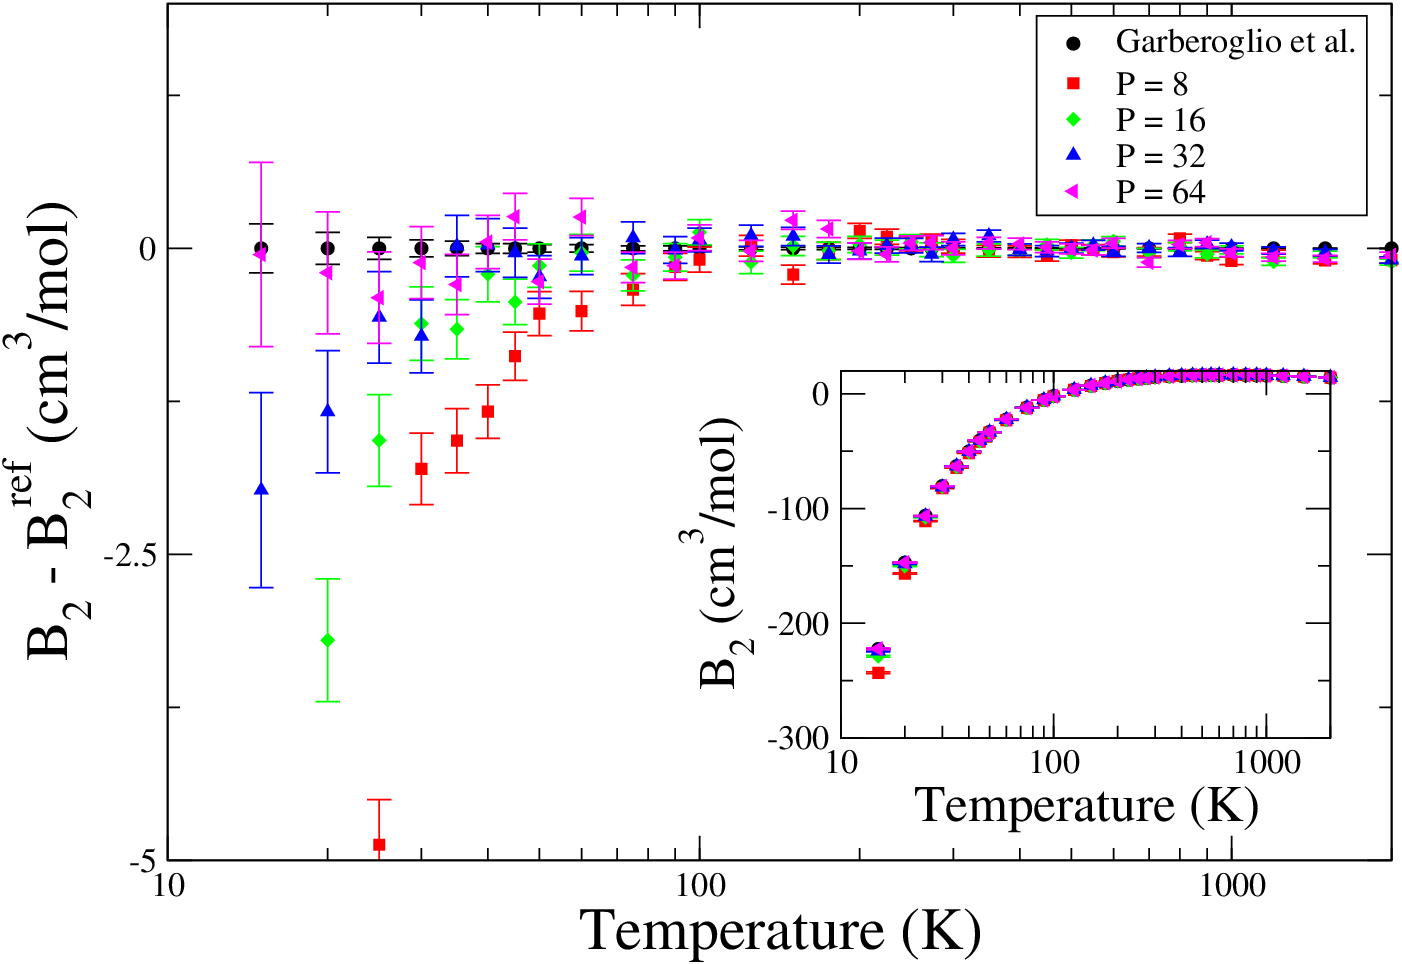
\includegraphics[width=10cm,keepaspectratio]{Chapter-4/Figures/s1GarberoglioAll.png}
                    \caption{Fully quantum second virial coefficient ($B_2$) values compared against reference values \cite{Garberoglio2014}, for Model 1. Main figure is the difference between the values computed here and the reference values, while the inset shows the coefficients before differencing. The value of the number of path-integral beads is $P$, and the results for different $P$ are as indicated in the legend. Error bars are drawn at $\mu \pm \sigma$ where $\mu$ is the mean value and $\sigma$ is the standard error. It should be noted however, that the 95\% confidence interval is given by $\mu \pm 2\sigma$.}
                    \label{fig:r0}
                \end{figure}
                In Fig. \ref{fig:r0} we show our $B_2$ values and the reference values for Model 1 as a function of temperature. It can be seen that the agreement between reference values and our results is generally good over the wide range of temperatures considered (15 K to 2000 K). The agreement is particularly good for $T > 50 K$ where our results using $P = 64$ images are sufficient enough to achieve convergence according to Eq. \eqref{eq:s1P}. For $T \le 50 K$, we observe statistically significant disagreement between our results (for all $P$ considered) and reference values and the magnitude of this deviation decreases with increasing $P$ and/or $T$ and vice-versa. As explained earlier, this behavior is expected because the number of images we use is not sufficient for convergence according to Eq. \eqref{eq:s1P}. It should be noted that in Fig. \ref{fig:r0} the range of the $y$-axis was chosen to highlight the differences over the whole range of temperatures considered and as a result we did not include some data points (whose $B_2$ value was lesser than -5 cm$^3$/mol), especially for low temperatures. However, these data points are for lower-$P$ cases where the virial coefficient values have not yet converged and so we could afford to exclude them from the graphs.
                
                \begin{figure}[!htbp]
                    \centering
                    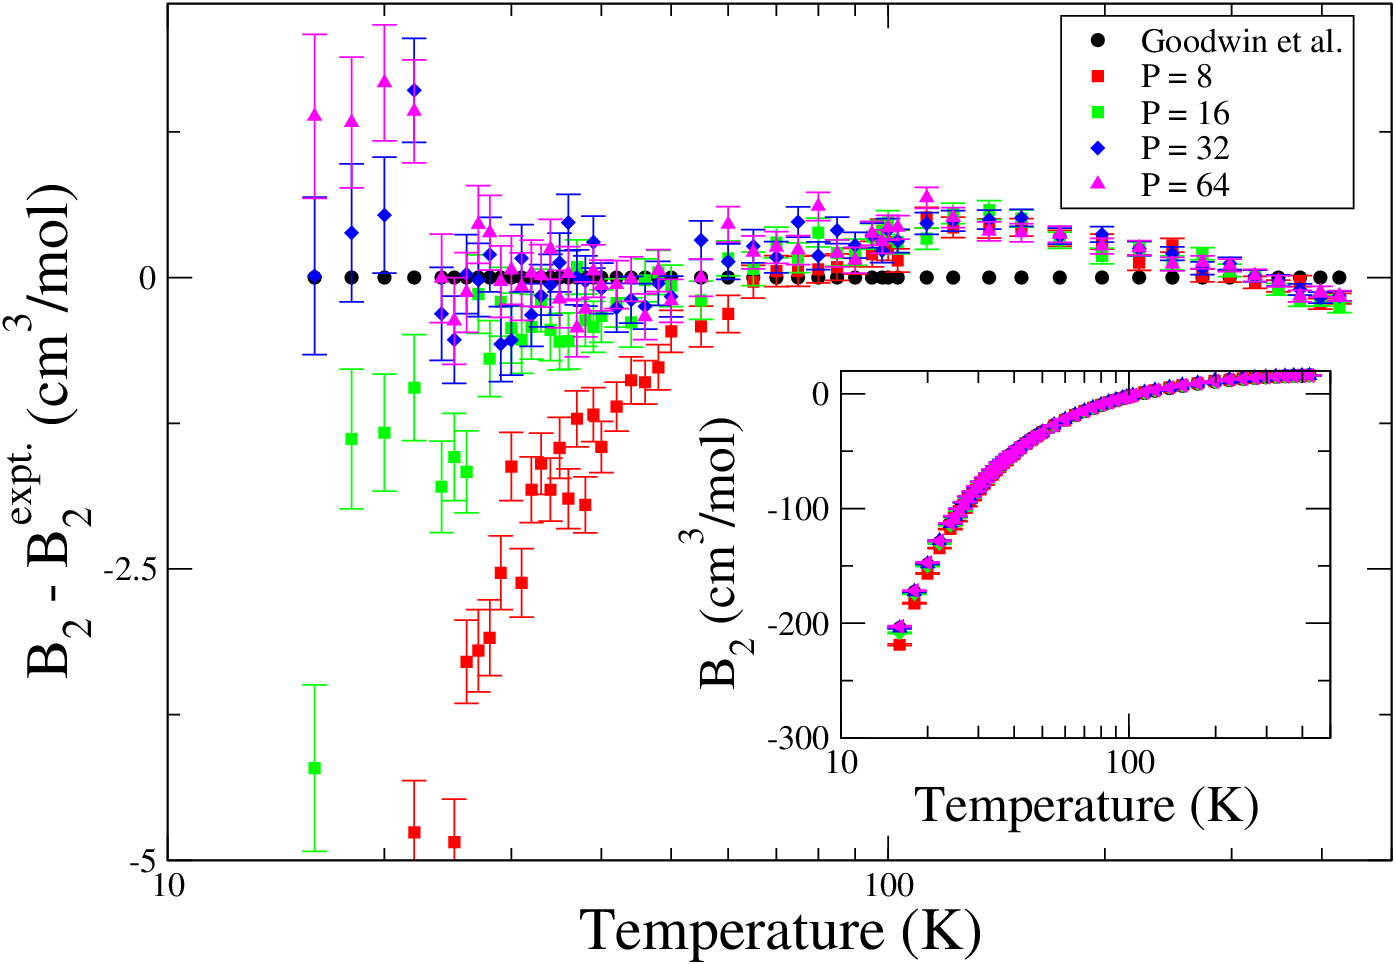
\includegraphics[scale=0.20,keepaspectratio]{Chapter-4/Figures/s1GoodwinAll.png}
                    \caption{Same as Fig. \ref{fig:r0}, but with comparison made to experimental data of Goodwin et al.\cite{Goodwin1963} rather than computed values from \cite{Garberoglio2014}.}
                    \label{fig:r0Goodwin}
                \end{figure}
                In Fig. \ref{fig:r0Goodwin} we compare our $B_2$ values for Model 1 against experimental results of Goodwin et al.\cite{Goodwin1963}. We observe particularly good agreement in two ranges of temperatures, $24 K \le T \le 50 K$ and $ 248.15 K \le T \le 423.15 K$, and significant deviations for other temperatures. Since we expect our results to have not converged for $T \le 50 K$, we consider the agreement in the range $24 K \le T \le 50 K$ to be fortuitous. At the higher temperature range where our results are converged according to Eq. \eqref{eq:s1P}, the agreement is of course expected. One possible reason for the disagreement observed at higher temperatures could be due to poor quality of the function fitted to experimental data at these temperatures. The disagreement observed at lower temperatures can be attributed to calculations involving insufficient $P$. It should be noted that in Fig. \ref{fig:r0Goodwin} the range of the $y$-axis was chosen to highlight the differences over the whole range of temperatures considered and as a result we did not include some data points (whose $B_2$ value was lesser than -5 cm$^3$/mol), especially for low temperatures. However, these data points are for lower-$P$ cases where the virial coefficient values have not yet converged and so we could afford to exclude them from the graphs.

                \begin{figure}[!htbp]
                    \centering
                    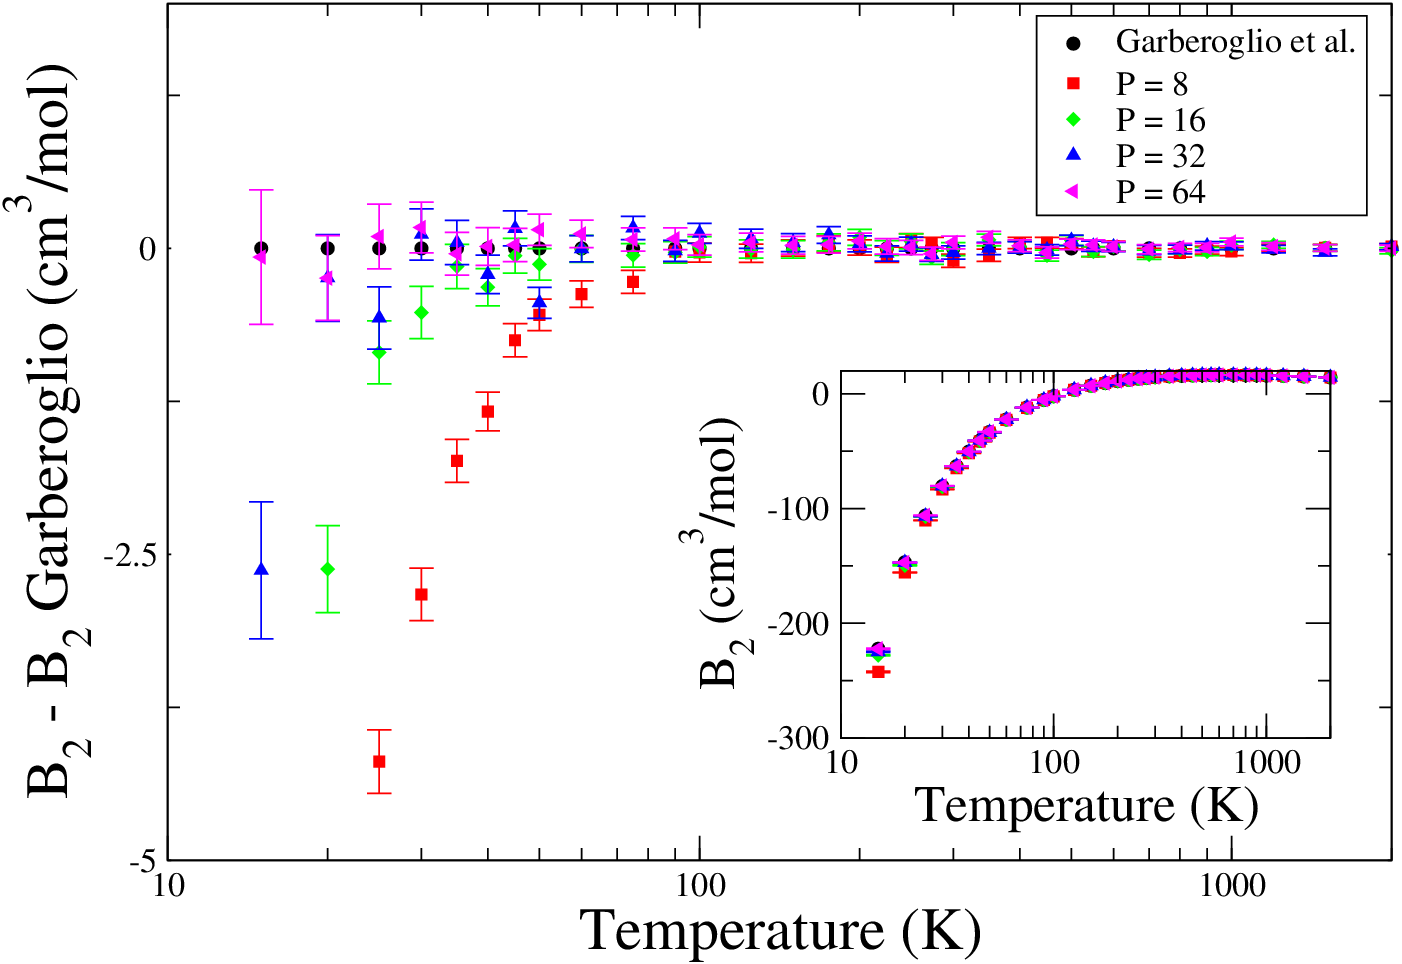
\includegraphics[scale=0.20,keepaspectratio]{Chapter-4/Figures/s2GarberoglioAll.png}
                    \caption{Same as Fig. \ref{fig:r0}, but values shown are those computed for Model 2 rather than Model 1.}
                    \label{fig:rT}
                \end{figure}
                In Fig. \ref{fig:rT} we show our $B_2$ values and the reference values for Model 2 as a function of temperature. It can be seen that the agreement between reference values and our results is particularly good for all temperatures except $T = 15 K$ and $25 K$ where our results have not converged (in accordance with Eq. \eqref{eq:s2P}). For a few temperatures below 40 K, we point out that our results have converged using fewer $P$ than that prescribed by Eq. \eqref{eq:s2P}. It should be noted that in Fig. \ref{fig:rT} the range of the $y$-axis was chosen to highlight the differences over the whole range of temperatures considered and as a result we did not include some data points (whose $B_2$ value was lesser than -5 cm$^3$/mol), especially for low temperatures. However, these data points are for lower-$P$ cases where the virial coefficient values have not yet converged and so we could afford to exclude them from the graphs.

            \subsubsection{Orientation algorithm performance}
                \label{sec:orPerformance}
                \begin{figure}[!htbp]
                    \centering
                    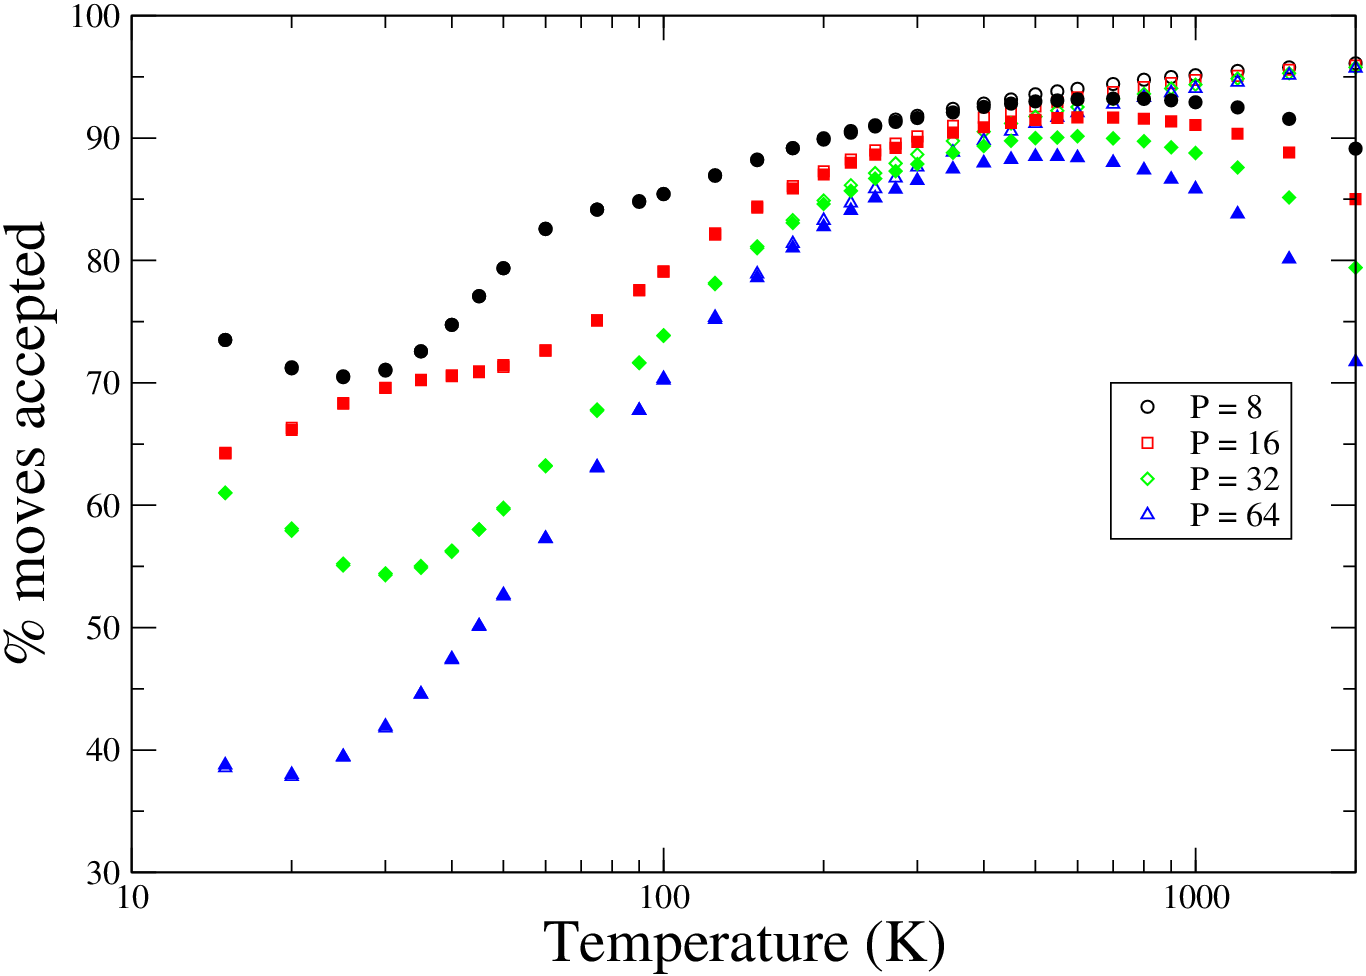
\includegraphics[scale=0.20,keepaspectratio]{Chapter-4/Figures/s12orAcc.png}
                    \caption{Performance of the orientation move for simulation options $s_1$ and $s_2$. Values for $s_1$ are represented using open symbols while that for $s_2$ are represented using filled symbols with the same shape.}
                    \label{fig:r0Acc}
                \end{figure}

                In fig. \ref{fig:r0Acc} we show the percentage of orientation moves that were accepted as a function of temperature for simulation options $s_1$ and $s_2$. Although we require more $P$ to accurately capture the nuclear quantum effects at low temperature, the efficiency of the algorithm decreases with increasing $P$ as is evident in the figure. As explained earlier, this is because we achieve exact sampling of the angle $\alpha$ only for the $P/2$ images that are placed in the last step of the orientation algorithm. For the other $P/2$ images, the sampling is approximate and not exact. Still, the acceptance rate at all conditions is quite good, and in the worst case hovers around 40\%, which means that roughly two attempts at generating a configuration are required to produce one that is acceptable. Given that the new configuration is completely uncorrelated from the one preceding it, this represents a significant improvement in the efficiency of sampling of the path-integral conformations.

                It is worth noting that in fig. \ref{fig:r0Acc}, there is a significant change in the behavior of the curves for $s_1$ and $s_2$, only for temperatures $\ge$ 700 K, where the performance for the $s_1$ case is increasing while that of $s_2$ is decreasing. To explain this phenomena and gain further insight into the nature of the difference between the actual distribution $\pi({\mathbf b})$ (Eq. \eqref{eq:piTotal}) and the approximate distribution $\tilde\pi({\mathbf b})$ (Eq. \eqref{eq:piTilde}), we ran simulations for a few hypothetical conditions and collected histograms of the angle between image 0 and image $P'$. We generated configurations by setting $P' = $ 2 and $k_h = $ 0.5 \AA$^{-2}$, and adjusting the simulation temperature accordingly (to hypothetical values). After choosing uniformly random orientations for all images as part of a MC trial, we accept or reject the trail based on $\pi ({\mathbf b})$ (Eq. \eqref{eq:piTotal}). We noted in Sec. \ref{subsec:orMove} that the ratio of the actual and approximate distribution for any image $j$ would be farthest from 1 for the first step of the algorithm. Therefore the histogram farthest away from $\pi ({\mathbf b})$, for the angle between the same set of images can be evaluated analytically using the approximate distribution function and assuming image $P'$ was placed in the first step (i.e., using Eq. \eqref{eq:piTildebj} with $j = P'$ and $\psi = 0$). By comparing these two histograms, we were able to visualize the nature of difference between the two distributions qualitatively. We repeated the above exercise for $P' =$ 4, 8 and $k_h =$ 5 \AA$^{-2}$, 50 \AA$^{-2}$ and their different permutations as well. It should be noted that all histograms were collected using 100 bins and 10$^8$ samples each.

                \begin{figure}[!htbp]
                    \centering
                    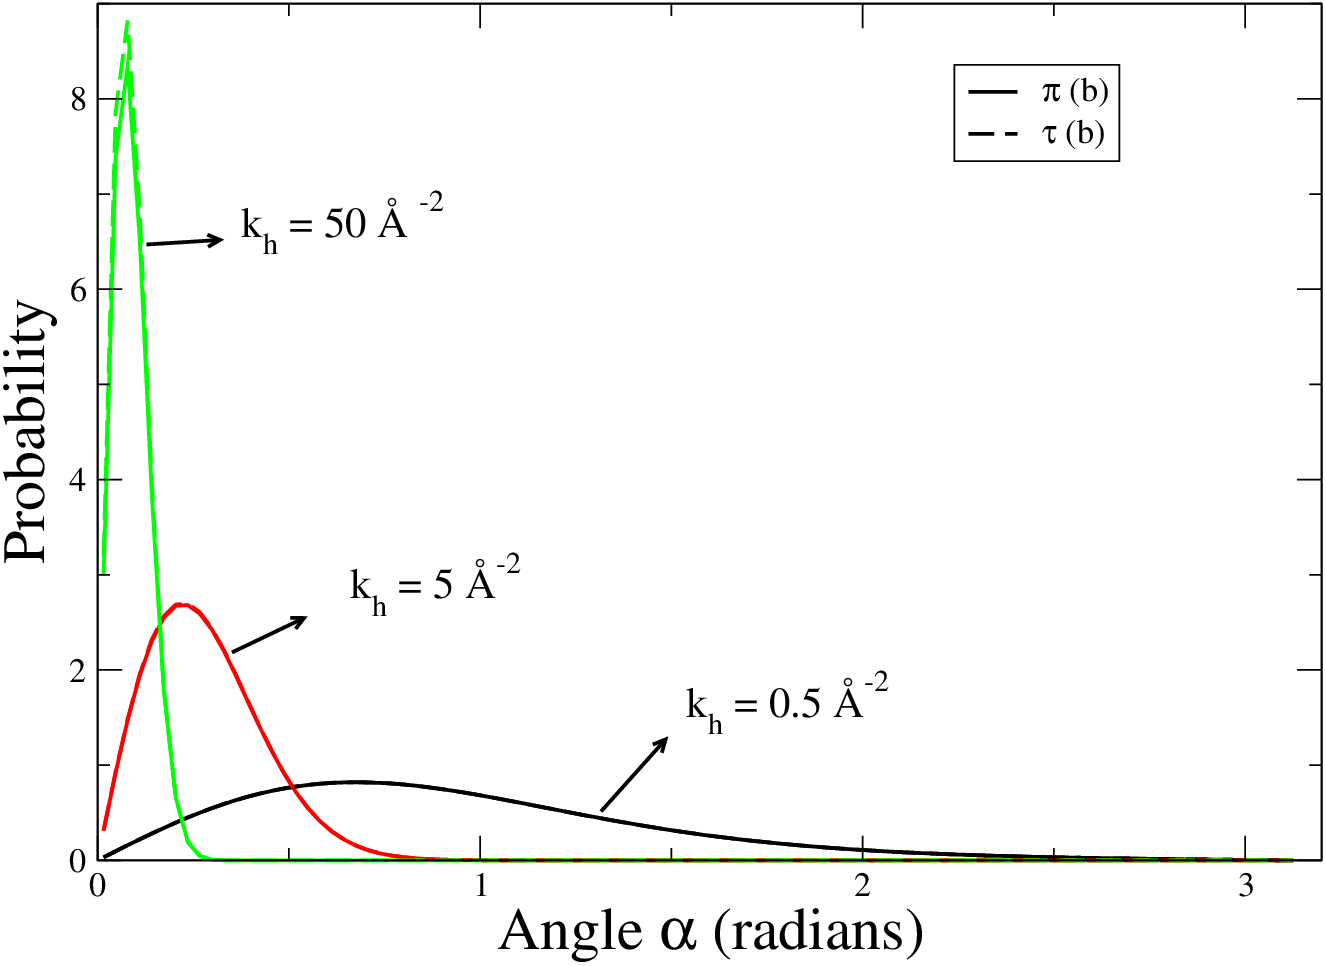
\includegraphics[scale=0.20,keepaspectratio]{Chapter-4/Figures/phi2B.png}
                    \caption{Approximate and actual probability distributions for $P' =$ 2.}
                    \label{fig:phi2B}
                \end{figure}

                \begin{figure}[!htbp]
                    \centering
                    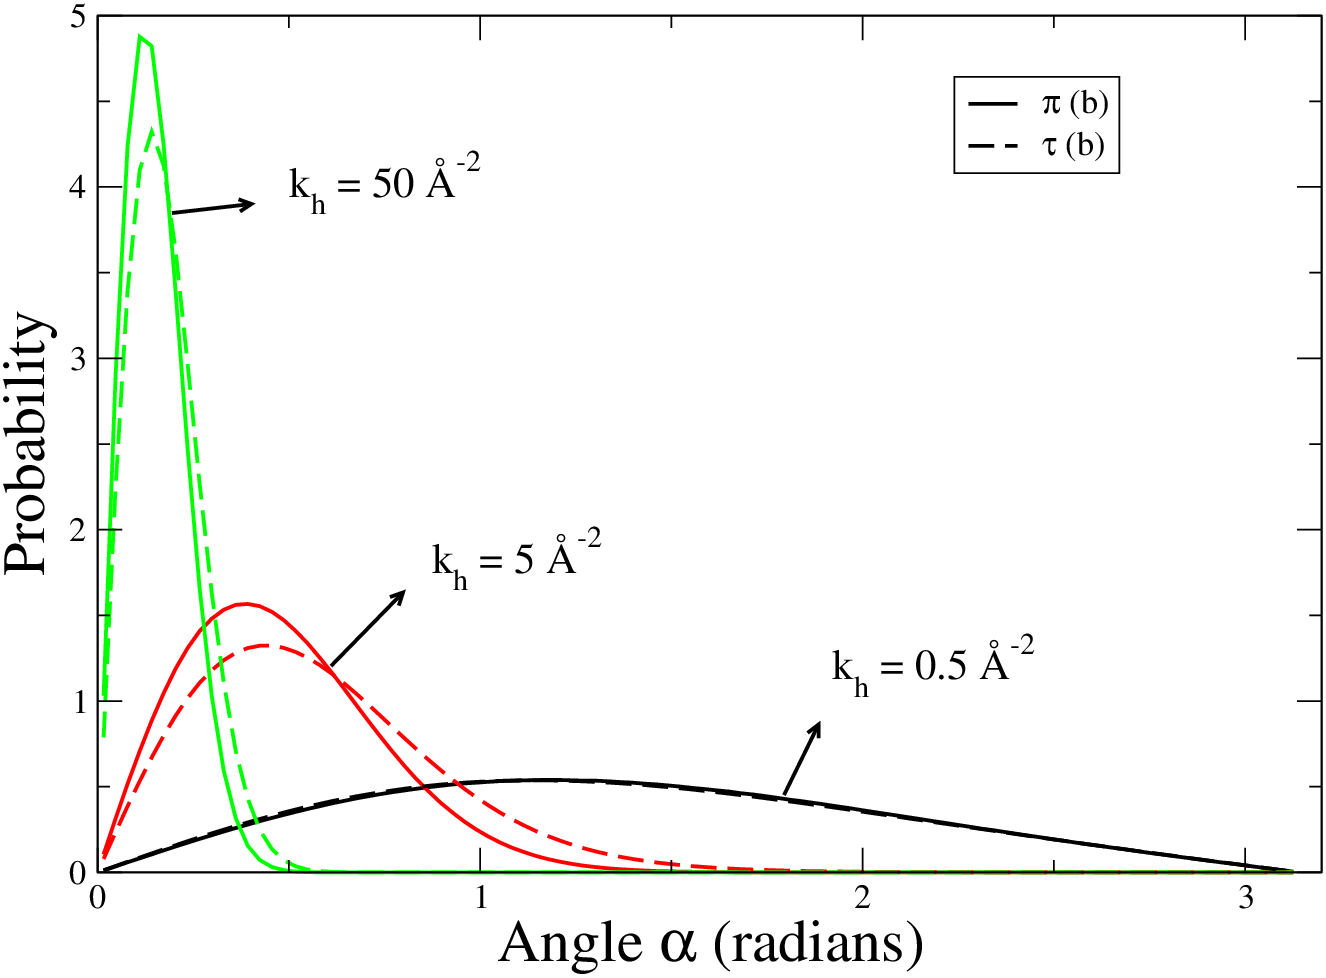
\includegraphics[scale=0.20,keepaspectratio]{Chapter-4/Figures/phi4B.png}
                    \caption{Approximate and actual probability distributions for $P' =$ 4.}
                    \label{fig:phi4B}
                \end{figure}

                \begin{figure}[!htbp]
                    \centering
                    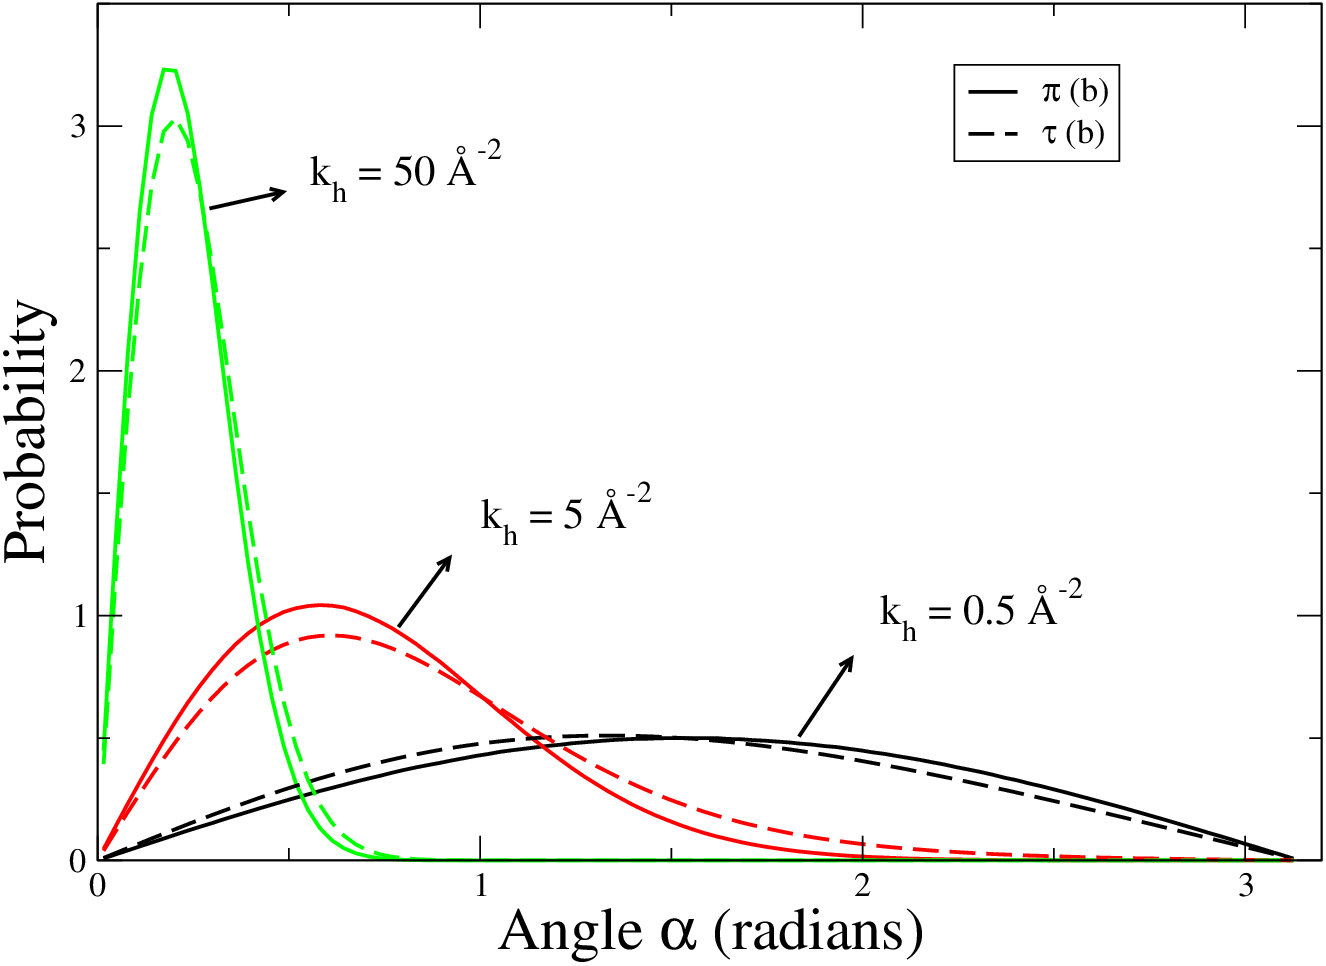
\includegraphics[scale=0.20,keepaspectratio]{Chapter-4/Figures/phi8B.png}
                    \caption{Approximate and actual probability distributions for $P' =$ 8.}
                    \label{fig:phi8B}
                \end{figure}

                From figs. \ref{fig:phi2B}, \ref{fig:phi4B} and \ref{fig:phi8B}, we can infer the following:
                \begin{itemize}
                    \item For a given $P$, we observe that the approximate distribution seems to be under-predicting for some range of angles and over-predicting for other ranges, as it must for both distributions to be normalized.
                    \item For a given $P$, the actual distribution gets narrower and taller as we increase $k_h$. This is to be expected because springs with high $k_h$ values tend to prefer smaller angles $\alpha$ as they are harmonically more favorable. The generally increasing trend in the percentage moves accepted as a function of temperature (as seen in fig. \ref{fig:r0Acc}) can be explained due to this phenomenon.
                \end{itemize}

                To further elucidate the difference between the approximate and actual distributions, we plot the ratio of the actual and the approximate distributions on the $y$-axis and the approximate distribution on the $x$-axis for the different hypothetical conditions mentioned above. For ease of explanation, we define ``closeness" between the two distributions as the deviation of $y$-coordinate from the $y =$ 1-line in figs. \ref{fig:ratio2B}, \ref{fig:ratio4B} and \ref{fig:ratio8B}.

                \begin{figure}[!htbp]
                    \centering
                    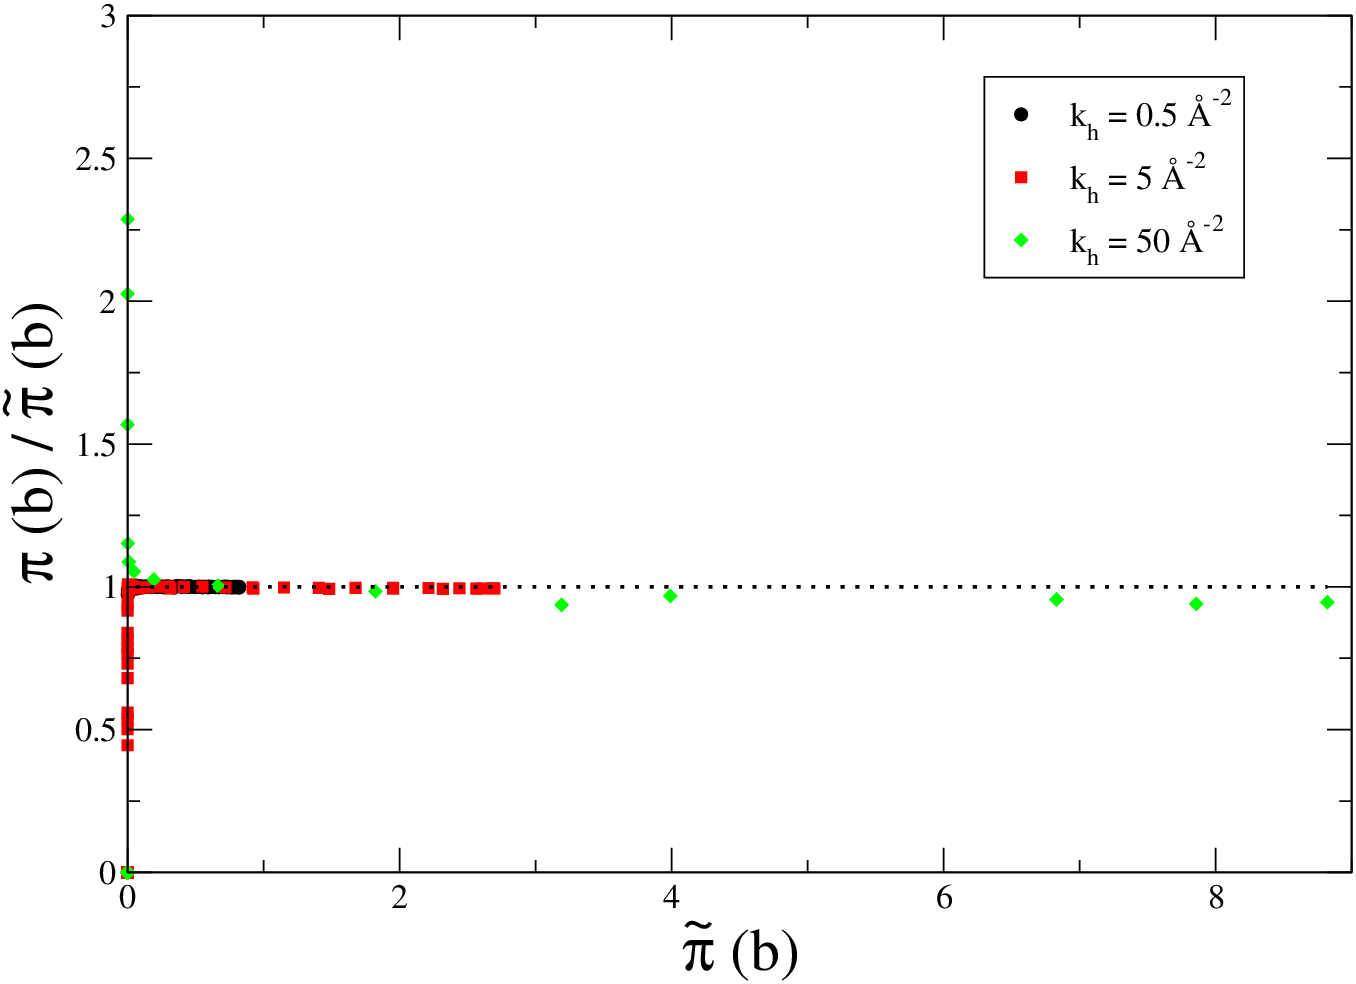
\includegraphics[scale=0.20,keepaspectratio]{Chapter-4/Figures/ratio2B.png}
                    \caption{Ratio of the approximate and actual probability distributions for $P' =$ 2.}
                    \label{fig:ratio2B}
                \end{figure}

                \begin{figure}[!htbp]
                    \centering
                    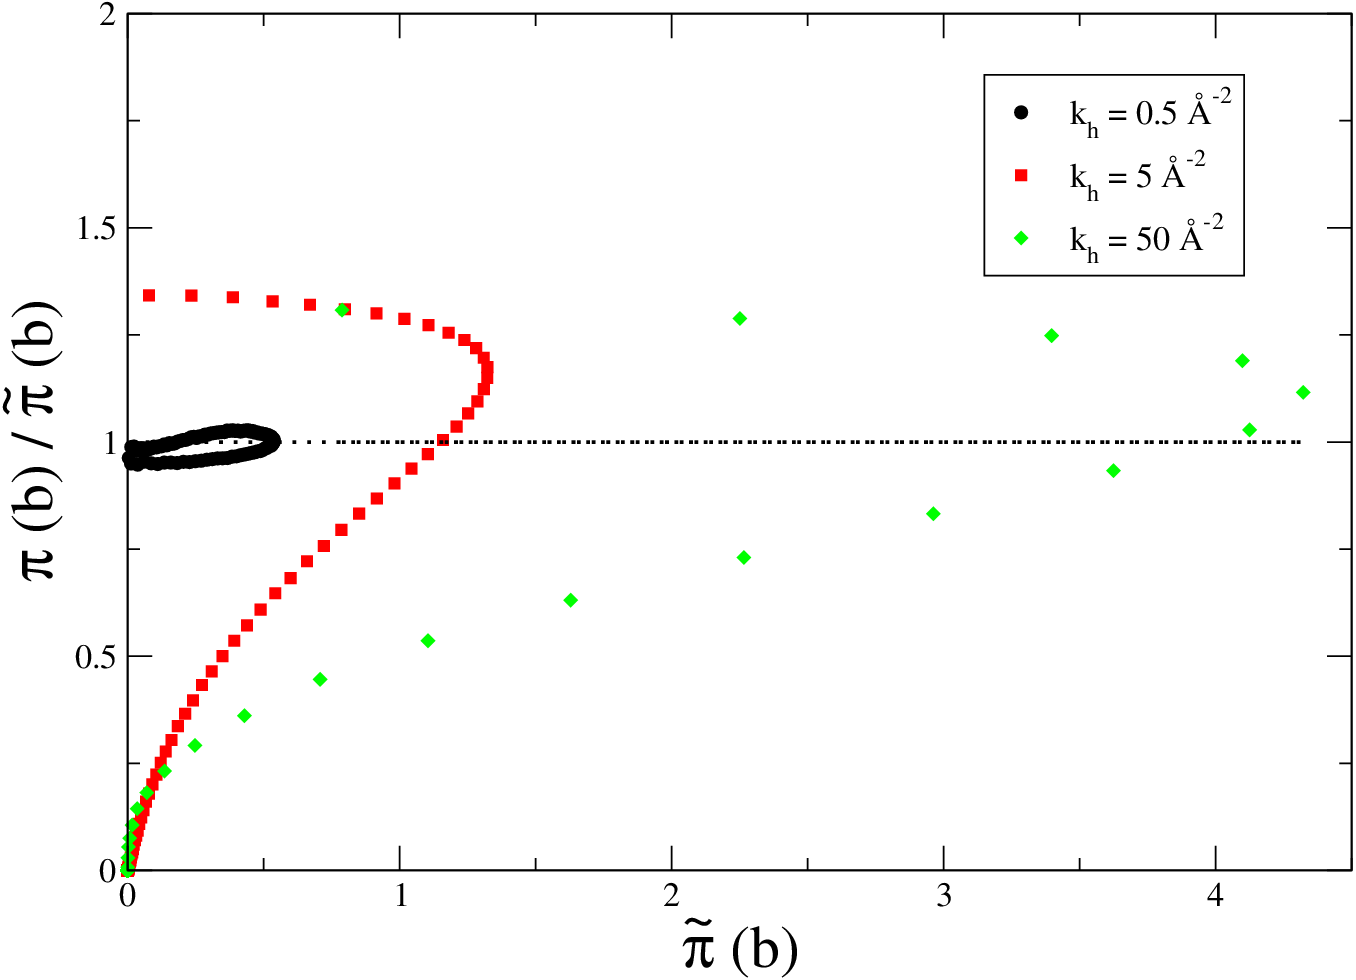
\includegraphics[scale=0.20,keepaspectratio]{Chapter-4/Figures/ratio4B.png}
                    \caption{Ratio of the approximate and actual probability distributions for $P' =$ 4.}
                    \label{fig:ratio4B}
                \end{figure}

                \begin{figure}[!htbp]
                    \centering
                    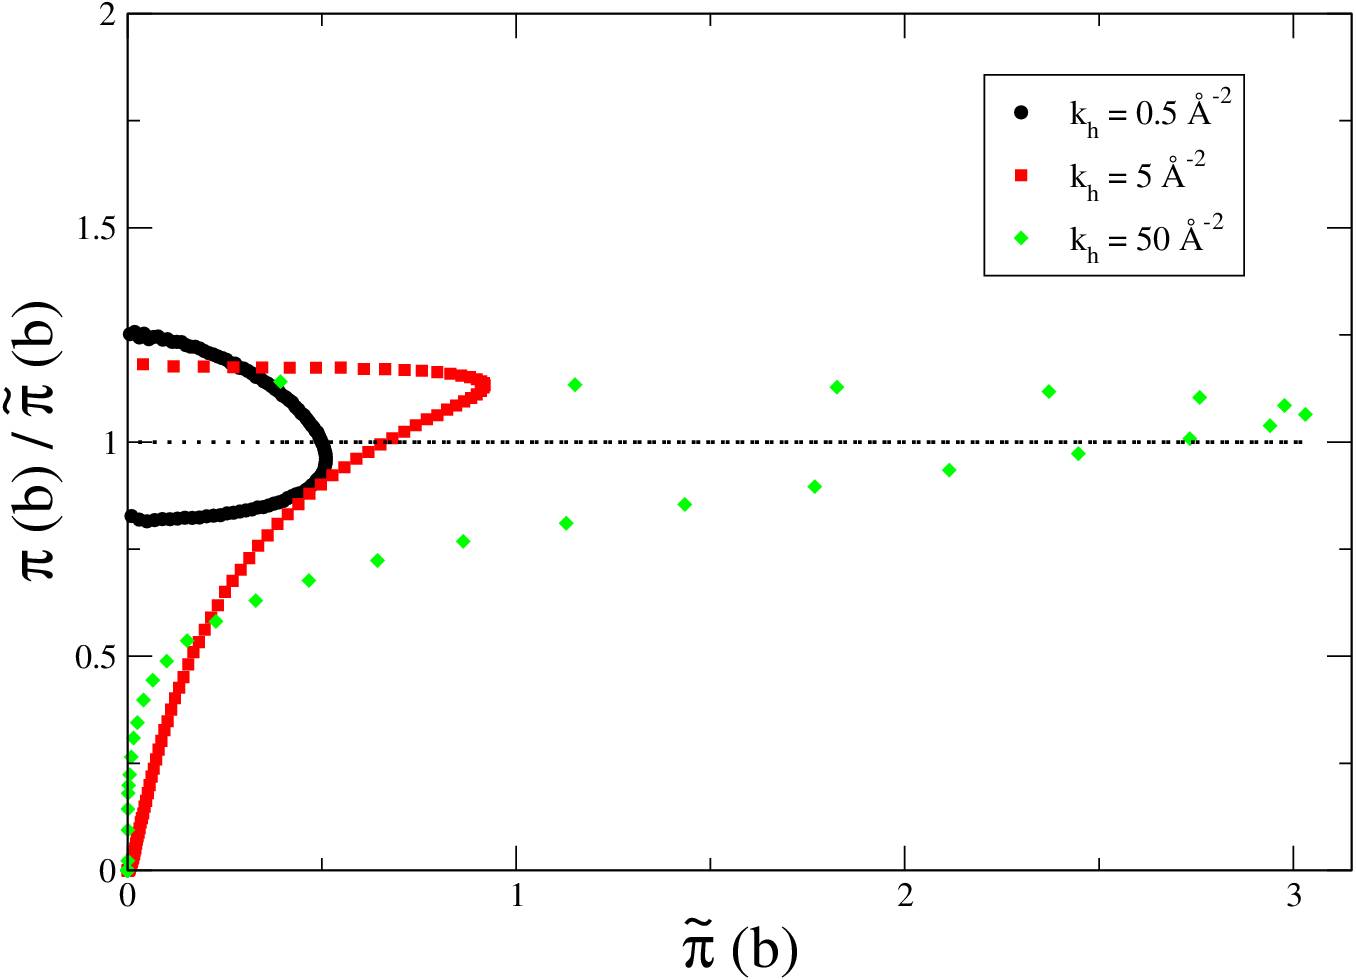
\includegraphics[scale=0.20,keepaspectratio]{Chapter-4/Figures/ratio8B.png}
                    \caption{Ratio of the approximate and actual probability distributions for $P' =$ 8.}
                    \label{fig:ratio8B}
                \end{figure}

                From figs. \ref{fig:ratio2B}, \ref{fig:ratio4B} and \ref{fig:ratio8B}, we can infer the following:
                \begin{itemize}
                    \item In some cases, ``closeness" (as defined above) of the intermediate $k_h$ (= 5 \AA$^{-2}$) is worse than the other two cases. This could lead to the minimum in fig. \ref{fig:r0Acc} because $k_h$ is directly proportional to temperature. It is worth noting that although for one particular image the approximate distribution could be very ``close" to the actual distribution, as we take the product of many such approximate distribution functions the resulting probability distribution function is worse than each individual approximate.
                    \item The points above the $y =$ 1-line indicate  that the actual distribution has been under-predicted by the approximate distribution and these points could potentially lead to configurations where the molecule is `stuck'. In other words, the probability of going from one of these points to a point on the $y =$ 1-line (favored) is very poor. However, this would happen only for $y \gg 1$, which is not observed in any of the hypothetical cases.
                \end{itemize}

        \subsection{Flexible-bond models -- Orientation and bond length trials}
            In this section we present and analyze the results for Model 3 (flexible-bond model) including the performance of the orientation-sampling trial and the bond length sampling trial when present simultaneously in a simulation. We begin by noting that the number of images used by Garberoglio for achieving converged results \cite{Garberoglio2014} for Model 3 was calculated as:
            \begin{equation}
            \label{eq:s3P}
                P = \lceil 7000 K/T + 8 \rceil
            \end{equation}
            where $\lceil x \rceil$ denotes the smallest integer larger than $x$.
            
            According to Eq. \eqref{eq:s3P} the temperature at which we require $P > 64$ to achieve converged results for Model 3 is 100 K. Therefore we expect to see significant differences between our virial coefficient values for Model 3 and the corresponding reference values for $T \le 100 K$. Although for a given temperature $T$, Eq. \eqref{eq:s3P} provides a good estimate of $P$ required for achieving converged results, in practice, one might be able to achieve convergence with fewer $P$ as well.

            \subsubsection{$B_2$ values}
                \begin{figure}[!htbp]
                    \centering
                    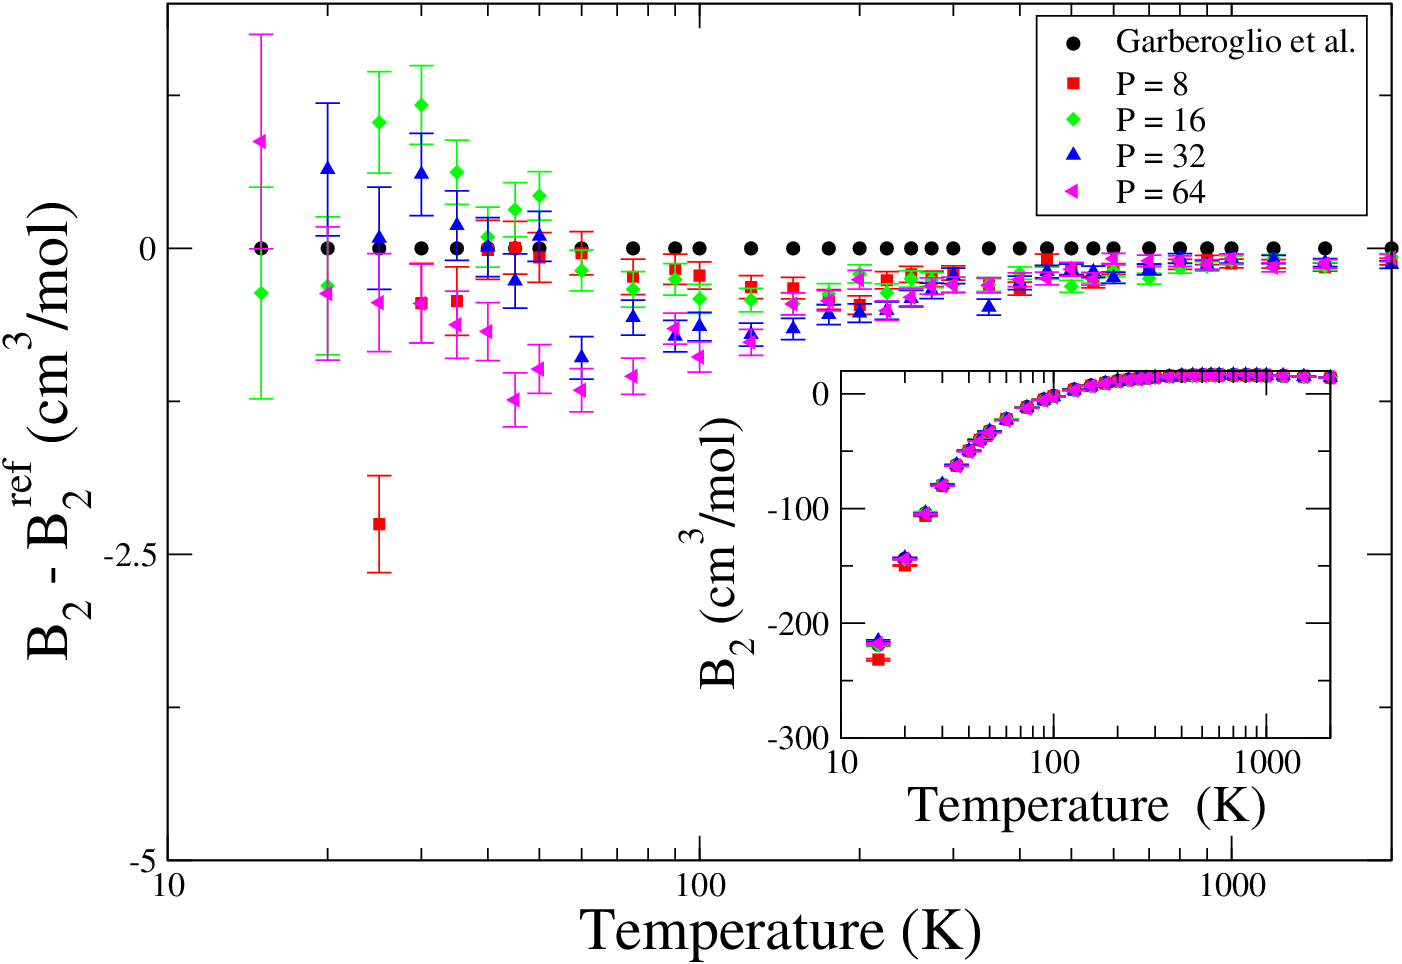
\includegraphics[scale=0.20,keepaspectratio]{Chapter-4/Figures/s3GarberoglioAll.png}
                    \caption{Fully quantum second virial coefficient ($B_2$) values compared against reference values \cite{Garberoglio2014}, for Model 3. Main figure is the difference between the values computed here and the reference values, while the inset shows the coefficients before differencing. The value of the number of path-integral beads is $P$, and the results for different $P$ are as indicated in the legend. Error bars are drawn at $\mu \pm \sigma$ where $\mu$ is the mean value and $\sigma$ is the standard error. It should be noted however, that the 95\% confidence interval is given by $\mu \pm 2\sigma$.}
                    \label{fig:variable}
                \end{figure}
                
                In Fig. \ref{fig:variable} we show our $B_2$ values and the reference values for Model 3 as a function of temperature. It can be seen that the agreement between reference values and our results is generally good over the wide range of temperatures considered (15 K to 2000 K). The agreement is particularly good for $T > 100 K$ where our results using $P = 64$ images are sufficient enough to achieve convergence according to Eq. \eqref{eq:s3P}. For $T \le 100 K$, we observe statistically significant disagreement between our results (for all $P$ considered) and reference values and the magnitude of this deviation decreases with increasing $P$ and/or $T$ and vice-versa. As explained earlier, this behavior is expected because the number of images we use is not sufficient for convergence according to Eq. \eqref{eq:s3P}. It should be noted that in Fig. \ref{fig:r0} the range of the $y$-axis was chosen to highlight the differences over the whole range of temperatures considered and as a result we did not include some data points (whose $B_2$ value was lesser than -5 cm$^3$/mol), especially for low temperatures. However, these data points are for lower-$P$ cases where the virial coefficient values have not yet converged and so we could afford to exclude them from the graphs.
                
            \subsubsection{Orientation algorithm performance}
                \begin{figure}[!htbp]
                    \centering
                    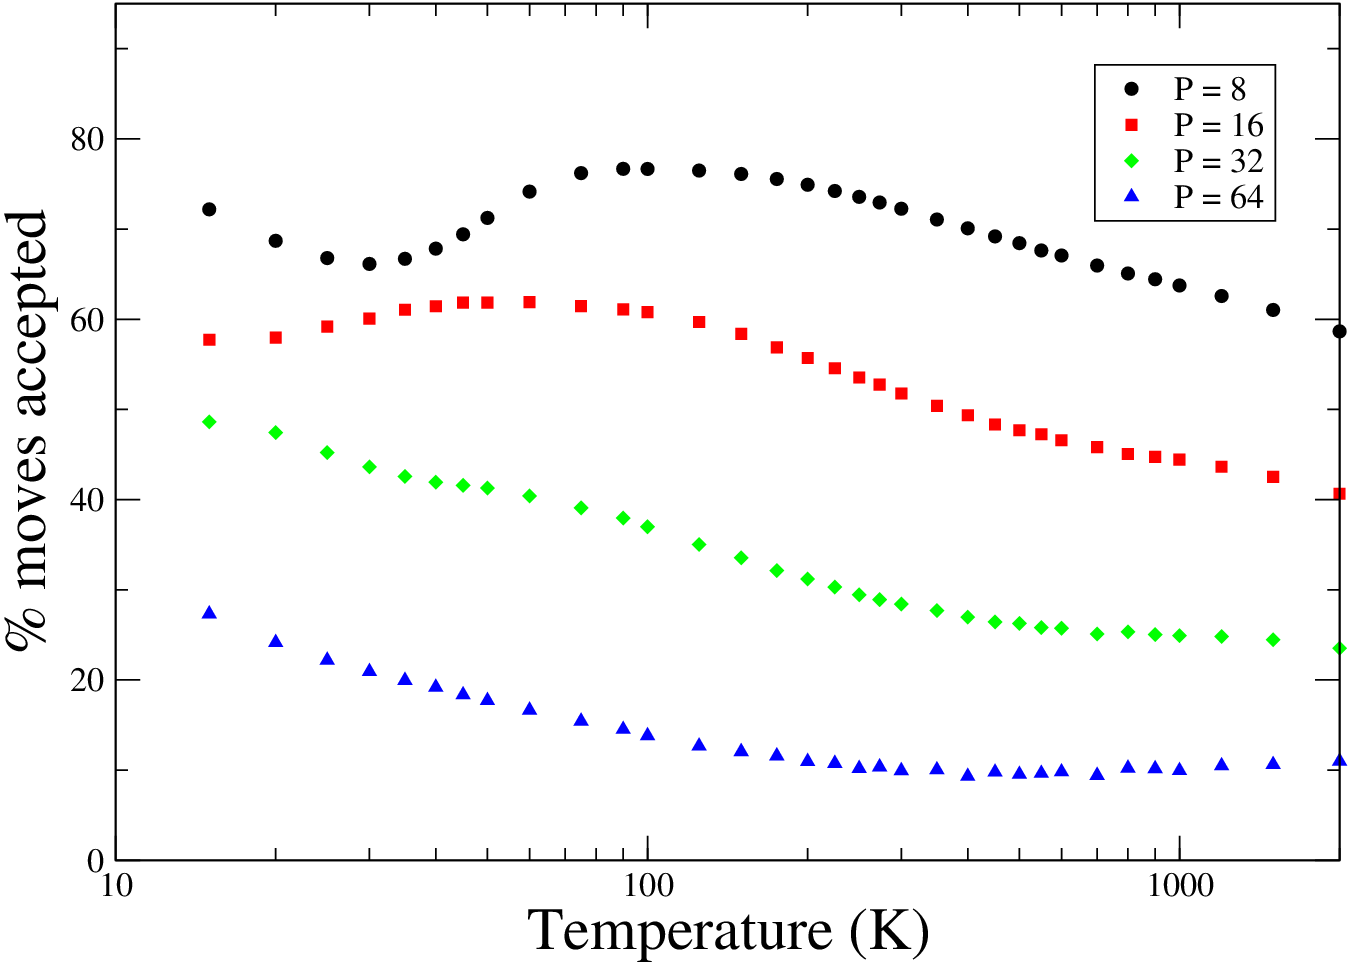
\includegraphics[scale=0.20,keepaspectratio]{Chapter-4/Figures/s3OrAcc.png}
                    \caption{Performance of the orientation move for simulation option $s_3$}
                    \label{fig:variableOrAcc}
                \end{figure}

                In fig. \ref{fig:variableOrAcc} we have shown the percentage of orientation moves that were accepted as a function of temperature for simulation option $s_3$. We notice once again that the algorithm performance decreases with increasing $P$ which is to be expected because of the non-exact nature of the description of the $\alpha$ for $P/2$ images. In addition, we also observe that the performance of the orientation move is almost always worse in the presence of the bond length change move as can be seen in figs. \ref{fig:r0Acc} and \ref{fig:variableOrAcc}. This can be attributed to the way we handle the bond lengths of different images being different within the orientation move. In its current implementation, we average the bond lengths of images $i$ through $k$ and use this value to place image $j$. However, this leads to using the incorrect value of the spring constant when computing the approximate distribution function, which in turn could lead to poor percentage acceptance of the move.

            \subsubsection{Bond length algorithm performance}
                \label{sec:blPerformance}
                Before looking at the performance of the bond length algorithm, we present the following as evidence to support our use of the expression $b_i^{2/P}$ in place of $b_i^2$ in eq. \eqref{eq:ytilde}. We collected histograms of the average adjacent angle $\theta_{ij}$ during the course of $s_1$ simulations for $T = 15, 50, 100, 250$~and $500$ K and for $P = 8, 16, 32$~and $64$.
                \begin{figure}[!htbp]
                    \centering
                    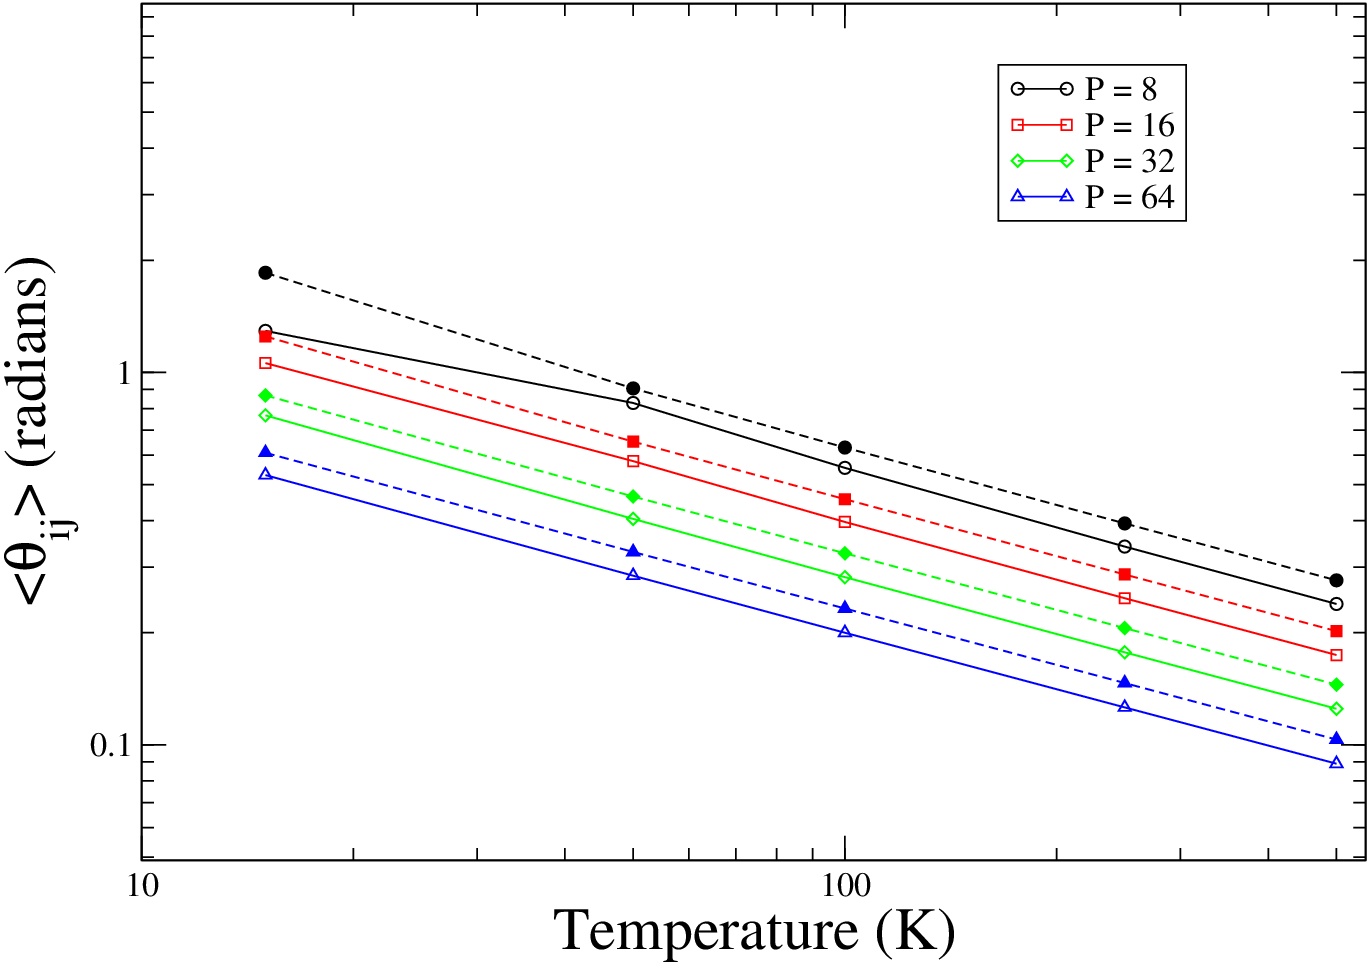
\includegraphics[scale=0.20,keepaspectratio]{Chapter-4/Figures/nominalAnglelogXlogY.png}
                    \caption{Nominal angle computed using eq. \eqref{eq:thetaHat} compared against average $\theta_{ij}$ observed in simulation (Note: both axes are shown in log scale). Open symbols connected by solid lines represent the $<\theta_{ij}>$ observed in simulation and filled symbols with the same shape connected by dashed lines represent the $\hat \theta$ computed using the formula given in eq. \eqref{eq:thetaHat}}
                    \label{fig:nominal_angle}
                \end{figure}

                From fig. \ref{fig:nominal_angle} we can clearly see that although eq. \eqref{eq:thetaHat} over-predicts $<\theta_{ij}>$ slightly for all cases, this would result only in a marginal decrease in the efficiency of the sampling algorithm. Therefore, we assumed it would be a small price to pay when compared to the amount of computational effort saved by not performing the normal mode analysis before each bond length trial.

                \begin{figure}[!htbp]
                    \centering
                    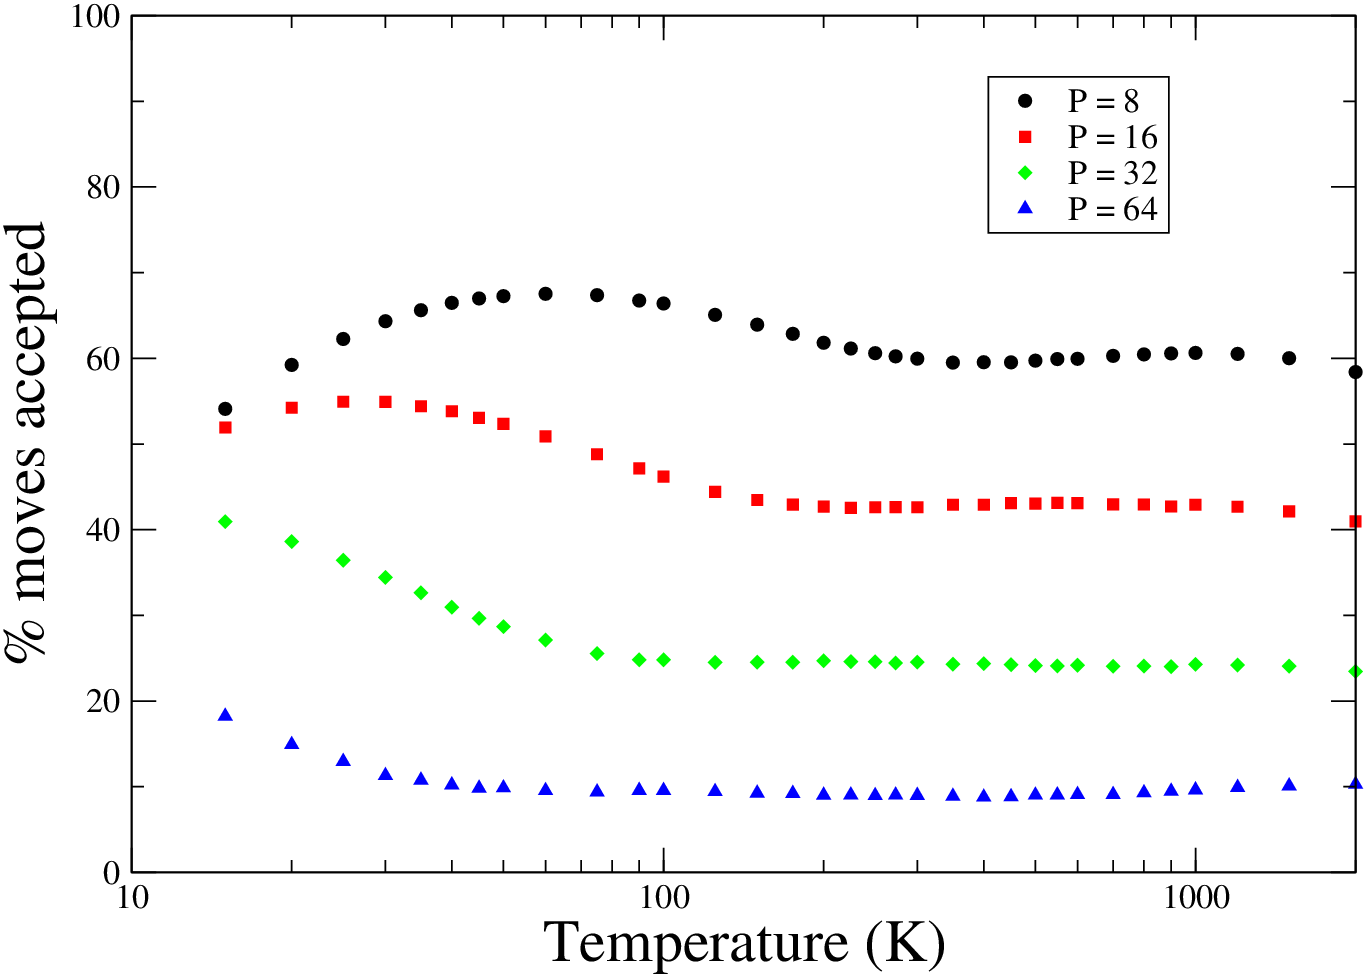
\includegraphics[scale=0.20,keepaspectratio]{Chapter-4/Figures/s3BlAcc.png}
                    \caption{Performance of the bond length move for simulation option $s_3$}
                    \label{fig:variableBlAcc}
                \end{figure}

                In fig. \ref{fig:variableBlAcc} we have shown the percentage of bond length moves that were accepted as a function of temperature for simulation option $s_3$. For a fixed $T$, the percentage acceptance decreases with increasing $P$. Although the approximation of the behavior of the bond lengths to be of Gaussian nature using the normal mode analysis affects the performance of the bond length algorithm, we did not attempt to investigate this further. Neither did we probe alternative approaches to compute the nominal angle $\hat \theta$. For our current purposes, we found the performance of the bond length sampling algorithm to be satisfactory.

                The algorithms developed in Sections \ref{subsec:orMove} and \ref{subsec:blMove} do not involve the use of quantum chemistry calculations and hence allow for considerable efficiency improvements. The mass of the atom that forms the diatomic molecule is used as input to each of the algorithms. Although this allows us to differentiate between different isotopes of the same atom, the algorithms cannot differentiate between the different quantum mechanical spins(i.e., \emph{para}- and \emph{ortho}-H$_2$) of the molecule. Garberoglio et al. \cite{Garberoglio2014} use different number of images $P$, as a means to accomplishing this difference within the PIMC calculation. We have not used the same $P$ as theirs, in order to gauge the performance of our algorithms for different conditions as mentioned above. Therefore, in some cases, we observe large deviations from reference values where the use of larger $P$ is necessary. 

\chapter{Nitrogen}
\label{chap:n2}
\section{Recent developments}
            Experimental second virial coefficients have often complemented \abinitio{} PESs for nitrogen that have resulted in rescaled or improved PESs. With the advent of computational techniques we expect that theory is soon to replace experiments as the source of high quality virial coefficients (see e.g. Shaul et al. \cite{Shaul2012SC} for the case of helium-4). Such highly accurate and precise second virial coefficient data will lead to better quality PESs, using which one can predict thermodynamic, transport, structural and other properties of nitrogen much more accurately. Berns and van der Avoird \cite{Berns1980} reported one of the first \abinitio{} PES (BvdA) for the Nitrogen (${\rm N_2 - N_2}$) dimer including first order exchange, short-range electrostatic contributions and long-range data of Mulder et al. \cite{Mulder1980}. They developed two analytic representations of their calculations: 1) A spherical harmonic expansion and 2) a two site point charge model with a shifted force center. Describing the region near the van der Waals minimum accurately, was one of the primary goals of their work. The BvdA potential was used to study crystal structure properties \cite{Luty1980} and transport properties \cite{Nyeland1984}. Whereas the long-range interaction calculations performed by Mulder et al. \cite{Mulder1980} were obtained using uncoupled HF method, Visser et al. \cite{Visser1983} performed time-dependent coupled HF method and consequently reported more accurate long-range interaction coefficients. Ad van der Avoird et al. \cite{vanDerAvoird1986} reported a new potential(AWJ) by including these improved long-range coefficients and more basis sets. However, it was observed that the van der Waal well prediction of the potential was too shallow. This resulted in large discrepancies between the calculated second virial coefficient values and the experimentally observed results. Neglect of intramolecular electron correlation leading to significant short-range exchange repulsion in the intermolecular potential was identified and later confirmed to be the possible cause for this discrepancy. Therefore, they introduced two scaling constants to change the size and slope of the short-range exchange repulsion term to obtain a rescaled potential that yielded second virial coefficients that were in much better agreement with experiments. Highly accurate experimental virial coefficient data sets were used to improve \abinitio{} PES obtained as a result of calculations performed at the CCSD(T) level with large basis sets by Stallcop et al. \cite{Stallcop1997}. A semi-empirical relation between the parameters of the repulsive potential and the accurate virial coefficient data sets was also reported. Cappelletti et al. \cite{Cappelletti1998} also reported a potential which was an improvement of the AWJ potential, by firstly computing \abinitio{} PES at the CCSD(T) level of theory and then using accurate data from scattering, virial coefficients and other property measurements to improve the PES quality. An extensive \abinitio{} study was conducted by Leonhard et al. \cite{Leonhard2002} to not only develop a improved 2-body potential but also to analyze two 3-body potentials for their capability to reproduce thermodynamic properties if both the 2-body as well as 3-body potentials were used. The 2-body \abinitio{} PES was rescaled to fit accurate second virial coefficient data. After comparison to experimental results, the 3-body potential due to Axilrod Teller (AT) \cite{Axilrod1943} performed better than the one due to Stogryn \cite{Stogryn1969}, when used in combination with the 2-body potential. Gomez et al. \cite{Gomez2007} reported an \abinitio{} PES that was calculated using SAPT. The accuracy of perturbative energies were compared against calculations at the CCSD(T) level of theory using large basis sets. They observed better agreement to experimental virial coefficients than previous unscaled PESs for the range of temperatures investigated. They attributed the consistently lower second virial coefficient predictions by using their PES, to possible overestimation of the van der Waal's well within their calculations. Str\k{a}k et al. \cite{Strak2007} also performed \abinitio{} calculations at the CCSD(T) level of theory that resulted in a potential that was used in combination with Molecular Dynamics (MD) simulations to obtain an equation of state for the dimer. The resulting predictions of physical properties based on this equation of state were found to be in excellent agreement with experiments for a wide range of temperatures (up to 2000K) and pressures (up to 30GPa). Hellmann \cite{Hellmann2013} recently performed \abinitio{} calculations at the CCSD(T) level of theory using basis sets up to aug-cc-pV5Z supplemented with bond functions. The resulting 2-body (scaled) and 3-body potential was used to compute second and third (including 3-body effects) virial coefficients that were most accurate with experiments than previously reported values.
\section{Computational details}
    \subsection{Second virial coefficients}
    \label{subsubsec:b2n2}
        The \abinitio{} potential (denoted as $U_2^H$) that we used was due to Hellmann \cite{Hellmann2013}. We have performed classical and semi-classical virial coefficient calculations, each using $10^9$ configuration samples and two types of MC trials 1) translation and 2) rotation of the dimer. Instead of using the semi-classical TI version of the Hellmann potential, we have used the semi-classical QFH version of the potential which is given as follows \cite{Feynman,Schenter2002}:
        \begin{equation}
        \label{eq:QFH}
            U_2^{\rm QFH} = U_2^H + \displaystyle\frac{\hbar^2 \beta}{24 m} \Big[ \pmb{\nabla}^2 U_2^H + \frac{2}{r} \pmb{\nabla} U_2^H \Big].
        \end{equation}

        This was done based on some preliminary calculations that we carried out where we failed to observe any significant improvement in the precision of the results while using the semi-classical TI version of $U_2^H$ (which was done by Hellmann). Therefore we expect significant differences while comparing our virial coefficient values for the semi-classical calculations against Hellmann's, especially at low temperatures. We have performed PIMC calculations using $P$ = 8, 16, 32 and 64 classical images for each of the temperatures reported by Hellmann and collected $10^8$ configuration samples each. Apart from the translation of the dimer, we also include MC trials to regrow the ring by translating the beads (see Sec. \ref{subsec:orMove}) and our recently developed orientation algorithm (cite:hydrogen) (explained in Sec. \ref{subsec:orMove}). We have performed PIMC calculations using semi-classical images and also the exact same conditions as PIMC with classical beads that are mentioned above. We note that for this calculation, we employed the TI propagator (Eq. \eqref{eq:TI}).

    \subsection{Third virial coefficients}
        We repeated all the calculations under the same conditions (except the semi-classical additive as well as non-additive calculations for which we used $10^8$ configuration samples as opposed to $10^9$ for the second virial coefficient case) that were explained in Sec. \ref{subsubsec:b2n2} for computing the additive as well as non-additive contributions to the third virial coefficients. It should be noted that we employed the non-additive 3-body potential that was also reported by Hellmann \cite{Hellmann2013} to compute the non-additive contributions. Also, we performed the semi-classical additive as well as non-additive simulations using the same QFH version of $U_2^H$ as in Eq. \eqref{eq:QFH}. We note that all the third virial coefficient simulations were performed at a set of 90 temperatures considered by Hellmann.
\section{Results and discussion}
    \subsection{Second virial coefficients}
        In order to reproduce the results of Hellmann and to ensure that our implementation of the \abinitio{} potential was correct, we performed classical virial coefficient calculations as a first step. In Fig. \ref{fig:B2CLN2} we show the difference, between our results and Hellmann's for the second virial coefficient as a function of temperature, in the main plot and show the actual values in the inset plot, also as a function of temperature.
        \begin{figure}[!htbp]
            \centering
            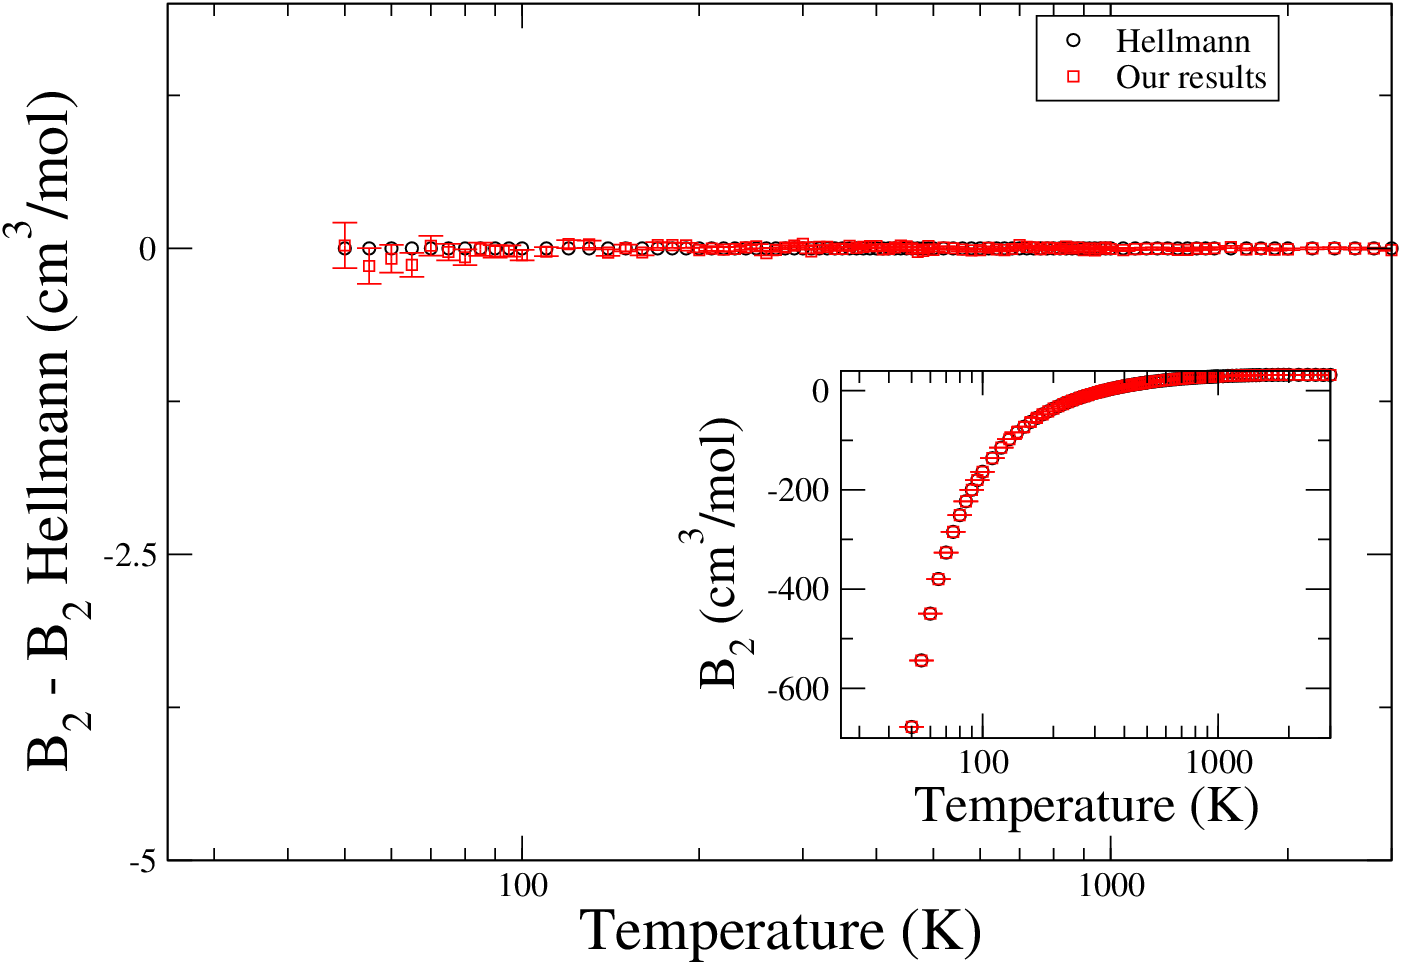
\includegraphics[scale=0.20,keepaspectratio]{Chapter-5/Figures/B2CL9sResultsAll.png}
            \caption{Classical second virial coefficient ($B_2$) values compared against Hellmann's values \cite{Hellmann2013}. Error bars are drawn at $\mu \pm \sigma$ where $\mu$ is the mean value and $\sigma$ is the standard error. It should be noted however, that the 95\% confidence interval is given by $\mu \pm 2\sigma$.}
            \label{fig:B2CLN2}
        \end{figure}
        It can be clearly seen from Fig. \ref{fig:B2CLN2} that our classical results are in excellent statistical agreement with Hellmann's for the entire range of temperatures, suggesting that our implementation of the \abinitio{} potential is correct.

        In Fig. \ref{fig:B2SCN2} we show the difference between, our semi-classical second virial coefficient results and Hellmann's as a function of temperature, in the main plot and show the actual values in the inset plot, also as a function of temperature.
        \begin{figure}[!htbp]
            \centering
            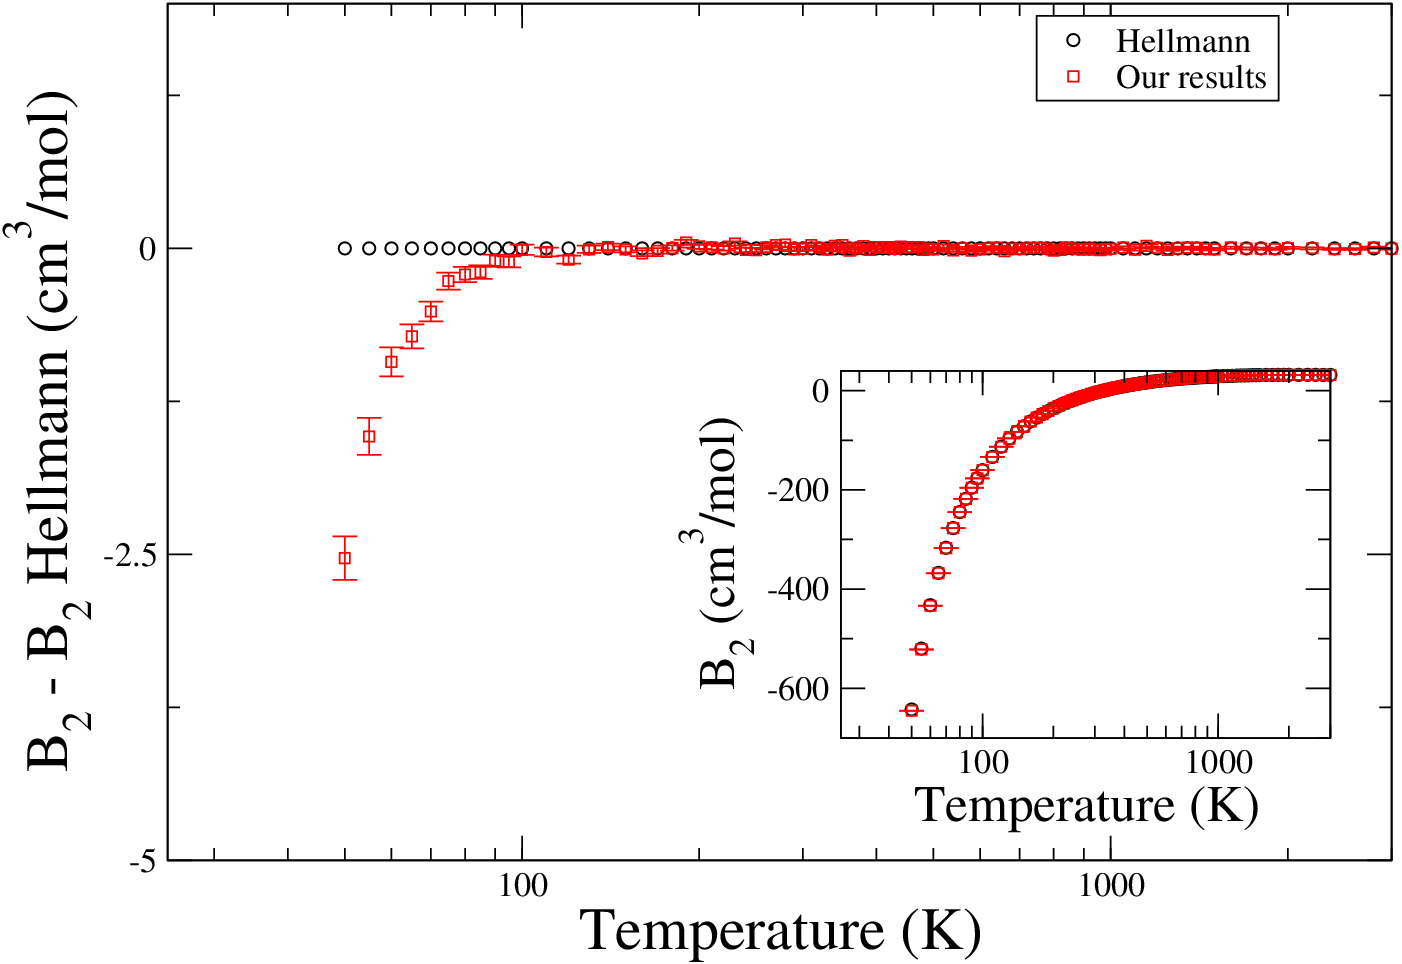
\includegraphics[scale=0.20,keepaspectratio]{Chapter-5/Figures/B2SC9sResultsAll.png}
            \caption{Semi-classical second virial coefficient ($B_2$) values compared against Hellmann's values \cite{Hellmann2013}. Error bars are drawn at $\mu \pm \sigma$ where $\mu$ is the mean value and $\sigma$ is the standard error. It should be noted however, that the 95\% confidence interval is given by $\mu \pm 2\sigma$.}
            \label{fig:B2SCN2}
        \end{figure}
        From Fig. \ref{fig:B2SCN2} and the argument made in Sec. \ref{subsubsec:b2n2}, we can clearly see that our semi-classical results are in excellent agreement with Hellmann's for temperatures $T \ge 100K$. The deviation observed for lower temperatures can be explained by the use of a different semi-classical form of the intermolecular function, i.e., whereas we have used the semi-classical QFH version (Eq. \eqref{eq:QFH}) , Hellmann used the semi-classical TI version (Eq. \eqref{eq:TI}) of the \abinitio{} potential. From Fig. \ref{fig:B2SCN2} one can also make the observation that the semi-classical QFH and the TI versions of the \abinitio{} PES produce similar results until about $T = 100K$ where we start noticing significant deviations.

        In Fig. \ref{fig:B2AllDiffPICB} we plot the differences between the quantum virial coefficient values computed using classical beads and the case of semi-classical beads with $P$ = 64. Under the reasonable assumption that the PI-SCB approach with $P$ = 64 yields the most accurate value, we compare the values computed using PI-CB approaches for different $P$. From Fig. \ref{fig:B2AllDiffPICB}, we can see that there is not much noticeable improvement for the PI-SCB approach over the PI-CB approaches, suggesting that for the purpose quantum virial calculations, we need not resort to PI-SCB approaches.
        \begin{figure}[!htbp]
            \centering
            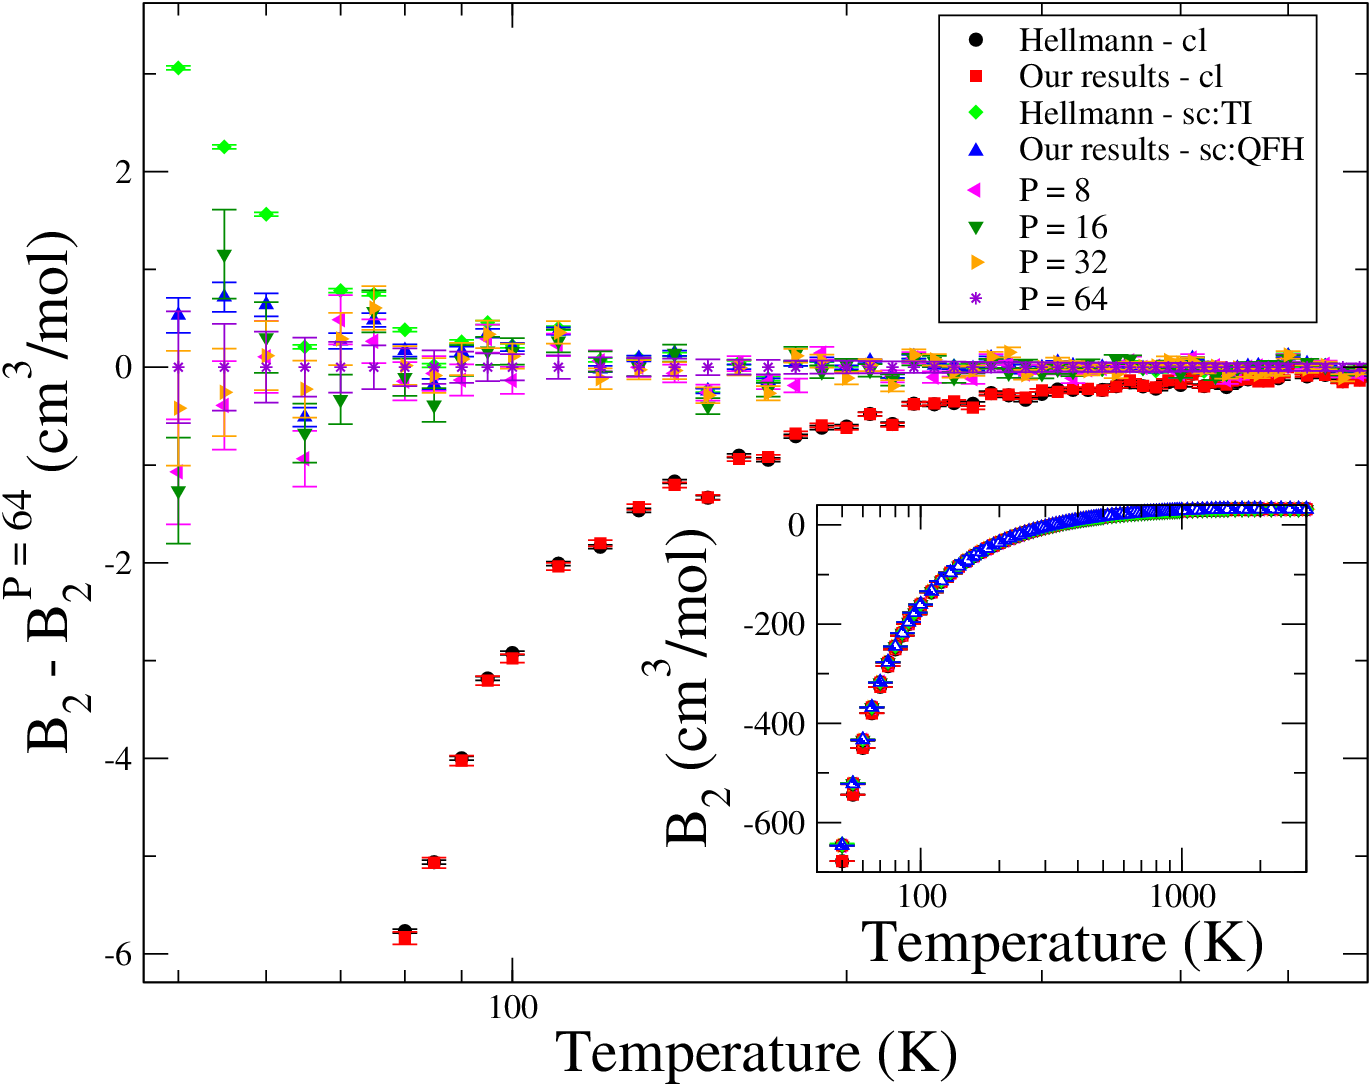
\includegraphics[scale=0.20,keepaspectratio]{Chapter-5/Figures/B2AllDiffPICB.png}
            \caption{Difference between second virial coefficients computed with PI using CB approaches and PI using SCB approach with $P$ = 64 images.}
            \label{fig:B2AllDiffPICB}
        \end{figure}

    \subsection{Third virial coefficients}
        In Figs. \ref{fig:B3CLN2} and \ref{fig:B3SCN2}, we plot the classical and the semi-classical third virial coefficients including additive and non-additive contributions. It should be noted that the range of the $y$-axes were chosen to highlight the differences over the whole range of temperatures considered and as a result we did not include some data points (whose $B_3$ value was lesser than -5 cm$^6$ mol$^{-2}$), especially for low temperatures.
        \begin{figure}[!htbp]
            \centering
            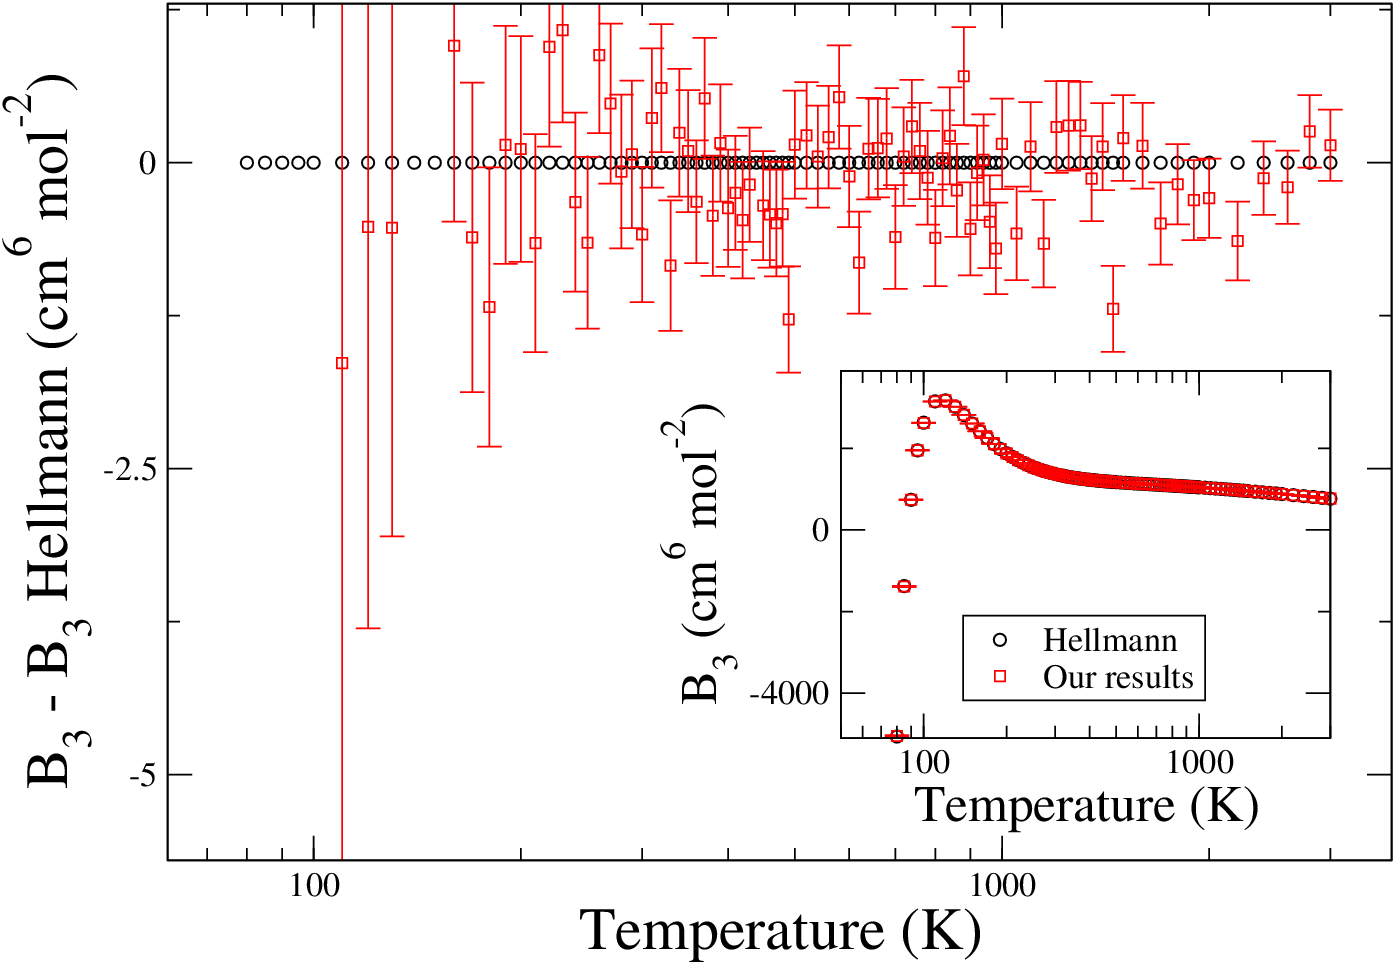
\includegraphics[scale=0.20,keepaspectratio]{Chapter-5/Figures/B3CLFull9sResultsAll.png}
            \caption{Classical second third coefficient ($B_3$) values compared against Hellmann's values \cite{Hellmann2013}. Error bars are drawn at $\mu \pm \sigma$ where $\mu$ is the mean value and $\sigma$ is the standard error. It should be noted however, that the 95\% confidence interval is given by $\mu \pm 2\sigma$.}
            \label{fig:B3CLN2}
        \end{figure}

        \begin{figure}[!htbp]
            \centering
            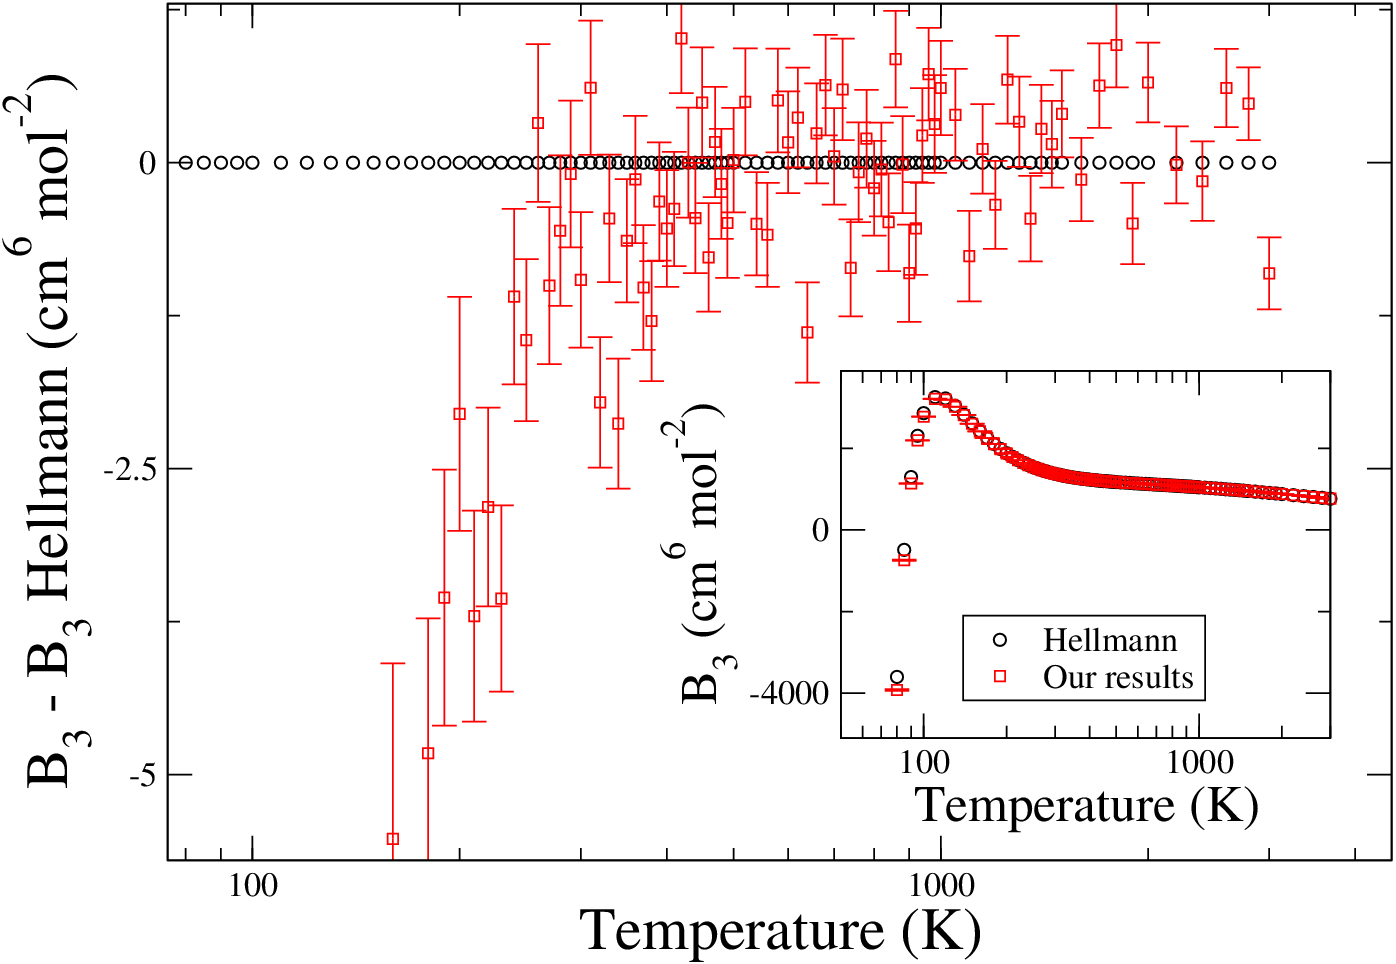
\includegraphics[scale=0.20,keepaspectratio]{Chapter-5/Figures/B3SCFull8sResultsAll.png}
            \caption{Semi-classical third virial coefficient ($B_3$) values compared against Hellmann's values \cite{Hellmann2013}. Error bars are drawn at $\mu \pm \sigma$ where $\mu$ is the mean value and $\sigma$ is the standard error. It should be noted however, that the 95\% confidence interval is given by $\mu \pm 2\sigma$.}
            \label{fig:B3SCN2}
        \end{figure}

        From Fig. \ref{fig:B3CLN2}, we see that our classical $B_3$ results agree quite well with Hellmann's for the entire range of temperatures considered (except a few outliers). The standard error of our results seem to be decreasing with increasing temperature and this is to be expected because any system approaches classical behavior at high enough temperatures. From Fig. \ref{fig:B3SCN2}, we can see that there is quite a bit of deviation of our semi-classical results from Hellmann's corresponding results for $T \le 300K$. As explained earlier, this might be attributed to the use of a different semi-classical form of the \abinitio{} potential. It can also be seen that the deviations become less significant for $T > 300K$. 
        
        In Fig. \ref{fig:B3AllDiffPICB} we plot the differences between the quantum virial coefficient values computed using classical beads and the case of semi-classical beads with $P$ = 64. Under the reasonable assumption that the PI-SCB approach with $P$ = 64 yields the most accurate value, we compare the values computed using PI-CB approaches for different $P$. From Fig. \ref{fig:B3AllDiffPICB}, we can see that there is not much noticeable improvement for the PI-SCB approach over the PI-CB approaches, suggesting that for the purpose quantum virial calculations, we need not resort to PI-SCB approaches.
        \begin{figure}[!htbp]
            \centering
            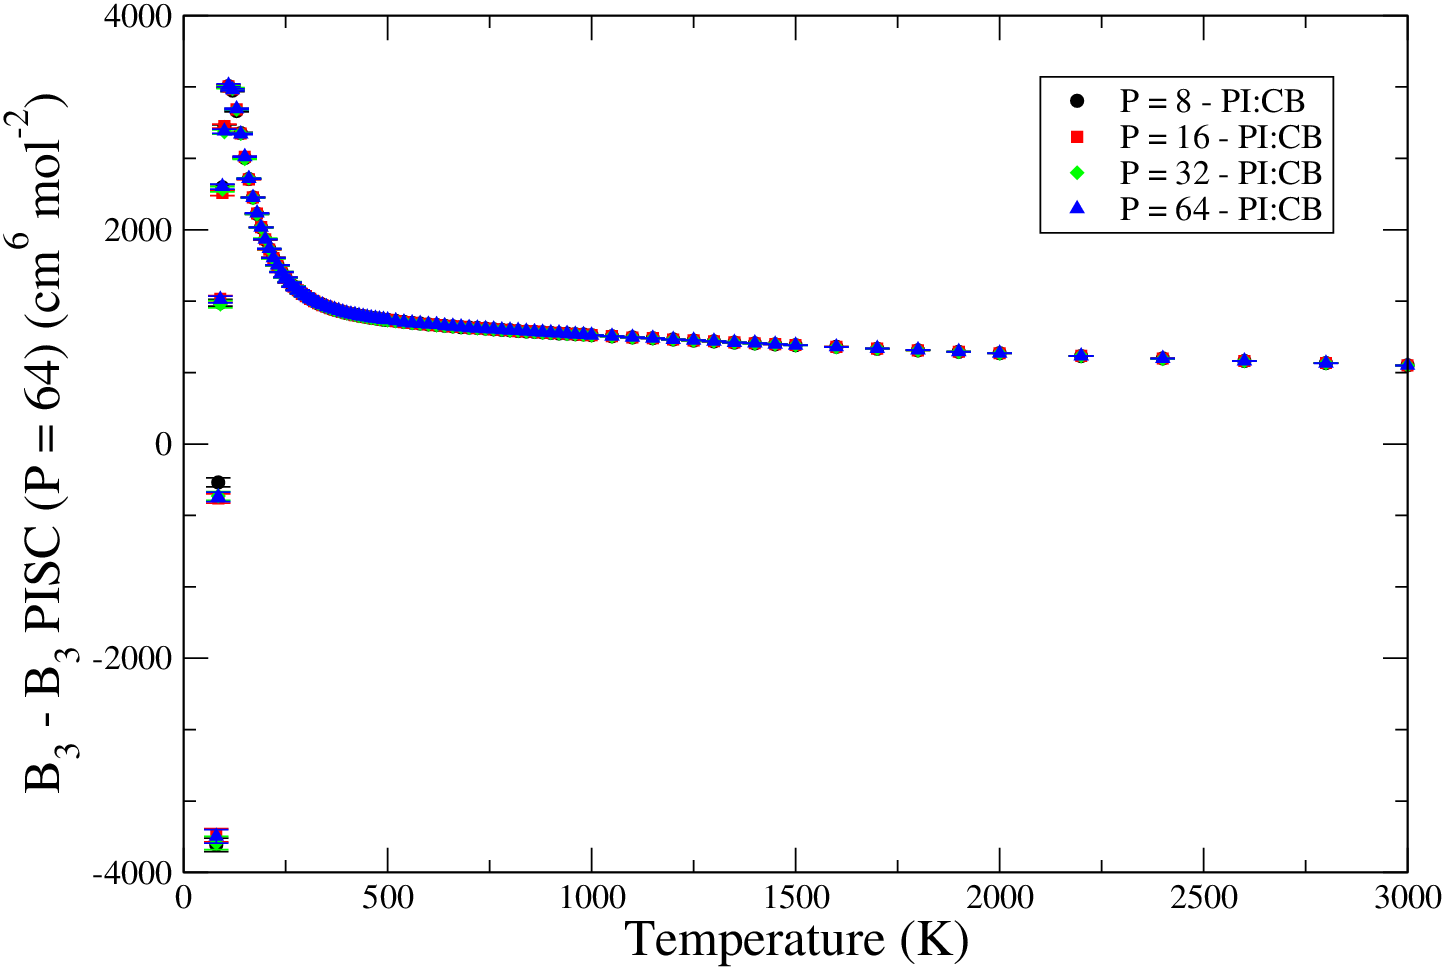
\includegraphics[scale=0.20,keepaspectratio]{Chapter-5/Figures/B3AllDiffPICB.png}
            \caption{Difference between second virial coefficients computed with PI using CB approaches and PI using SCB approach with $P$ = 64 images.}
            \label{fig:B3AllDiffPICB}
        \end{figure}
    
    \section{Conclusions}
    \label{sec:conclusion}
        We have calculated fully quantum virial coefficients for nitrogen dimers by explicitly including nuclear quantum effects via PIMC method. Additionally, we have calculated fully quantum virial coefficients for the nitrogen dimer using PIMC with semi-classical beads, an approach that was recently (cite:helium) introduced. Based on our results, we have concluded that for the purpose of quantum second virial coefficient calculations, the utilization of semi-classical beads does not provide any significant improvement over the classical beads in terms of faster convergence and better precision. We have also employed a new algorithm that we recently (cite:hydrogen) developed to sample orientations of diatomic molecules, in all our PIMC calculations. We have compared our PIMC results against the most accurate data available in literature and found excellent agreement. As a result of this work, the validity and robustness of the orientation sampling algorithm have been successfully tested.

\chapter{Oxygen}
\label{chap:o2}
\section{Recent developments}
    \Abinitio{} studies for the ${\rm O_2 - O_2}$ system are computationally difficult due to the open shell nature of the monomer $\rm{O_2}$ which prevents the orthogonalization of the monomer wavefunctions \cite{Bussery1993}. Recently it is gaining popularity in the field of buffer gas cooling and trapping of oxygen \cite{Friedrich1998,Avdeenkov2001}. Since the ground state monomer exists in the triplet state, there are three possible molecular spin states (denoted as singlet, triplet and quintet) and associated \PESs{}. The short-range exchange interactions were known to cause not only repulsion but also splitting between the molecular spin states of the dimer. Computationally expensive short-range exchange calculations using the Heisenberg Hamiltonian were first performed by van Hemert et al. \cite{vanHemert1983} in a preliminary study and later by Wormer and van der Avoird \cite{Wormer1984}. The authors reported \abinitio{} calculations including electrostatic as well as exchange interactions but excluding long range dispersion interactions as they were primarily interested in studying the solid phase magnetic properties of the dimer. They reported \PESs{} for the three different spin states using spherical expansion to represent the orientational dependence and exponential functions to represent the dependence on intermolecular distance.  By including first order electrostatic and exchange contributions \abinitio{}, second order polarization energy semi-empirically, Bussery and Wormer \cite{Bussery1993} reported improved \PESs{} for the oxygen dimer and used it mainly for studying optical properties. By accounting for dipole-dipole as well as multipole-multipole contributions, they were able to accurately capture the intermolecular correlation energy. The simple analytic form of the polarization energy helped improve their overall computational efficiency as well. The gas phase second virial coefficients computed using the different \PESs{} were found to be in very good statistical agreement with experiments. Really precise molecular beam experiments were performed by Aquilanti et al. \cite{Aquilanti1999} to obtain anisotropic \PESs{} using a spherical harmonics expansion but including only four terms. This led to a simplified potential model with less number of fitted parameters. Upon comparison with the \abinitio{} calculations of Bussery et al. \cite{Bussery1993}, they found good agreement for various geometrical predictions related to the dimer structure. Hernández-Lamoneda et al. \cite{Lamoneda2005CPL} in a preliminary study and later Bartolomei et al. \cite{Bartolomei2008} performed really accurate \abinitio{} calculations at RCCSD(T) level of theory for the quintet state of the oxygen dimer. This was possible only for the quintet state because of the acceptable nature of a single configuration reference as the zeroth-order function. Such highly accurate calculations are not possible for the singlet and triplet states. However, MRCI calculations, albeit with size inconsistency issues can still be applied to study these states. By accurately extracting the spin-coupling parameter $J$ involved in the Heisenberg Hamiltonian within the MRCI calculations and combining it with accurate spin-averaged interaction potential from the RCCSD(T) calculations, they were able to obtain high quality \PESs{} than previous studies. Zuchowski \cite{Zuchowski2008} performed SAPT based DFT calculations for the quintet state and observed very good agreement with previous accurate \abinitio{} coupled-cluster calculations. More recently Bartolomei et al. \cite{Bartolomei2010} have obtained completely \abinitio{} \PESs{} for the three spin states by combining their previous RCCSD(T) data \cite{Bartolomei2008} for the quintet state with new \abinitio{} calculations at the CASPT2 and MRCI levels of theory for the singlet and triplet states. By including dynamical electron correlation at higher levels of theory than previous calculations, they were able to improve the accuracy of the \PESs{}. They observed very good agreement with experiments for their second virial coefficients as well as integral cross sections.
\section{Computational details}
    The \abinitio{} potentials for the different spin multiplicities (s = 0, 1 and 2) and using different levels of theory i.e. MRCI and PT2 were due to Bartolomei et al. \cite{Bartolomei2010}. As we can see, we have 6 different potential surfaces that were reported. The full dimer virial coefficients are obtained for each level of theory by combining the individual spin virial coefficient value according to the formula \cite{Aquilanti1999,Bartolomei2010}:
    \begin{equation}
        B_2 = \frac{B_2^0 + 3 B_2^1 + 5 B_2^2}{9}.
    \end{equation}
    where $B_2^s$ represents the second virial coefficient value computed using the appropriate potential based on the level of theory and the spin multiplicity $s$.

    We have performed classical and PIMC virial coefficient simulations at both levels of theory, all the spin multiplicities and set of 15 temperatures reported. For each type of classical simulation, we have collected $10^8$ configuration samples that were generated using two types of MC trials 1) translation and 2) rotation of the dimer. The PIMC simulations involved $P$ = 8, 16, 32 and 64 images for each condition mentioned above and we collected $10^7$ configuration samples per PIMC simulation. Apart from the translation of the dimer, we also include MC trials to regrow the ring by translating the beads (see Sec. \ref{subsec:orMove}) and our recently developed orientation algorithm (cite:hydrogen) (explained in Sec. \ref{subsec:orMove}).

    To avoid nonphysical values of the intermolecular energy for oxygen dimers, an artificial hard core with a diameter of 4.5 Bohr was used in all virial coefficient calculations. All the oxygen MSMC simulations involved a Hard Sphere reference with a diameter of 4.5 \AA.
\section{Results and discussion}
    We have computed classical as well as quantum virial coefficients using PIMC with $P$ = 8, 16, 32 and 64 images for both the MRCI and the PT2 \PESs{}. In general, our classical and PIMC results agree well with those of Bartolomei et al. \cite{Bartolomei2010} for the, albeit small range of, temperatures considered. In Fig. \ref{fig:B2O2AllDiffMRCI} we plot the difference between various second virial coefficient values and our most accurate PIMC results ($P$ = 64), for the MRCI \PESs{}, as a function of temperature. It should be noted that the range of the $y$-axis was chosen to highlight the differences over the whole range of temperatures considered and as a result we did not include some data points (whose $B_2$ value was lesser than -5 cm$^3$ mol$^{-1}$), especially for low temperatures. 
    \begin{figure}[!htbp]
        \centering
        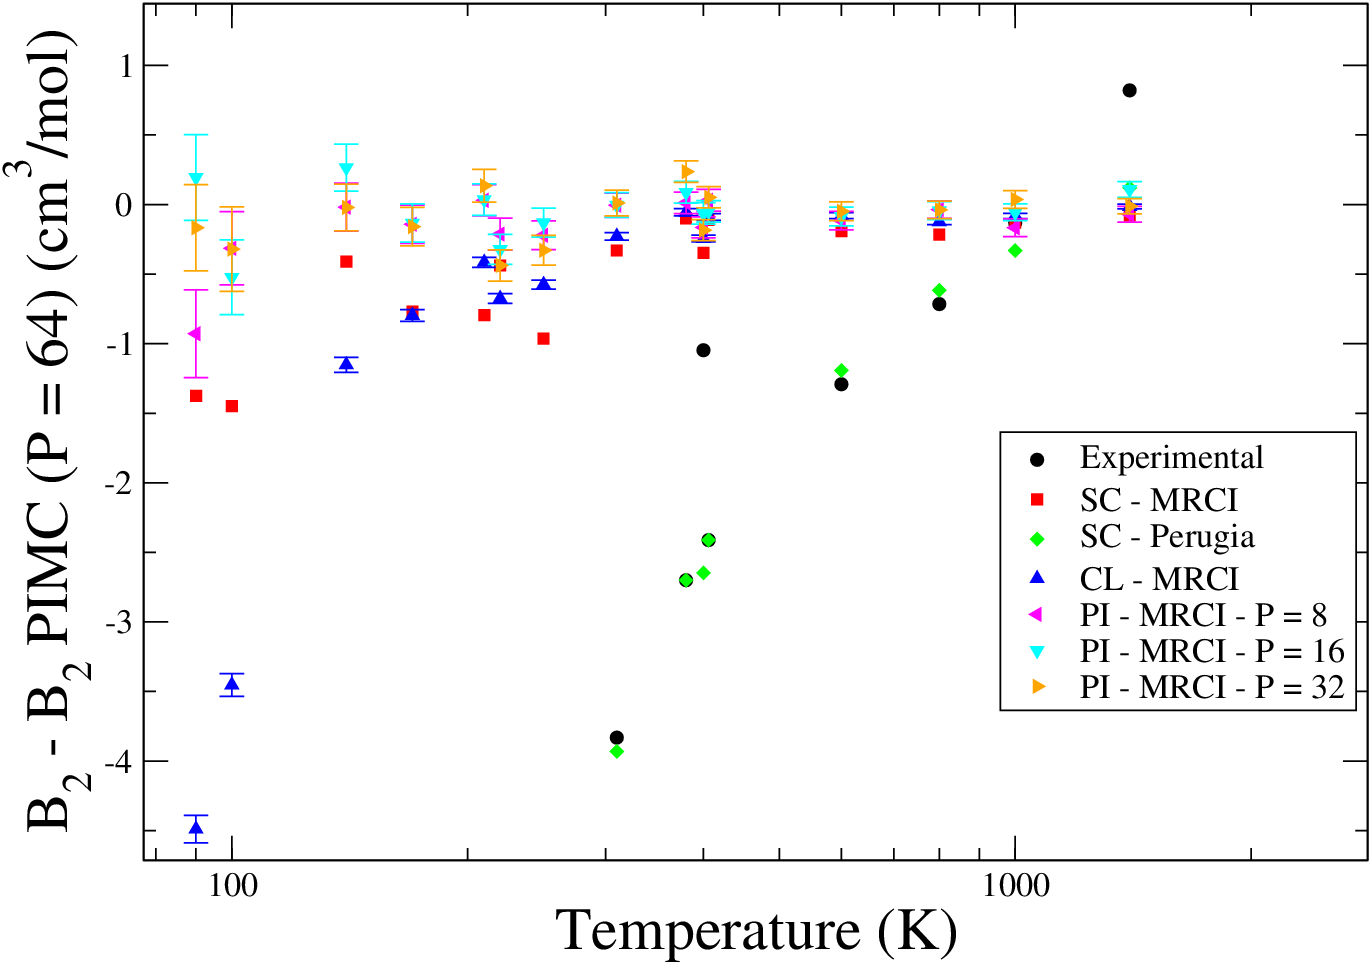
\includegraphics[scale=0.20,keepaspectratio]{Chapter-6/Figures/B2O2AllDiffMRCI.png}
        \caption{Difference between various second virial coefficient ($B_2$) values compared against our most accurate PIMC results ($P$ = 64). Experimental results are from Refs. \cite{Bartolomei2010,Dymond}; SC - MRCI and SC - Perugia are from semi-classical results of Bartolomei et al. \cite{Bartolomei2010} by using the MRCI and Perugia \PESs{} \cite{Aquilanti1999} respectively; CL - MRCI and PI - MRCI are our classical and PIMC results respectively using the MRCI \PESs{}.}
        \label{fig:B2O2AllDiffMRCI}
    \end{figure}

    From Fig. \ref{fig:B2O2AllDiffMRCI}, it can be seen that the semi-classical MRCI calculations performed by Bartolomei et al. \cite{Bartolomei2010} agrees with our PIMC calculations for the same \PESs{}, better than other semi-classical or classical calculations. Additionally, our PIMC calculations have converged for almost all temperatures investigated. Also, the experimental and the SC-Perugia values deviate the largest. For SC-Perugia calculations, this can be explained by the fact that their values are outdated and also because the use of different \PESs{} than ours. Finally, we can see that our classical values start to deviate significantly from the PIMC results for temperatures $T \le 200K$.
    
    In Fig. \ref{fig:B2O2AllDiffPT2} we plot the difference between various second virial coefficient values and our most accurate PIMC results ($P$ = 64), for the PT2 \PESs{}, as a function of temperature. It should be noted that the range of the $y$-axis was chosen to highlight the differences over the whole range of temperatures considered and as a result we did not include some data points (whose $B_2$ value was lesser than -5 cm$^3$ mol$^{-1}$), especially for low temperatures. 
    \begin{figure}[!htbp]
        \centering
        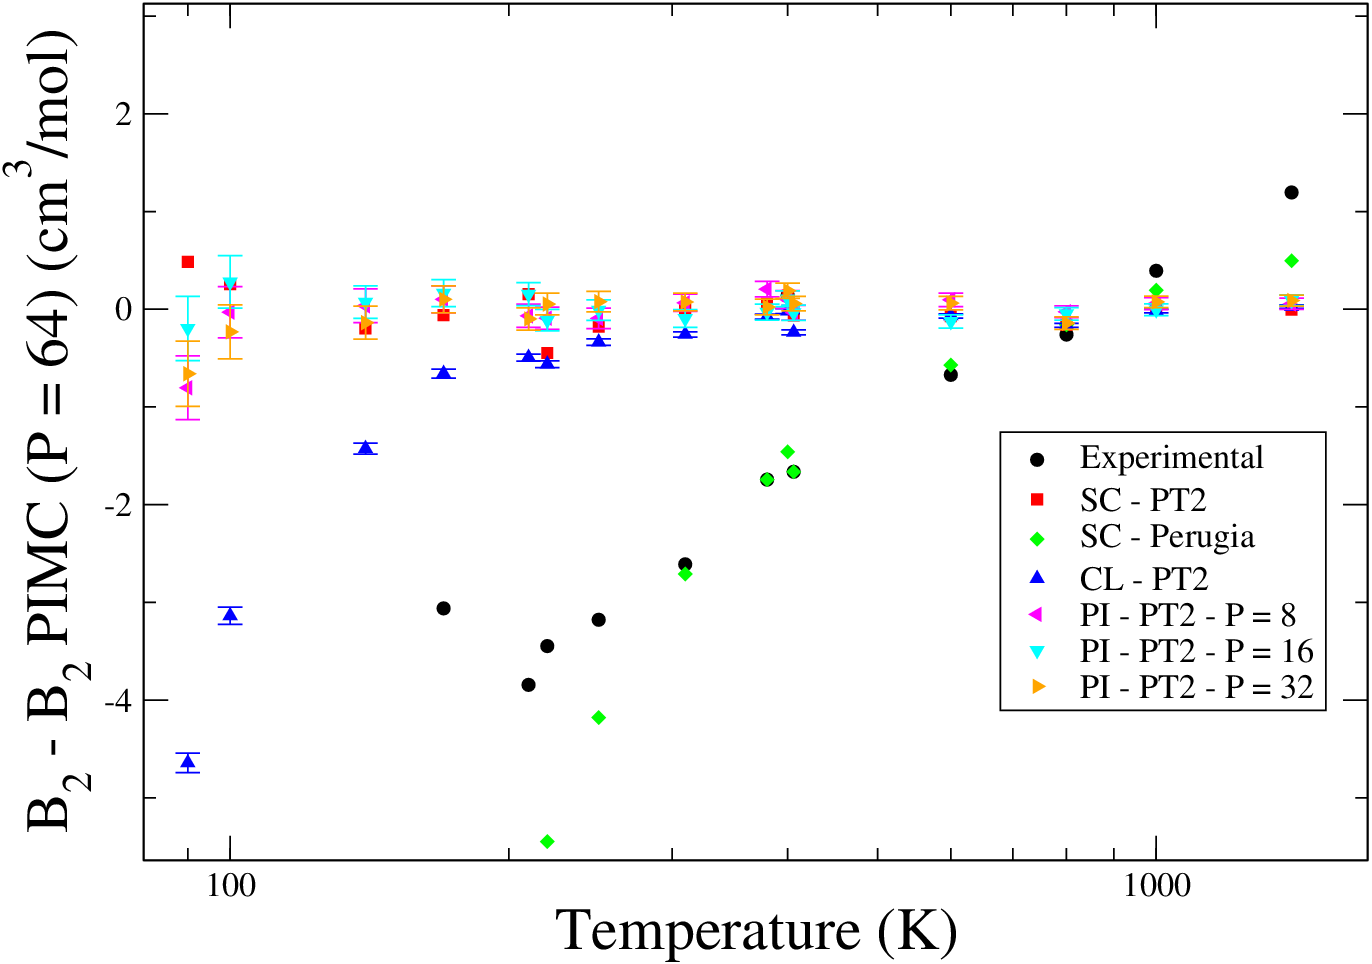
\includegraphics[scale=0.20,keepaspectratio]{Chapter-6/Figures/B2O2AllDiffPT2.png}
        \caption{Difference between various second virial coefficient ($B_2$) values compared against our most accurate PIMC results ($P$ = 64). Experimental results are from Refs. \cite{Bartolomei2010,Dymond}; SC - PT2 and SC - Perugia are from semi-classical results of Bartolomei et al. \cite{Bartolomei2010} by using the PT2 and Perugia \PESs{} \cite{Aquilanti1999} respectively; CL - PT2 and PI - PT2 are our classical and PIMC results respectively using the PT2 \PESs{}.}
        \label{fig:B2O2AllDiffPT2}
    \end{figure}

    From Fig. \ref{fig:B2O2AllDiffPT2}, we observe a trend very similar to that of Fig. \ref{fig:B2O2AllDiffMRCI}. Here too, it can be seen that the semi-classical PT2 calculations performed by Bartolomei et al. \cite{Bartolomei2010} agrees with our PIMC calculations for the same \PESs{}, better than other semi-classical or classical calculations. Our PIMC calculations have converged for all temperatures investigated. Also, the experimental and the SC-Perugia values deviate the largest. For SC-Perugia calculations, this can be explained by the fact that their values are outdated and also because the use of different \PESs{} than ours. Finally, we can see that our classical values start to deviate significantly from the PIMC results for temperatures $T \le 300K$.

    \section{Conclusions}
        We have calculated fully quantum second virial coefficients for the oxygen dimer based on recent \abinitio{} \\PESs{} due to Bartolomei et al. \cite{Bartolomei2010}. We have implemented our orientation sampling algorithm in PIMC calculations. We observed good agreement with most accurate semi-classical values available in literature. These results add further confidence on the capabilities of the algorithm in combination with PIMC to predict accurate quantum virial coefficients.

\chapter{Water}
\label{chap:h2o}
\section{Recent developments}
    \label{sec:introduction}
        Water in its various phases has been the subject of a large number of theoretical, experimental and computational studies owing to its ubiquitous presence in nature. A number of these studies have been attempted to predict the structure and possibly gain insight or provide explanations for the anomalies in its behavior. These anomalies include \cite{Szalewicz2009} the temperature of maximum density at 4$^\circ$ C, temperature dependent isothermal compressibility, high boiling temperature and large number of phases of ice. Although these are generally attributed to hydrogen bonding capabilities of the molecule, they are still a source of motivation for scientific studies that hope to uncover further insight. On a much similar note, the nature of interactions of water molecules have also been the primary goal of many studies because these help predict other thermodynamic, structural and several other properties of water at different conditions. Although highly accurate empirical potential models have been developed to study water, these often involve lumping of several interactions like quantum effects, many body interactions etc. Therefore an \abinitio{} treatment of the water molecules is often the preferred route owing to its superior accuracy.
        One of the first \abinitio{} treatments of water included the one by Kuharski and coworkers \cite{Kuharski1984,Kuharski1985}. The authors used Path Integral Monte Carlo (PIMC) method with rigid rotors to include nuclear quantum effects and analyze its effect on the radial distribution function with application to predicting structure properties. The first set of \abinitio{} PESs \cite{Popkie1973,Matsuoka1976,Niesar1989,Niesar1990,Corongiu1992,Millot1992,Millot1998} involved relatively small numbers of grid points in their studies. The development of the SAPT-ss and SAPT-pp potentials by Mas et al. \cite{Mas1997} involved over a thousand configurations of the dimer and the use of a 83-function basis set, and the resulting spectra and other properties were found to be in excellent agreement with experimental results at that time. The SAPT-pp potential involved a highly anisotropic function that was computationally expensive to evaluate. This motivated the development of the SAPT-5s potential which involved 5 unique symmetry sites and a more efficient form of the function. Bukowski and coworkers \cite{Bukowski2007,Bukowski2008a,Bukowski2008b} performed calculations at the CCSD(T) level of theory using the same basis sets of SAPT-5s and reported the CCpol potential. Although it had a form similar to SAPT-5s, the CCpol potential had a polarization term that represented the bulk of the induction energy. They also observed excellent agreement of the their prediction over a wide range of properties. Cencek et al. \cite{Cencek2008} reported the CCpol-8s potential after applying a refitting procedure to the CCpol potential to obtain improved RMSE for the \abinitio{} energies. This set the benchmark for all \abinitio{} PESs by having the best agreement with experimental results. They added 3 more symmetry sites per molecule than the CCpol potential in order to improve their previous fits. Although the addition of 3 extra sites would have resulted in an increase in the computational cost, owing to the simple nature of the potential function involved, the adverse effects of adding more sites were somewhat nullified. More recently, G\'{o}ra et al. \cite{Gora2014} reported rigid two body and three-body potentials using the aug-CC-TZ quality basis set and observed better agreement to flexible benchmarks than even some of the flexible potentials. Since their two body fit involved a new polarization model which was more elaborate, they were able to achieve better results than all the previous PESs. Note that all potentials mentioned above involved the use of rigid monomers. Due to the severe complexity and the associated need for computational resources, not nearly as many flexible \abinitio{} potentials  exist as do rigid potentials. See e.g. \cite{Szalewicz2009} for a comprehensive review of PESs for the water molecule. Most recently, Jankowski et al.\cite{Jankowski2015} investigated several hybrid PESs that combined an existing rigid potential and a flexible potential, developed using the same ground-state geometries \cite{Leforestier2002}. The flexible correction involved in the hybrid PES is computed as the difference between the vibrationally averaged flexible potential and the same potential evaluated at its ground state geometry.

    \section{Methods}
    \label{sec:methods}
        \subsection{Hybrid PES}
        \label{subsec:hybridPES}
            Hybrid PESs are extremely useful because they allow us to compute second virial coefficients including monomer flexibility effects and are defined as the sum of a rigid potential and a flexible correction, which in turn is defined as the difference between the flexible potential computed using the flexible monomer geometries (denoted as $\mbf{r}_i$ for monomer $i$) and ground state geometries (denoted as $<\mbf{r}_i>_0$ for monomer $i$). The \emph{ad hoc} \abinitio{} PES we have employed is denoted as $V_{\text{CCpol-8sf*}}$ and is defined very similarly to CCpol-8sf \cite{Leforestier2012,Jankowski2015}. We provide the following expressions to exemplify the difference between the two: 
            \begin{subequations}
                \label{eq:hybridPESs}
                \begin{align}
                    V_{\text{CCpol-8sf*}} (R, \bm{\omega}_A, \bm{\omega}_B, \mbf{r}_A, \mbf{r}_B) &= V_{\text{CCpol2-QFH}} (R, \bm{\omega}_A, \bm{\omega}_B)\nonumber\\
                    &+ \big[ V_{\text{SAPT-5s'fIR}} (R, \bm{\omega}_A, \bm{\omega}_B, <\mbf{r}_A>_T, <\mbf{r}_B>_T)\nonumber\\
                    &- V_{\text{SAPT-5s'fIR}} (R, \bm{\omega}_A, \bm{\omega}_B, <\mbf{r}_A>_0, <\mbf{r}_B>_0) \big]\label{eq:ccpol8sf*}\\
                    V_{\text{CCpol-8sf}} (R, \bm{\omega}_A, \bm{\omega}_B, \mbf{r}_A, \mbf{r}_B) &= V_{\text{CCpol-8s}} (R, \bm{\omega}_A, \bm{\omega}_B)\nonumber\\
                    &+ \big[ V_{\text{SAPT-5s'fIR}} (R, \bm{\omega}_A, \bm{\omega}_B, \mbf{r}_A, \mbf{r}_B)\nonumber\\
                    &- V_{\text{SAPT-5s'fIR}} (R, \bm{\omega}_A, \bm{\omega}_B, <\mbf{r}_A>_0, <\mbf{r}_B>_0) \big]\label{eq:ccpol8sf}
                \end{align}
            \end{subequations}
            where $R$ represents the intermolecular distance; $\bm{\omega}_i$ denotes the orientation vectors of molecule $i$; $\mbf{r}_i \equiv (r_{i,1}, r_{i,2}, \theta_i)$ denotes the geometry of molecule $i$ given in terms of two bond lengths and one bond angle; $<\mbf{r}_i>_T$ and $<\mbf{r}_i>_0$ denotes the vibrationally averaged temperature-dependent and ground-state geometries respectively, of molecule $i$. The potential denoted as $V_{\text{SAPT-5s'fIR}}$ was reported by Szalewicz et al. \cite{Szalewicz2006} allowing monomer flexibility and the potential denoted as $V_{\text{CCpol2-QFH}}$ is the quadratic Feynman-Hibbs version of the rigid potential due to G\'{o}ra et al. \cite{Gora2014} and was used by Schultz et al. \cite{Schultz2015}.


            
            In order to be consistent, we have used the same vibrationally averaged ground-state geometry as that of CCpol2 (reported in Ref. \cite{Gora2014}) throughout our expression for CCpol-8sf*. Note that this ensures that we obtain the CCpol2-QFH potential if we use the ground-state geometry and evaluate CCpol-8sf*. As explained in Sec. \ref{sec:introduction}, we have chosen CCpol2 as the rigid potential in the definition CCpol-8sf* because of its superior quality as compared to CCpol-8s.
        
        \subsection{Virial coefficients}
            In this section, we briefly outline the procedure employed by Jankowski et al. \cite{Jankowski2015} to compute virial coefficients including monomer flexibility and quantum effects. Since our hybrid PES was slightly different from theirs (see Eq. \eqref{eq:hybridPESs}), a brief explanation of their procedure will help appreciate the differences in our calculations as a result.

            As a first step, they provide expressions for the classical second virial coefficient using a potential that has been averaged over intramonomer coordinates as:
            \begin{equation}
                \label{eq:B2cl}
                B_{\text{cl}} (T) = -\displaystyle\frac{1}{2} \int <f(T)>_{\omega_A, \omega_B} d\mbf{R}
            \end{equation}
            where the Mayer function $f(T)$ is given as:
            \begin{equation}
                \label{eq:fV0}
                f(T) = \exp ( -\beta <V>_0 (R, \mbf{\omega}_A, \mbf{\omega}_B) - 1)
            \end{equation}
            where $\beta = 1/k_\text{B} T$ and $<V>_0$ denotes the vibrationally average potential.

            The monomer flexibility contribution to the virial coefficient is computed using Eqs. \eqref{eq:B2cl}  and \eqref{eq:fV0} as:
            \begin{equation}
                \label{eq:deltaBFlex}
                \Delta B_\text{flex}^{<V>_0} = B_\text{cl}^{<V>_0} -  B_\text{cl}^{V(<r>_0)}
            \end{equation}
            
            Note that in our approach we do not involve the use of the vibrationally averaged potential $<V>_0$, rather we simply use the CCpol-8sf* potential in its stead. 

            To include quantum effects, a Takahashi Imada (TI) \cite{Takahashi1984} effective potential is defined as follows \cite{Schenter2002,Jankowski2015}:
            \begin{equation}
            \label{eq:chap7-TI}
                V^\text{TI}_\text{eff} = V_{\text{rigid}} + \displaystyle\frac{\hbar^2}{24 (k_\text{B} T)^2} \sum_{i = 1}^2 \left[ \frac{\mbf{F}_i^2}{M} + \sum_\alpha \frac{\tau_{\alpha i}^2}{I_\alpha} \right]
            \end{equation}
            where $\mbf{F}_i$ is the force exerted on molecule $i$ and $\tau_{\alpha i}, \alpha = 1, 2, 3,$ are the components of torque on the molecule $i$ along the principal axis $\alpha$ of the molecule (Note: $\mbf{F}_i$ and $\tau_{\alpha i}$ are computed using $V_{\text{rigid}}$). $M$ and $I_\alpha$ denote the mass and the principal moments of inertia of the molecule respectively.

            The quantum contribution to the virial coefficient denoted as $B_\text{QM}^\text{TI} (T)$ then is computed using $V^\text{TI}_\text{eff}$ (Eq. \eqref{eq:chap7-TI}) in place of $<V>_0$ in Eq. \eqref{eq:fV0} and evaluating the resulting Eq. \eqref{eq:B2cl}.

            The total virial coefficient is then computed simply as the sum of the two contributions, i.e.,
            \begin{equation}
                 B_\text{flex} (T) = B_\text{QM}^\text{TI} (T) + \Delta B_\text{flex}^{<V>_0}
            \end{equation}

            Note that in our approach, we use QFH effective potential instead to the TI version mentioned above. The expression for $V^\text{QFH}_\text{eff}$ used by Schultz et al. \cite{Schultz2015,Feynman}:
            \begin{equation}
                \label{eq:chap7-QFH}
                V^\text{QFH}_\text{eff} = V_{\text{rigid}} + \displaystyle\frac{\hbar^2}{12 k_\text{B} T} \sum_{i = 1}^2 \left[ \frac{1}{M} \nabla^2_{r_i} V_\text{rigid} + \frac{1}{2} \sum_k \frac{1}{I_{k,i}} \frac{\partial^2 V_\text{rigid}}{\partial \omega_{k,i}^2} \right]
            \end{equation}
            where $k$ is the sum over orientations $\omega_{k,i}$ defined for molecule $i$ in the principle axes of its moment of inertia.
            
            To summarize, we provide expressions for the second virial coefficient to exemplify the difference between the two calculations:
            \begin{subequations}
                \label{eq:B2Total}
                \begin{align}
                    B_\text{flex} (T) &= B_\text{QM}^\text{QFH} (T) + \Delta B_\text{flex}^{V_\text{CCpol-8sf*}}\label{eq:b2ccpol8sf*}\\
                    B_\text{flex} (T) &= B_\text{QM}^\text{TI} (T) + \Delta B_\text{flex}^{<V_\text{CCpol-8sf}>_0}
                \end{align}
            \end{subequations}
\section{Computational details}
    \label{sec:computational details}
        In order to compute precise values for virial coefficients and save computational costs, we compute differences of the virial coefficients from already computed values. Within the MSMC framework, this is simply achieved by defining the target configurational integral as \cite{Shaul2012}:
        \begin{equation}
            \Gamma (T) = \Gamma_{\text{CCpol-8sf*}} - \Gamma_{\text{CCpol2-QFH}}
        \end{equation}

        Note that CCpol-8sf* (Eq. \eqref{eq:ccpol8sf*}) is a sum of CCpol2-QFH and a flexible correction that is expected to be small. Thus $\Gamma (T)$ is also expected to be small over the entire region of configuration space and hence improve the precision of the calculation. Note that this is particularly true only for high temperatures and low order of virial coefficients. Generally, $\Gamma (T)$ tends to become large for lower temperatures and higher order of virial coefficients. Even when it is large, we expect to save on computational costs by using such a definition because we already have results for the CCpol2-QFH case as reported by Schultz et al. \cite{Schultz2015}. Note that the values and uncertainties reported by Schultz et al. have been interpolated for the temperatures investigated in this work using polynomial fits. We have used the same MSMC parameters as was done by Schultz et al. and hence, we chose not to repeat them here. This process was used for both second and third virial coefficient calculations. Note that we have used the non-additive three body potential of G\'{o}ra et al. \cite{Gora2014} in our third virial coefficient calculations.

        For computing the flexible potential SAPT-5s'fIR, we have obtained the vibrationally averaged temperature-dependent monomer geometries of Czak\'{o} et al. \cite{Czako2009}. Spline fits were used to evaluate geometries at the temperatures considered here. In order to avoid nonphysical values of the dimer energies, we have used an artificial spherical hard core of diameter $d = 1.2$\AA (i.e., the energy value for the CCpol-8sf* function was set to positive infinity if the intermolecular distance was less than $d$). For details regarding a similar procedure for the CCpol2-QFH case and other details pertaining to the use of the CCpol2-QFH PES that are not mentioned here, we point the reader to Ref. \cite{Schultz2015}. 

        We collected $10^8$ and $10^7$ configuration samples for the semi-classical second and third virial coefficients respectively, each including MC trials for translation and rotation with equal probability. Additionally, a coarse orientational average as explained by Benjamin et al. \cite{Benjamin2009} was applied by the inclusion of a MC trial for flipping (i.e., inversion of the molecules about their geometric centers). The minimum intermolecular distance at which this MC trial became active in the simulation was set to 20\AA and 10\AA for the second and third virial coefficient calculations respectively.

        Note: All simulations in this work were performed using MSMC and Etomica \cite{Schultz2015Etomica} package to compute virial coefficients.
\section{Results and discussion}
    \label{sec:results}
        In Fig. \ref{fig:B2SC-comparison}, we plot the difference between various models and the experimental results based correlation due to Harvey and Lemmon \cite{Harvey2004}. As can be seen, the results of Jankowski et al. \cite{Jankowski2015} calculated using the TI effective potential and including monomer flexibility effects seems to be in best agreement with the experimental results. Somewhat unexpectedly, the rigid calculations of Schultz et al. \cite{Schultz2015} seem to be agreeing better as compared to the present calculations including monomer flexibility by using temperature-dependent geometries of Czak\'{o} et al. The reason for this is not yet clear although we do have our concerns regarding certain assumptions made with respect to the definition of CCpol-8sf*.
        \begin{figure}[!htbp]
            \centering
            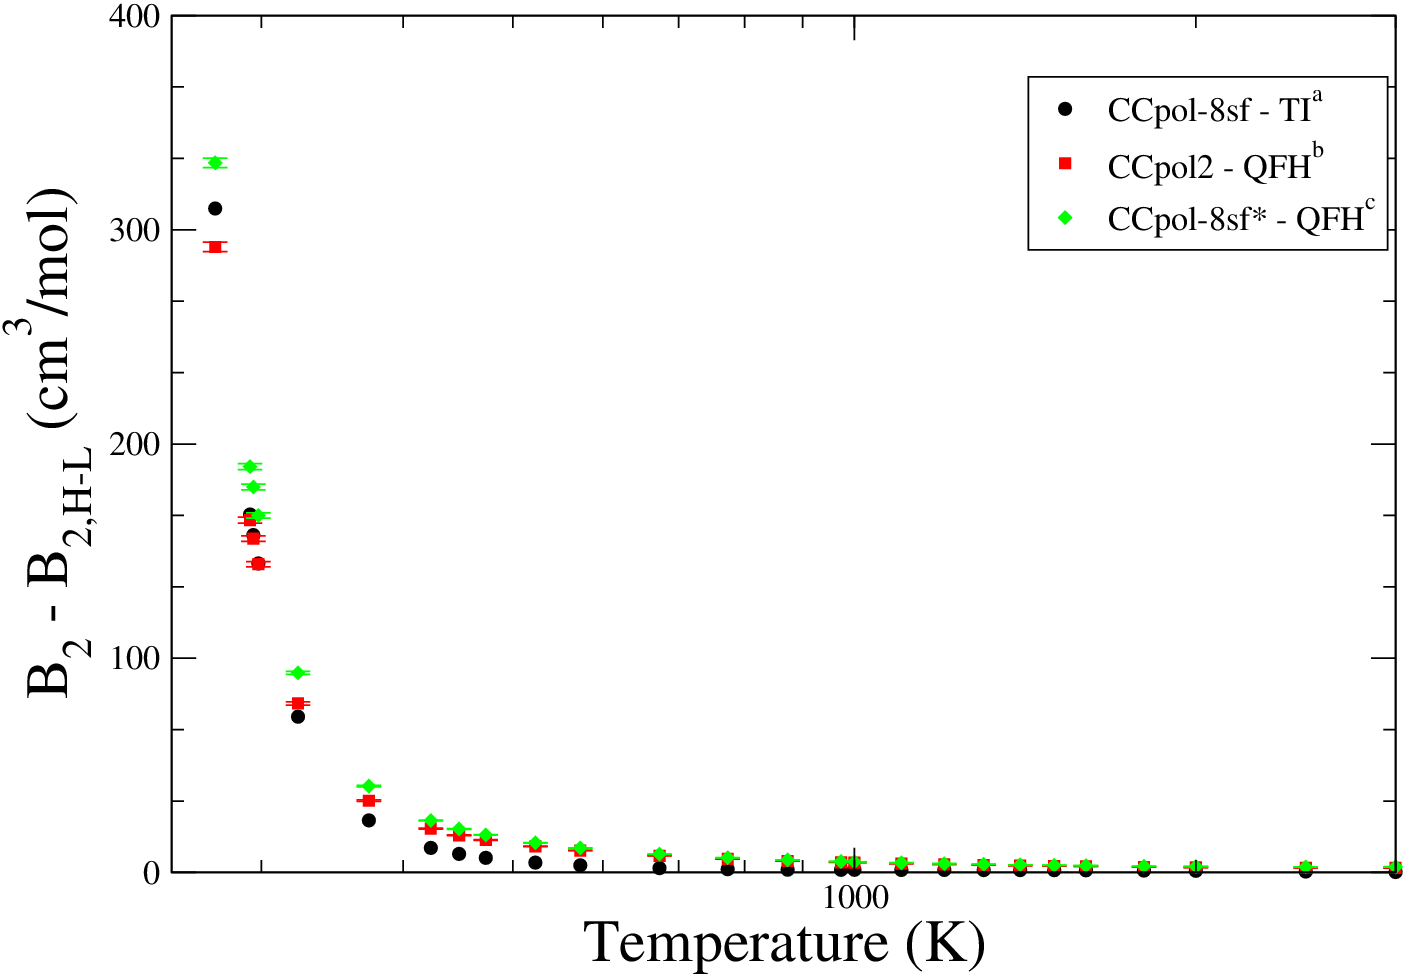
\includegraphics[width=10cm,keepaspectratio]{Chapter-7/Figures/B2SCAll.png}
            \caption{Comparison of the semi-classical second virial coefficient of water for various models including quantum effects, with the experiment based Harvey - Lemmon correlation \cite{Harvey2004} denoted as $B_{2,\text{H-L}}$. $^\text{a}$ - Results from Jankowski et al. \cite{Jankowski2015} using CCpol8sf TI effective potential and vibrational averaging; $^\text{b}$ - Results from Schultz et al. \cite{Schultz2015} using CCpol2 QFH effective potential; $^\text{c}$ - Results from this work using CCpol2 QFH effective potential and vibrationally averaged temperature-dependent geometries. Error bars where shown represent one standard deviation of the mean (68\% confidence interval).}
            \label{fig:B2SC-comparison}
        \end{figure}

        The primary concern of ours lies in the definition of the CCpol-8sf* potential (Eq. \eqref{eq:ccpol8sf*}). The argument made by Jankowski et al. \cite{Jankowski2015} that the definition of hybrid surfaces is made possible only if two (viz., the rigid and the flexible) potentials have been derived using the same ground-state monomer geometries, which is not the case in our calculations. Also, we have ignored embedding of the monomer in the dimer as performed for the flexible potential SAPT-5s'fIR by Jankowski et al. \cite{Jankowski2015}. We assumed that since we are using the ground-state geometries of the rigid potential within the flexible potential, this embedding need not be done. However, this could be significantly affecting the way in which the flexible potential is evaluated.

    \section{Conclusion}
    \label{chap7-sec:conclusion}
        Conclusion here.
    \section{Tabulated Results}
    \label{sec:chap7-tables}
        We report tabulated results for the virial coefficients of water in this section.
        \pgfplotstableset{
            begin table=\begin{longtable},
            end table=\end{longtable},
        }
        \pgfplotstabletypeset[
            columns/temperature/.style={
                string type,
                column name={Temperature(\si{\kelvin})}
            },
            columns/b2sc/.style={
                string type,
                column name=B$_2$(\si{cm^3/mol})
            },
            columns/b3sca/.style={
                string type,
                column name=B$^\text{A}_3$(\si{cm^6/mol^2})
            },
            columns/b3scna/.style={
                string type,
                column name=B$^\text{NA}_3$(\si{cm^6/mol^2})
            },
            columns/b3sctot/.style={
                string type,
                column name=B$^\text{Tot}_3$(\si{cm^6/mol^2})
            },
            every head row/.append style={before row={\caption{Second and third virial coefficients of nitrogen using the hybrid PES defined in Eq. \eqref{eq:ccpol8sf*} and evaluated based on Eq. \eqref{eq:b2ccpol8sf*}. B$^\text{A}_3$ and B$^\text{NA}_3$ represent the additive and non-additive contributions respectively, to the third virial coefficient. B$^\text{Tot}_3$ represents the full third virial coefficient value obtained by summing the additive and non-additive contributions. Values in parantheses are standard uncertainties in the rightmost digit(s).}\label{tab:h2oSCResults}\\\toprule},after row=\midrule\endfirsthead},
            every first row/.append style={before row={\multicolumn{5}{c}{\tablename\ \thetable{} -- Continued from previous page.}\\\toprule},after row=\midrule\endhead},
            every last row/.style={after row=\bottomrule},
        ]{Chapter-7/Tables/SCResultsTable.dat}


\chapter{Conclusions and Suggestions for Future Work}

%\chapter{Misc. 1}

%\chapter{Misc. 2}

%%%%%%%%%%%%%%%%%%%%%%%%%%%%%%%%%%%%%%%%%%%%%%%%%%%%%%%%%%%%%%%
% Appendices
%
% Because of a quirk in LaTeX (see p. 48 of The LaTeX
% Companion, 2e), you cannot use \include along with
% \addtocontents if you want things to appear the proper
% sequence. Since the PSU Grad School requires
%%%%%%%%%%%%%%%%%%%%%%%%%%%%%%%%%%%%%%%%%%%%%%%%%%%%%%%%%%%%%%%
\appendix
\Appendix{Orientation Move: Mathematical details}
\label{Appendix A}
    \section{Distances and Angles}
        In this section, we derive the mathematical formula for the most general case where the bond length is different for image 0, 1 and 2.
        \begin{figure}[!htbp]
            \centering
            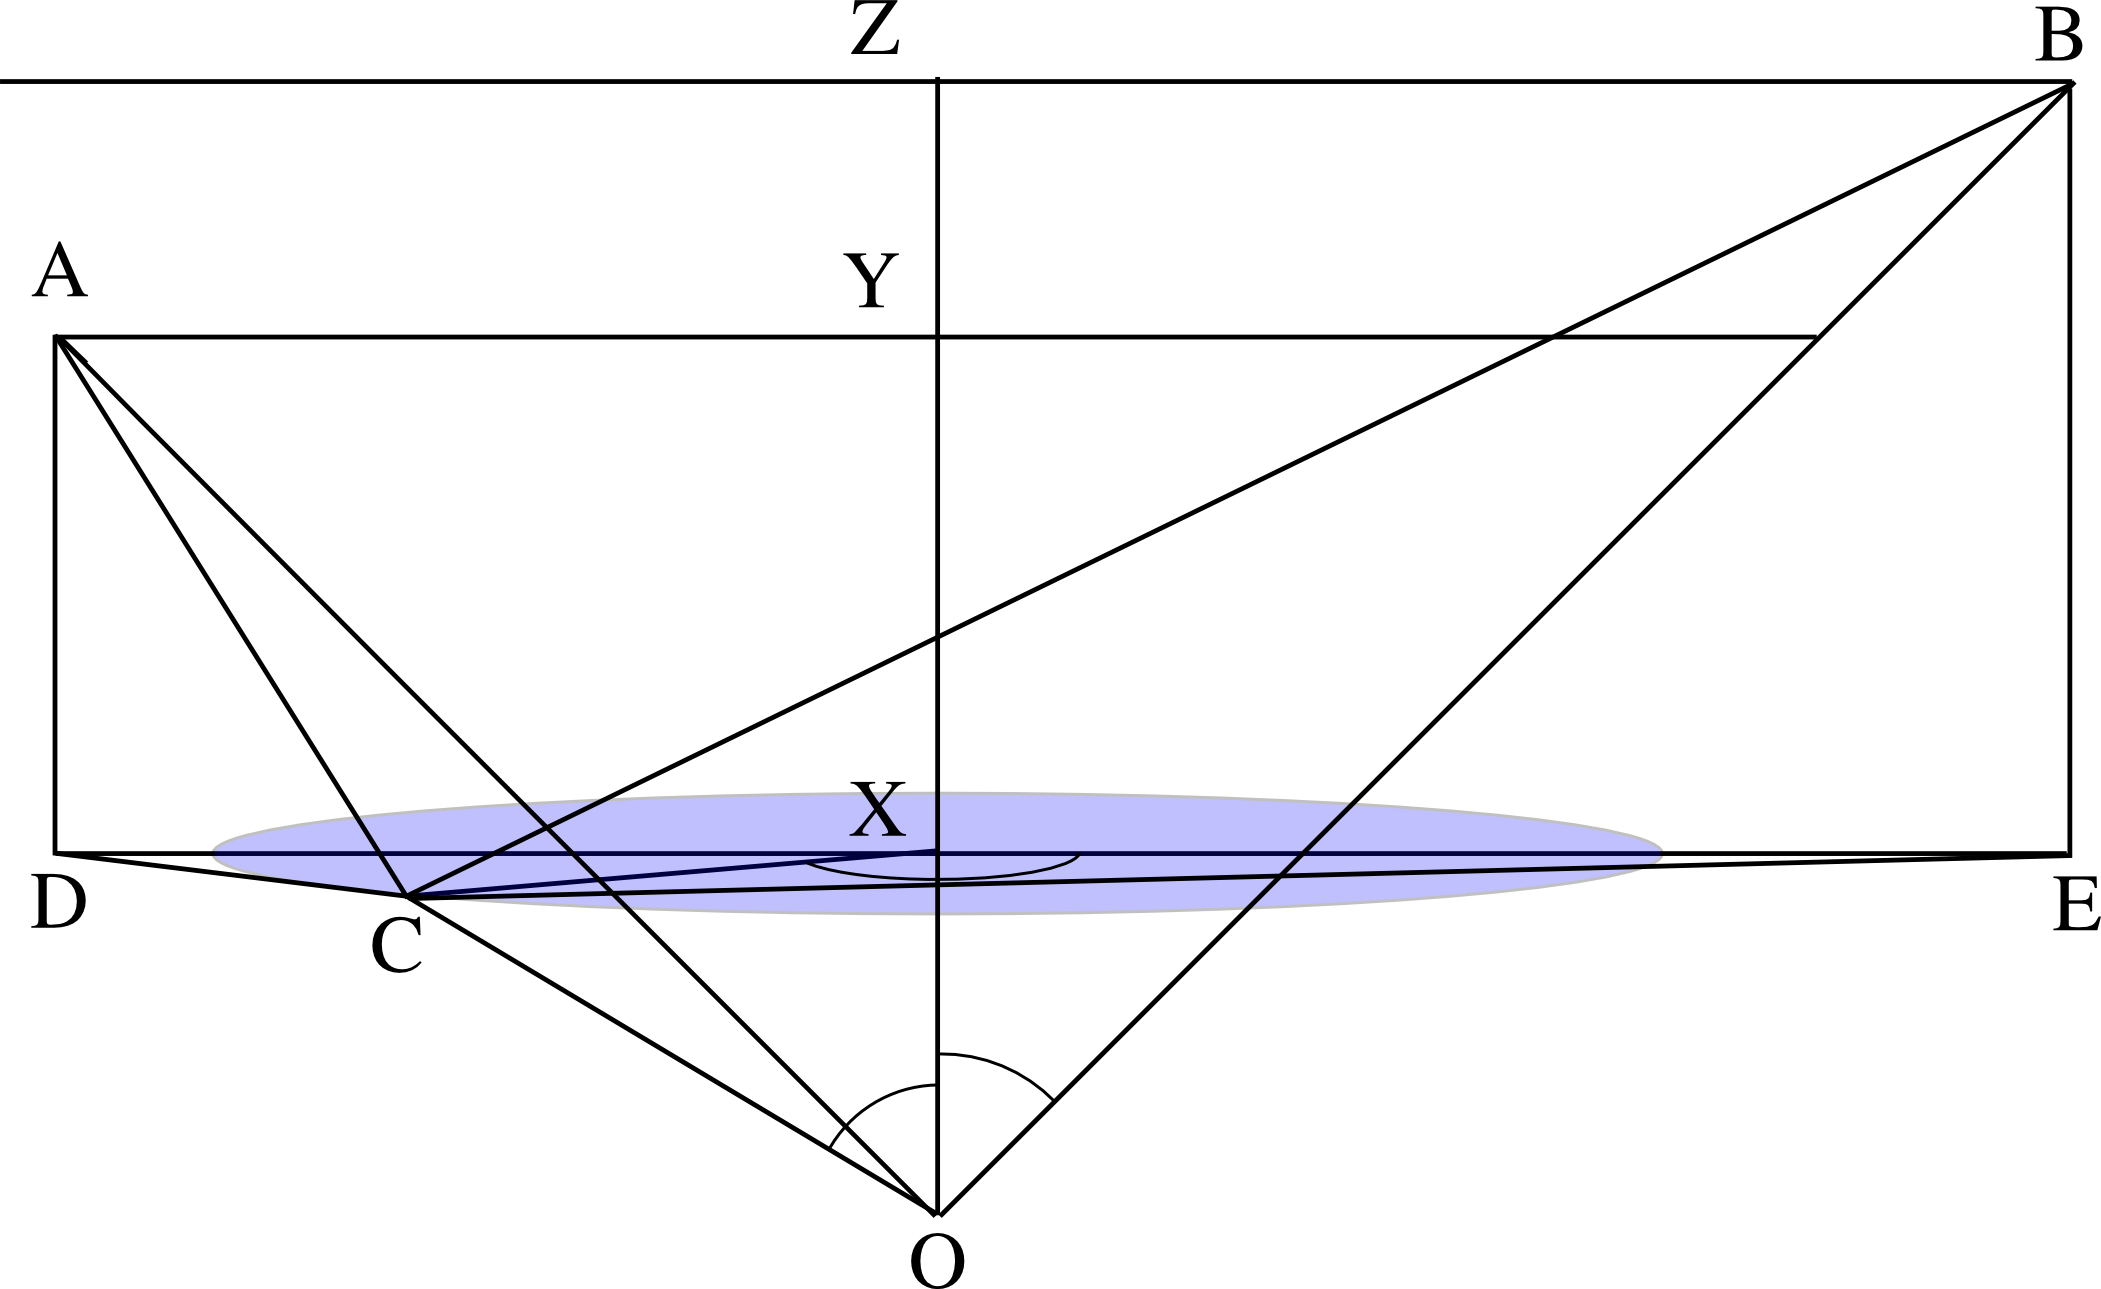
\includegraphics[scale=1.5,keepaspectratio]{Appendix-A/Figures/differentBondlength.png}
            \caption{Simple visualization of the distances involved}
            \label{fig:dist}
        \end{figure}
        Consider the locations of image 0, image 1 and image 2 at A, C and B respectively (see fig. \ref{fig:dist}). All beads and harmonic springs have been omitted from the figure for the sake of clarity. We define the following angles and distances to begin with:
        \begin{itemize}
            \item $\angle AOB = \psi$
            \item $\angle AOX = \angle XOB = \displaystyle\frac{\psi}{2}$
            \item $\angle COX = \alpha$
            \item $\angle CXE = \beta$
            \item $r_0 \equiv d_{OA} = \displaystyle\frac{b_0}{2} , \qquad r_1 \equiv d_{OC} = \frac{b_1}{2}, \qquad r_2 \equiv d_{OB} = \frac{b_2}{2}$
            \item The points O, X, Y and Z are collinear
        \end{itemize}

        In $\Delta AYO ,\angle AOY = \displaystyle\frac{\psi}{2}, \: \: \: \angle AYO = \frac{\pi}{2}$
        \begin{equation}
        \label{eq:ay}
            \Rightarrow d_{AY} = r_0  \sin \Big(\displaystyle\frac{\psi}{2}\Big), \: \: \: d_{OY} = r_0  \cos \Big(\displaystyle\frac{\psi}{2}\Big)
        \end{equation}

        In $\Delta BZO ,\angle BOZ = \displaystyle\frac{\psi}{2}, \: \: \: \angle BZO = \frac{\pi}{2}$
        \begin{equation}
        \label{eq:bz}
            \Rightarrow d_{BZ} = r_2  \sin \Big(\displaystyle\frac{\psi}{2}\Big), \: \: \: d_{OZ} = r_2  \cos \Big(\displaystyle\frac{\psi}{2}\Big)
        \end{equation}

        In $\Delta CXO ,\angle COX = \alpha, \: \: \: \angle CXO = \frac{\pi}{2}$
        \begin{equation}
        \label{eq:cx}
            \Rightarrow d_{XC} = r_1  \sin \big(\alpha\big), \: \: \: d_{OX} = r_1  \cos \big(\alpha\big)
        \end{equation}

        From the figure and eqns. \eqref{eq:ay}, \eqref{eq:bz} and \eqref{eq:cx}, we can clearly see the following:
        \begin{equation}
        \label{eq:adbe}
            \begin{aligned}
                d_{DX} &= d_{AY} = r_0  \sin \Big(\displaystyle\frac{\psi}{2}\Big)\\
                d_{EX} &= d_{BZ} = r_2  \sin \Big(\displaystyle\frac{\psi}{2}\Big)\\
                d_{XY} &= d_{AD} = d_{OY} - d_{OX} = r_0  \cos \Big(\displaystyle\frac{\psi}{2}\Big) - r_1  \cos \big(\alpha\big)\\
                d_{XZ} &= d_{BE} = d_{OZ} - d_{OX} = r_2  \cos \Big(\displaystyle\frac{\psi}{2}\Big) - r_1  \cos \big(\alpha\big)
            \end{aligned}
        \end{equation}

        In $\Delta DCX$, we have:
        \begin{equation}
        \label{eq:dc}
            \begin{aligned}
                \cos \big( \pi - \beta \big) &= \frac{d_{DX}^2 + d_{XC}^2 - d_{DC}^2}{2  d_{DX}  d_{XC}}\\
                \Rightarrow d_{DC}^2 &= d_{DX}^2 + d_{XC}^2 + 2  d_{DX}  d_{XC}  \cos \big( \beta \big)
            \end{aligned}
        \end{equation}

        In $\Delta ADC$, we have from eqs. \eqref{eq:adbe} and \eqref{eq:dc}:
        \begin{equation}
        \label{eq:ac}
            \begin{aligned}
                d_{AC}^2 &= d_{AD}^2 + d_{DC}^2\\
                &= \Bigg[ {\Big(r_0  \cos \Big(\displaystyle\frac{\psi}{2}\Big) - r_1  \cos \big(\alpha\big) \Big)}^2 + r_1^2  \sin^2 \big( \alpha \big)\\
                &+ r_0^2  \sin^2 \Big(\displaystyle\frac{\psi}{2}\Big) + 2  r_0  r_1 \sin \big( \alpha \big)  \sin \Big(\displaystyle\frac{\psi}{2}\Big)  \cos \big( \beta \big) \Bigg]\\
                &= \Bigg[ r_0^2 + r_1^2 - 2  r_0  r_1  \cos \big( \alpha \big)  \cos \Big(\displaystyle\frac{\psi}{2}\Big)\\
                &+ 2  r_0  r_1 \sin \big( \alpha \big)  \sin \Big(\displaystyle\frac{\psi}{2}\Big)  \cos \big( \beta \big) \Bigg]
            \end{aligned}
        \end{equation}

        In $\Delta CXE$, we have:
        \begin{equation}
        \label{eq:ce}
            \begin{aligned}
                \cos \big( \beta \big) &= \frac{d_{XC}^2 + d_{EX}^2 - d_{CE}^2}{2  d_{XC}  d_{EX}}\\
                \Rightarrow d_{CE}^2 &= d_{XC}^2 + d_{EX}^2 - 2  d_{XC}  d_{EX}  \cos \big( \beta \big)
            \end{aligned}
        \end{equation}

        In $\Delta BCE$, we have from eqs. \eqref{eq:adbe} and \eqref{eq:ce}:
        \begin{equation}
        \label{eq:bc}
            \begin{aligned}
                d_{BC}^2 &= d_{BE}^2 + d_{CE}^2\\
                &= \Bigg[ {\Big(r_2  \cos \Big(\displaystyle\frac{\psi}{2}\Big) - r_1  \cos \big(\alpha\big) \Big)}^2 + r_1^2  \sin^2 \big( \alpha \big)\\
                &+ r_2^2  \sin^2 \Big(\displaystyle\frac{\psi}{2}\Big) - 2  r_1  r_2 \sin \big( \alpha \big)  \sin \Big(\displaystyle\frac{\psi}{2}\Big)  \cos \big( \beta \big) \Bigg]\\
                &= \Bigg[ r_1^2 + r_2^2 - 2  r_1  r_2  \cos \big( \alpha \big)  \cos \Big(\displaystyle\frac{\psi}{2}\Big)\\
                &- 2  r_1  r_2 \sin \big( \alpha \big)  \sin \Big(\displaystyle\frac{\psi}{2}\Big)  \cos \big( \beta \big) \Bigg]
            \end{aligned}
        \end{equation}

        Therefore, for the most general case with different bond lengths, from eqs. \eqref{eq:ac} and \eqref{eq:bc}, we have:
        \begin{equation}
            \begin{aligned}
                d_{AC}^2 + d_{BC}^2 &= r_0^2 + 2  r_1^2 + r_2^2 - 2  r_1  \cos \big( \alpha \big)  \cos \Big(\displaystyle\frac{\psi}{2}\Big)  \big( r_0 + r_2 \big)\\
                &+ 2  r_1  \sin \big( \alpha \big)  \sin \Big(\displaystyle\frac{\psi}{2}\Big)  \cos \big( \beta \big)  \big( r_0 - r_2 \big)
            \end{aligned}
        \end{equation}

        For the simple case where $r_0 = r_1 = r_2 = \displaystyle\frac{b}{2}$, we have:
        \begin{equation}
        \label{eq:final}
            d_{AC}^2 + d_{BC}^2 = b^2  \Big[ 1 - \cos \big( \alpha \big)  \cos \Big(\displaystyle\frac{\psi}{2}\Big) \Big]
        \end{equation}
    \section{Normalization of the Probability Distribution}
    \label{Appendix C}
    The unnormalized probability of the angle $\alpha$, including the degeneracy (circumference of the shaded circle in fig. \ref{fig:simple}) and Eq. \eqref{eq:Uh} is then given by:
    \ifkhExplicitP
        \begin{equation}
            \label{eq:piTildeAlpha}
            \tilde \pi({\mathbf b}_j: {\mathbf a}, \alpha)  = \pi b \sin(\alpha) \exp[-4k_h(1 - \cos(\psi/2) \cos(\alpha))]
        \end{equation}
    \else
        \begin{equation}
        \label{eq:piTildeAlpha}
            \tilde \pi({\mathbf b}_j: {\mathbf a}, \alpha)  = \pi b \sin(\alpha) \exp[-4k_h~b^2 (1 - \cos(\psi/2) \cos(\alpha))]
        \end{equation}
    \fi

    Since we choose angle $\beta$ uniformly, from fig.\ref{fig:simple} we can see that for a given $\alpha$, the probability of choosing a random $\beta$ is given by $\tilde \pi({\mathbf b}_j: {\mathbf a}, \beta)  = 1/[\pi b \sin (\alpha)]$. The probability distribution centered around ${\mathbf a}$, for placing any image $j$ is given as:
    \ifkhExplicitP
        \begin{equation}
        \label{eq:piTildeAlphaBeta}
            \begin{aligned}
                \tilde \pi({\mathbf b}_j: {\mathbf a}, \alpha, \beta) &= \tilde \pi({\mathbf b}_j: {\mathbf a}, \alpha)  \tilde \pi({\mathbf b}_j: {\mathbf a}, \beta)\\
                &= \exp[-4k_h (1 - \cos(\psi/2) \cos(\alpha))]
            \end{aligned}
        \end{equation}
    \else
        \begin{equation}
        \label{eq:piTildeAlphaBeta}
            \begin{aligned}
                \tilde \pi({\mathbf b}_j: {\mathbf a}, \alpha, \beta) &= \tilde \pi({\mathbf b}_j: {\mathbf a}, \alpha)  \tilde \pi({\mathbf b}_j: {\mathbf a}, \beta)\\
                &= \exp[-4k_h~b^2 (1 - \cos(\psi/2) \cos(\alpha))]
            \end{aligned}
        \end{equation}
    \fi

    Since we are generating points on the surface of a sphere, the area element $dA$ we use for normalization of Eq.\eqref{eq:piTildeAlphaBeta}) is the same as the area element in spherical coordinates given as $dA = (b/2) \sin(\alpha) d\alpha \, d\beta$. Note that because the distribution is centered around $a$, $dA$ is written in terms of $\alpha$ and $\beta$ and not in terms of the actual spherical coordinates $\phi_n$ and $\theta$ of image $n$. For the special case of $\psi = \pi$ since the r.h.s. of Eq. \eqref{eq:Uh} becomes independent of $\alpha$, we can choose it just like $\beta$, i.e., at random, uniformly on $[0, 2\pi]$. Therefore the normalized probability $\tilde \pi({\mathbf b}_j: {\mathbf a}) $ of placing any image $j$ is given as:
    \begin{equation}
    \label{eq:piTildebj}
        \begin{aligned}
            \tilde \pi({\mathbf b}_j: {\mathbf a}) &= \frac{\tilde \pi({\mathbf b}_j: {\mathbf a}, \alpha, \beta) }{\displaystyle\int_{\alpha = 0}^\pi \int_{\beta = 0}^{2 \pi} \tilde \pi({\mathbf b}_j: {\mathbf a}, \alpha, \beta) dA}\\
            &=
            \begin{cases}
                \displaystyle\frac{\kappa \times \exp[\kappa \cos (\alpha)]}{\exp[\kappa] - \exp[-\kappa]} & \text{if} \qquad \psi \ne \pi\\
                \displaystyle\frac{1}{2 \pi b} & \text{if} \qquad \psi = \pi\\
            \end{cases}
        \end{aligned}
    \end{equation}
    \ifkhExplicitP
        where $\kappa = 4 \cos(\psi/2) k_h$
    \else
        where $\kappa = 4 \cos(\psi/2) k_h~b^2$
    \fi

    The cumulative distribution function $C(\alpha)$ can then be evaluated as:
    \begin{equation}
    \label{eq:cdf}
        \begin{aligned}
            C(\alpha) &= \frac{\displaystyle\int_{\alpha = 0}^\alpha \int_{\beta = 0}^{2 \pi} \tilde \pi({\mathbf b}_j: {\mathbf a}, \alpha, \beta) dA}{\displaystyle\int_{\alpha = 0}^\pi \int_{\beta = 0}^{2 \pi} \tilde \pi({\mathbf b}_j: {\mathbf a}, \alpha, \beta) dA}\\
            &= \displaystyle\frac{1 - \exp \big[\kappa [1 - \cos (\alpha)] \big]}{1 - \exp [-2 \kappa]}
        \end{aligned}
    \end{equation}

\Appendix{Bond Length Move: Mathematical Details}
\label{Appendix B}
    To sample the bond lengths directly (albeit approximately), we approximate $y$ (eq. \eqref{eq:y}) with a second-order Taylor series about its minimum $b_m$ (Eq. \eqref{eq:bm}), and diagonalize the Hessian to yield a set of normal mode coordinates and associated eigenvalues, which can each be sampled as independent Gaussians. The elements of the Hessian matrix $M$ are given by:
    \begin{equation}
        \begin{aligned}
            M_{ij} &= \begin{cases}
            - k_{h}  \cos (\hat \theta) & \text{if} \: \: \: | i - j | = 1\\
            0 & \text{if} \: \: \: | i - j | >= 2
            \end{cases}\\
            M_{ii} &= 2  k_{h} + \frac{2}{b_{m}^2} + \frac{\beta}{P}  {\frac{d^2 u}{d b_i^2} \Bigg|}_{b_i = b_{m}}\\
        \end{aligned}
    \end{equation}

    where $\hat \theta$ is the nominal value of $\theta_{ij}$ as given by eq. \eqref{eq:thetaHat}.

    \section{The uniform mode}
        The mode which contributes equally to towards all the bond lengths is called the uniform mode. The actual distribution of the its normal mode coordinate $\eta_u$ is not Gaussian and hence choosing from a Gaussian distribution would be wrong. For the case of the normal mode, choosing its coordinate and summing up its contribution towards each bond length is equivalent to choosing the average bond length of the system itself. So, we collect histograms of the average bond length of the system right from the start of the simulation. We choose the normal mode coordinate from a Gaussian distribution at random, until 1000 bond length change moves have been performed. At this point, we have collected a significant enough histogram from which to choose the average bond length value from. Also, we adjust the histogram every 100 moves after the first 1000 moves as explained below. For all other modes, we choose their normal mode coordinate from their respective Gaussian distributions.

    \subsection{Adjusting the histogram}
        We start at the center of the histogram by identifying the bin that has the highest probability value. Let $n_{vis}$ denote the number of times a bin has been visited and $p_{10}$ denote the probability of a bin `p' with $n_{vis} = 10$. Let the total number of bins that were adjusted be $n_{adj}$. We move right and left from the center and increase the probability of visiting a bin to a certain value based on the following:
        \begin{itemize}
            \item If $n_{vis}$ is $0$ , set $n_{vis} = 10, \: \: \: p = p_{10}$ and $n_{adj}++$
            \item If $0 < n_{vis} < 10$, set $n_{vis} = 10$ and $p = p_{10}$
            \item Repeat left and right until $n_{adj} = 20$
        \end{itemize}

        It should be noted that these values were arrived at after considering different possible options and their combinations.

    \subsection{Generating a configuration}
        Let $A (P \times P)$ and $\lambda (P \times 1)$ denote the matrix of eigenvectors  and eigenvalues of $M$ respectively. Let $\eta_i$ and $\sigma_i$ denote the normal mode coordinate and the width of the Gaussian distribution of the $i^{th}$ mode respectively. Let $r_i$ be a random number from the $i^{th}$ Gaussian distribution. Let $b^{new}_j$ denote the new bond length generated for the $j^{th}$ image. We have the following relationships:
        \begin{equation}
            \begin{aligned}
                \sigma_i &= \frac{1}{\sqrt \lambda_i}\\
                \eta_i &= r_i  \sigma_i\\
                b_j^{new} &= b_m + \displaystyle\sum\limits_{i=0}^P A_{ij}  \eta_i\\
                \text{where,} \: \: \: {\frac{\partial y}{\partial b_i} \Bigg|}_{b_i = b_m} &= 0
            \end{aligned}
        \end{equation}

        The probability $\tilde \pi({\mathbf b})$, of generating a configuration of $P$ new bond lengths based on the method described above is given by:-
        \begin{equation}
            \tilde \pi({\mathbf b}) = \exp \Bigg[ \displaystyle\sum\limits_{i=0}^{P-1} - \frac{1}{2}  r_i^2 \Bigg]
        \end{equation}

%%%%%%%%%%%%%%%%%%%%%%%%%%%%%%%%%%%%%%%%%%%%%%%%%%%%%%%%%%%%%%%
% ESM students need to include a Nontechnical Abstract as the %
% last appendix.                                              %
%%%%%%%%%%%%%%%%%%%%%%%%%%%%%%%%%%%%%%%%%%%%%%%%%%%%%%%%%%%%%%%
% This \include command should point to the file containing
% that abstract.
%\include{nontechnical-abstract}
%%%%%%%%%%%%%%%%%%%%%%%%%%%%%%%%%%%%%%%%%%%
} % End of the \allowdisplaybreak command %
%%%%%%%%%%%%%%%%%%%%%%%%%%%%%%%%%%%%%%%%%%%

%%%%%%%%%%%%%%%%
% BIBLIOGRAPHY %
%%%%%%%%%%%%%%%%
% You can use BibTeX or other bibliography facility for your
% bibliography. LaTeX's standard stuff is shown below. If you
% bibtex, then this section should look something like:

\bibliographystyle{fomms}
\addcontentsline{toc}{chapter}{Bibliography}
\bibliography{masterReferences}

%
%\begin{thebibliography}{99}
%\addcontentsline{toc}{chapter}{Bibliography}
%\frenchspacing

%\bibitem{Wisdom87} J. Wisdom, ``Rotational Dynamics of Irregularly Shaped Natural Satellites,'' \emph{The Astronomical Journal}, Vol.~94, No.~5, 1987  pp. 1350--1360.

%\bibitem{G&H83} J. Guckenheimer and P. Holmes, \emph{Nonlinear Oscillations, Dynamical Systems, and Bifurcations of Vector Fields}, Springer-Verlag, New York, 1983.

%\end{thebibliography}
%

%\backmatter

% Vita
%\vita{SupplementaryMaterial/Vita}

\end{document}

